% mycsrf cloak file
%
% (c) Karsten Reincke, Frankfurt a.M. 2010, 2011, ff.
%
% This file is licensed under the Creative Commons Attribution 3.0 Germany
% License (http://creativecommons.org/licenses/by/3.0/de/): 
% For details see teh file LICENSE in the top directory
%
% select the document class
% S.26: [ 10pt|11pt|12pt onecolumn|twocolumn oneside|twoside notitlepage|titlepage final|draft
%         leqno fleqn openbib a4paper|a5paper|b5paper|letterpaper|legalpaper|executivepaper openrigth ]
% S.25: { article|report|book|letter ... }
%
% oder koma-skript S.10 + 16
\documentclass[
  DIV=calc,
  BCOR=5mm,
  12pt,
  headings=small,
  twoside,
  abstract=true,
  toc=bib,
  english,ngerman]{scrartcl}
  
%%% (1) general configurations %%%
\usepackage[utf8]{inputenc}

%%% (2) language specific configurations %%%
\usepackage[]{a4,babel}
\selectlanguage{ngerman}

% package for improving the grey value and the line feed handling
\usepackage{microtype}

%language specific quoting signs
\usepackage{csquotes}

% jurabib configuration
\usepackage[see]{jurabib}
\bibliographystyle{jurabib}
% mycsrf German jurabib configuration include module file 
%
% (c) Karsten Reincke, Frankfurt a.M. 2012, ff.
%
% This file is licensed under the Creative Commons Attribution 3.0 Germany
% License (http://creativecommons.org/licenses/by/3.0/de/): 
% For details see teh file LICENSE in the top directory

% the first time cite with all data, later with shorttitle
\jurabibsetup{citefull=first}

%%% (1) author / editor list configuration
%\jurabibsetup{authorformat=and} % uses 'und' instead of 'u.'
% therefore define your own abbreviated conjunction: 
% an 'and before last author explicetly written conjunction

% for authors in citations
\renewcommand*{\jbbtasep}{\ u.\ } % bta = between two authors sep
\renewcommand*{\jbbfsasep}{,\ } % bfsa = between first and second author sep
\renewcommand*{\jbbstasep}{\ u.\ }% bsta = between second and third author sep
% for editors in citations
\renewcommand*{\jbbtesep}{\ u.\ } % bta = between two authors sep
\renewcommand*{\jbbfsesep}{,\ } % bfsa = between first and second author sep
\renewcommand*{\jbbstesep}{\ u.\ }% bsta = between second and third author sep

% for authors in literature list
\renewcommand*{\bibbtasep}{\ u.\ } % bta = between two authors sep
\renewcommand*{\bibbfsasep}{,\ } % bfsa = between first and second author sep
\renewcommand*{\bibbstasep}{\ u.\ }% bsta = between second and third author sep
% for editors  in literature list
\renewcommand*{\bibbtesep}{\ u.\ } % bte = between two editors sep
\renewcommand*{\bibbfsesep}{,\ } % bfse = between first and second editor sep
\renewcommand*{\bibbstesep}{\ u.\ }% bste = between second and third editor sep

% use: name, forname, forname lastname u. forname lastname
\jurabibsetup{authorformat=firstnotreversed}
\jurabibsetup{authorformat=italic}

%%% (2) title configuration
% in every case print the title, let it be seperated from the 
% author by a colon and use the slanted font
\jurabibsetup{titleformat={all,colonsep}}
%\renewcommand*{\jbtitlefont}{\textit}

%%% (3) seperators in bib data
% separate bibliographical hints and page hints by a comma
\jurabibsetup{commabeforerest}

%%% (4) specific configuration of bibdata in quotes / footnote
% use a.a.O if possible
\jurabibsetup{ibidem=strict}
% replace ugly a.a.O. by ders., a.a.O. resp. ders., ebda.
% but if there are more than one author or girl writers?
\AddTo\bibsgerman{
  \renewcommand*{\ibidemname}{Ds.,\ a.a.O.}
  \renewcommand*{\ibidemmidname}{ds.,\ a.a.O.}
}
\renewcommand*{\samepageibidemname}{Ds.,\ ebda.}
\renewcommand*{\samepageibidemmidname}{ds.,\ ebda.}

%%% (5) specific configuration of bibdata in bibliography
% ever an in: before journal and collection/book-titles 

\renewcommand*{\bibjtsep}{in:\ }
\renewcommand*{\bibbtsep}{in:\ }

% ever a colon after author names 
\renewcommand*{\bibansep}{:\ }
% ever a semi colon after the title 
\renewcommand*{\bibatsep}{;\ }
% ever a comma before date/year
\renewcommand*{\bibbdsep}{,\ }

% let jurabib insert the S. and p. information
% no S. necessary in bib-files and in cites/footcites
\jurabibsetup{pages=format}

% use a compressed literature-list using a small line indent
\jurabibsetup{bibformat=compress}
\setlength{\jbbibhang}{1em}

% which follows the design of the cites and offers comments
\jurabibsetup{biblikecite}

% print annotations into bibliography
\jurabibsetup{annote}
\renewcommand*{\jbannoteformat}[1]{{ \itshape #1 }}

%refine the prefix of url download
\AddTo\bibsgerman{\renewcommand*{\urldatecomment}{Referenzdownload: }}

% we want to have the year of articles in brackets
\renewcommand*{\bibaldelim}{(}
\renewcommand*{\bibardelim}{)}

%Umformatierung des Reihentitels und der Reihennummer
\DeclareRobustCommand{\numberandseries}[2]{%
\unskip\unskip%,
\space\bibsnfont{(=~#2}%
\ifthenelse{\equal{#1}{}}{)}{, [Bd./Nr.]~#1)}%
}%

%Umformatierung Referenzverweises
\usepackage{xpatch}
\AfterFile{dejbbib.ldf}{%
  \xapptocmd{\bibsgerman}{%
     \def\inname{\ifjboxford in:\else\ifjbchicago in:\else in:\fi\fi}%
    \def\incollinname{\ifjboxford in:\else\ifjbchicago in:\else in:\fi\fi}%
  }{}{}%
}

% the field printed before ISBN, ISSN or URL is the bibfield note
% Hence: If you insert into the field note the type of the literature
% [ Print | [FreeWeb | BibWeb] / [ PDF | HTML ] ] then you now
% get entries like:
% Print: ISBN ....
% BibWeb / PDF => http...
% That's nice for dealing with electronic sources correctly
\DeclareRobustCommand{\jbissn}[1]{\unskip:\space ISSN #1}%
\DeclareRobustCommand{\jbisbn}[1]{\unskip:\space ISBN #1}%

\DeclareRobustCommand{\biburlprefix}{$\Rightarrow$ }
\DeclareRobustCommand{\biburlsuffix}{}



% language specific hyphenation
%mycsrfk Hyphenation Include Module text
%
% (c) Karsten Reincke, Frankfurt a.M. 2012, ff.
%
% This file is licensed under the Creative Commons Attribution 3.0 Germany
% License (http://creativecommons.org/licenses/by/3.0/de/): 
% For details see teh file LICENSE in the top directory
%


\hyphenation{ Mehr-stimmig-keit Musik-wissen-schaft-ler}



%%% (3) layout page configuration %%%

% select the visible parts of a page
% S.31: { plain|empty|headings|myheadings }
%\pagestyle{myheadings}
\pagestyle{headings}

% select the wished style of page-numbering
% S.32: { arabic,roman,Roman,alph,Alph }
\pagenumbering{arabic}
\setcounter{page}{1}

% select the wished distances using the general setlength order:
% S.34 { baselineskip| parskip | parindent }
% - general no indent for paragraphs
\setlength{\parindent}{0pt}
\setlength{\parskip}{1.2ex plus 0.2ex minus 0.2ex}


%%% (4) general package activation %%%
%\usepackage{utopia}
%\usepackage{courier}
%\usepackage{avant}
\usepackage[dvips]{epsfig}

% graphic

\usepackage{array}
\usepackage{shadow}
\usepackage{fancybox}

\usepackage{tikz}
\usetikzlibrary{arrows}
\usetikzlibrary{shapes,snakes}
\usetikzlibrary{positioning}
\usetikzlibrary{decorations.text}
\usetikzlibrary{trees}

\usepackage{amsmath}
\usepackage{amsfonts}


\usepackage{chngcntr}


%- start(footnote-configuration)

\deffootnote[1.5em]{1.5em}{1.5em}{\textsuperscript{\thefootnotemark)\ }}

% if document class = book: count footnotes from start to end
% \counterwithout{footnote}{chapter}
%- end(footnote-configuration)

% package for macking tables with broken lines
\usepackage{multirow}

%for using label as nameref
\usepackage{nameref}

%integrate nomenclature
% mycsrf  Deutsch Nomenclation Declaration Include Module 
%
% (c) Karsten Reincke, Frankfurt a.M. 2012, ff.
%
% This file is licensed under the Creative Commons Attribution 3.0 Germany
% License (http://creativecommons.org/licenses/by/3.0/de/): 
% For details see teh file LICENSE in the top directory

\usepackage[intoc]{nomencl}
\let\abbr\nomenclature
% Deutsche Überschrift
%\renewcommand{\nomname}{Abbreviations}
\renewcommand{\nomname}{Abkürzungen}

\setlength{\nomlabelwidth}{.20\hsize}
\renewcommand{\nomlabel}[1]{#1 \dotfill}
% reduce the line distance
\setlength{\nomitemsep}{-\parsep}
\makenomenclature


% depth of contents
\setcounter{secnumdepth}{5}
\setcounter{tocdepth}{5}

% Hyperlinks
\usepackage[breaklinks=true]{hyperref}
\hypersetup{bookmarks=true,breaklinks=true,colorlinks=true,citecolor=blue,draft=false}
\newcommand{\lnka}[1]{\href{#1}{\texttt{#1}}}
\newcommand{\lnkb}[2]{\href{#1}{\texttt{#1} (RDL: #2)}}

\usepackage{amssymb}

\usepackage{wasysym}
\usepackage{harmony}
\usepackage{musicography}
\usepackage{abc}
\usepackage{musixtex}
\usepackage{graphicx,color}
\usepackage{tabulary}
\usepackage{ulem}
\usepackage{picins}


\usepackage{pgf}
\usepackage{tikz}
\usetikzlibrary{arrows,automata}

%\usepackage{bigfoot}
\usepackage{verbatimbox}

% Unfortunately musixtex still uses outdated commands for
% establishing its own \bar command. Hence for enabling
% the use of musixtex we must 'redefine' these outdated commands:
\makeatletter
\DeclareOldFontCommand{\rm}{\normalfont\rmfamily}{\mathrm}
\DeclareOldFontCommand{\sf}{\normalfont\sffamily}{\mathsf}
\DeclareOldFontCommand{\tt}{\normalfont\ttfamily}{\mathtt}
\DeclareOldFontCommand{\bf}{\normalfont\bfseries}{\mathbf}
\DeclareOldFontCommand{\it}{\normalfont\itshape}{\mathit}
\DeclareOldFontCommand{\sl}{\normalfont\slshape}{\@nomath\sl}
\DeclareOldFontCommand{\sc}{\normalfont\scshape}{\@nomath\sc}
\makeatother 

\newcommand{\cadlab}[2]{Candenza-#1-#2}

\newcommand{\cad}[2]{
  \begin{flushright}\scshape\label{\cadlab{#1}{#2}}Cadenza-#1: #2\end{flushright}
}
\newcommand{\pnotes}[1]{\notes}

\newcommand{\acc}[0]{\textit}
\newcommand{\ra}[0]{$\rightarrow$}




\begin{document}

%% use all entries of the bliography
\nocite{*}

%%-- start(titlepage)
\titlehead{\textit{mycsrf} und Musik}
\subject{Release 1.1
}
\title{Musikwissenschaft mit \LaTeX}
\subtitle{Wie man Musikbeispiele mit Open-Source-Tools 
in seine wissenschaftliche Texte integriert.\\
{\small Eine selbstreferentielle Anleitung}}
\author{Karsten Reincke% mycsrf License Include Module
%
% (c) Karsten Reincke, Frankfurt a.M. 2012, ff.
%
% This file is licensed under the Creative Commons Attribution 3.0 Germany
% License (http://creativecommons.org/licenses/by/3.0/de/): 
% For details see teh file LICENSE in the top directory
%

\footnote{\textbf{This file is distributed under the terms of license XYZ}
Here, you can insert your conditions for using your text. Good examples
for such licenses are offered under \texttt{https://creativecommons.org/}. 
Traditionally it also possible to say : \emph{All rights reserved}.
In accordance to the license \texttt{CC BY 3.0 DE}, under which mycrsf
is released, you must finally point to mycsrf:
\newline 
{ \tiny \itshape [Format derived from \texttt{mind your Scholar Research
Framework} \copyright K. Reincke CC BY 3.0 DE http://fodina.de/mycsrf)] }}

}

%thanks entry cannot be combined with license footnote
%\thanks{den Autoren von KOMA-Script und denen von Jurabib}

\maketitle
%%-- end(titlepage)

% mycsrf 'for beeing included' snippet template
%
% (c) Karsten Reincke, Frankfurt a.M. 2012, ff.
%
% This text is licensed under the Creative Commons Attribution 3.0 Germany
% License (http://creativecommons.org/licenses/by/3.0/de/): Feel free to share
% (to copy, distribute and transmit) or to remix (to adapt) it, if you respect
% how you must attribute the work in the manner specified by the author(s):
% \newline
% In an internet based reuse please link the reused parts to mycsrf.fodina.de
% and mention the original author Karsten Reincke in a suitable manner. In a
% paper-like reuse please insert a short hint to mycsrf.fodina.de and to the
% original author, Karsten Reincke, into your preface. For normal quotations
% please use the scientific standard to cite
%

\begin{abstract}
\noindent \itshape
Der folgende Text stellt vor, wie man \LaTeX-Texte mit Open-Source-Mitteln um
musikalische Beispiele anreichert. Dazu sichtet er Notensatzprogramme, Editoren,
Konverter und Tools, die Notentexte erzeugen, verändern und in den \LaTeX-Text
einbetten. Und er skizziert, wie man ganze 'Produktionsketten' aus
Frontendsystemen, Konvertern und Backendsystemen 'zusammenstöpselt'.
Zuletzt entsteht so eine 'Landkarte' verschiedener Wege.
\end{abstract}




% this is only inserted to eject fault messages in texlipse
%\bibliography{../bib/literature}


\footnotesize
\tableofcontents

\normalsize

% mycsrf 'for beeing included' snippet template
%
% (c) Karsten Reincke, Frankfurt a.M. 2012, ff.
%
% This text is licensed under the Creative Commons Attribution 3.0 Germany
% License (http://creativecommons.org/licenses/by/3.0/de/): Feel free to share
% (to copy, distribute and transmit) or to remix (to adapt) it, if you respect
% how you must attribute the work in the manner specified by the author(s):
% \newline
% In an internet based reuse please link the reused parts to mycsrf.fodina.de
% and mention the original author Karsten Reincke in a suitable manner. In a
% paper-like reuse please insert a short hint to mycsrf.fodina.de and to the
% original author, Karsten Reincke, into your preface. For normal quotations
% please use the scientific standard to cite
%


%% use all entries of the bibliography

\subsection{Anlass}

\begin{quote}\textit{Was man braucht und nicht findet, muss man selbst herstellen.}
\end{quote}

Der Impuls, dieses Tutorial zu schreiben, kam mit dem Beginn eines größeren
musikwissenschaftlichen Projektes. Wie bei Textarbeiten üblich bestand meine
erste Aufgabe darin, meine Arbeit zu organisieren. Unnötige Tipparbeit ist mir
zuwider. Lieber verbringe ich doppelt so viel Zeit damit, die Anlegenheit zu
automatisieren. Glücklicherweise waren mir \acc{\LaTeX}, \acc{Bib\TeX}\ und
\acc{JabRef} längst schon vertraut. Meinen optimalen Zitierstil für das
Schreiben geisteswissenschaftlicher Arbeiten hatte ich bereits
konfiguriert\footcite[vgl.][\nopage wp]{Reincke2018a} und
dokumentiert\footcite[vgl][2ff]{Reincke2018b}. Damit hätte es im Kern losgehen
können.

Allerdings war für mich noch völlig unklar, wie man den Notentexte und -- vor
allem -- musikalische Analysen in \LaTeX-Texte einbindet. Nur das Gefühl sagte:
so schwierig würde das nicht werden. Am besten wäre natürlich ein
No\-ta\-tions\-system, das mich den Notentext hätte erfassen und -- sozusagen auf
Knopfdruck -- in meinen Text integrieren lassen. Danach galt es zu suchen.

Leider schwiegen sich meine sehr guten, einschlägigen \LaTeX-Bücher dazu
aus\footcite[ vgl.][vi ff, insbesondere 905 u. 909: das umfangreiche Register
erwähnt weder Musik im allgemeinen noch LilyPond oder MusiX\TeX im
Besonderen]{Voss2012a}, selbst wenn sie auch Randbereiche
behandelten\footcite[vgl.][vii ff, insbesondere 1080 u.
1087: auch dieses umfangreiche Register erwähnt weder Musik im allgemeinen noch
LilyPond oder MusiX\TeX im Besonderen.]{MitGoo2005a}. Die entsprechende
Internetrecherche überrollte mich dagegen: so viele Notationssysteme und Tools,
aber kein systematischer Überblick.\footnote{Rühmlich die Ausnahme von
\cite[][\nopage wp]{Thoma2018a}. Allerdings ging sie nicht in die Tiefe, die ich
benötigte.}

Wollte ich meine große Arbeit nicht gefährden und Sackgassen vermeiden, musste
ich die Möglichkeiten zuerst grundsätzlich sichten. Andernfalls hätte ich nur
eine Variante willkürlich herausgegriffen und wäre Gefahr gelaufen, schließlich
-- nachdem ich Zeit und Arbeit investiert gehabt hätte -- doch 'aufs falsche
Pferd gesetzt' zu haben. Was ich brauchte war -- sozusagen -- eine technisch
fundierte 'Landkarte' der Methoden und Tools, die mir den besten Weg weisen
konnte. Und so traf mich -- wieder einmal -- die Erkenntnis:

\begin{quote}\textit{Programme und Tutorials, die man braucht, aber im Netz
nicht findet, muss man selbst schreiben und -- sofern man sich als Teil der
Open-Source-Community versteht -- als Ausgleich für die schon erhaltenen
freie Software wieder an die  Allgemeinheit 'zurück'geben.}
\end{quote}



% this is only inserted to eject fault messages in texlipse
%\bibliography{../bib/literature}


% mycsrf 'for beeing included' snippet template
%
% (c) Karsten Reincke, Frankfurt a.M. 2012, ff.
%
% This text is licensed under the Creative Commons Attribution 3.0 Germany
% License (http://creativecommons.org/licenses/by/3.0/de/): Feel free to share
% (to copy, distribute and transmit) or to remix (to adapt) it, if you respect
% how you must attribute the work in the manner specified by the author(s):
% \newline
% In an internet based reuse please link the reused parts to mycsrf.fodina.de
% and mention the original author Karsten Reincke in a suitable manner. In a
% paper-like reuse please insert a short hint to mycsrf.fodina.de and to the
% original author, Karsten Reincke, into your preface. For normal quotations
% please use the scientific standard to cite
%


%% use all entries of the bibliography

\section{Anliegen}

Es gibt 'zweieinhalb' Dinge, die man erreichen möchte, wenn man am Computer
Notentexte 'schreibt':

\begin{itemize}
  \item Zum ersten wird man seine Werke hörbar machen wollen, also in
  Computersound umwandeln. Dies ist -- bis auf eine Ausnahme -- nicht
  unser Thema.
  \item Zum zweiten wird man seine Noten ausdrucken wollen, möglichst
  ansprechend und so leserlich, dass spielbare Notenblätter für Musiker
  entstehen. Dies werden wird allenfalls implizit behandeln.
  \item Und schließlich wird der eine oder andere Autor Notenbeispiele in seine
  (musikwissenschaftlichen) Texte einbinden wollen. Wie man das in welchen
  Grenzen mit \LaTeX\ umsetzt, wollen wir hier diskutieren und demonstrieren.
\end{itemize}

Natürlich ist die Integration von Noten in wissenschaftliche Texte nicht ein
grundsätzlich anderes Szenario als der bloße Druck eines Notenblattes.
Denn auch eine am Computer erstellte musikwissenschaftliche Arbeit zielt zuletzt
auf eine ansprechende Erscheinung. Gleichwohl fordert sie Besonderes: Anders als
ein Notenblatt enthält sie vornehmlich Fließtext. Außerdem nutzt sie
üblicherweise keine ganzen Werke als Beleg, sondern Ausschnitte. Zu guter Letzt
fordert die Musikwissenschaft gelegentlich, in diese 'Extrakte' Zeichen oder
Kommentare einfügen zu können, die selbst nicht zur 'Notensprache'
gehören.\footnote{Ein Beispiel dafür ist die 'Harmonieanalyse', die ja eine
eigene Fachsprache bereitstellt und erwartet, dass z.B. die Abkürzungen für
\textit{Tonika}, \textit{Subdominante} oder \textit{Dominante} samt
Subspezifikatoren in den entsprechenden Notentext eingebunden werden.}

Die beste Methode, wissenschaftliche Texte zu schreiben, bietet \LaTeX\ --
ebenso gemessen am Druckbild, wie am Grad der Automatisierung oder am Aufwand,
den (ei\-ge\-nen) Wissenschaftsvorgaben konsistent gerecht zu werden. Und so
geht es hier -- vereinfacht gesagt -- um \LaTeX\ und Musik. Ein Blick auf
CTAN-Liste mit entsprechenden Tools\footnote{$\rightarrow$
\lnkb{https://ctan.org/topic/music}{2018-12-27}} verwirrt eher, als dass er
hilft: Womit soll man anfangen, was braucht man wozu, was davon soll man lernen,
was lohnt überhaupt die Mühe? Google beantwortet die Query
$\langle$\textit{latex music}$\rangle$\footnote{$\rightarrow$
\lnka{https://www.google.com/search?q=latex+music}} mit Links auf einige kurze
Artikel und auf die bekannten Tools \textit{MusiX\TeX} und \textit{LilyPond}.
Zusammen führt auch das den unbedarften Anfänger nicht weiter. Es fehlt einfach
eine qualifizierte Sichtung und Anleitung, die sagt und zeigt, wie man das beste
Ergebnis mit geringstem Aufwand erreicht. Diese Lücke wollen wir mit einem
selbstreferentiellen Dokument schließen: Es sichtet, was es gibt, zeigt, wie
geht, und beleuchtet, was warum nicht funktioniert. Dabei soll alles, was es
vorgeführt, anhand des eigenen \LaTeX-Quelltexts reproduzierbar sein. Und wenn
es uns damit gelingt, den einen oder anderen davon abgehalten zu haben, auf's
falsche Pferd zu setzen, dann wollen wir zufrieden sein.

Den wissenschaftlichen Text unseres 'Demos' erzeugen wir mit
\textit{mycsrf}\footcite[vgl.][\nopage wp.]{Reincke2018a}, einem Bibliographie-
und Zitierstil\footnote{Genau genommen handelt es sich dabei nicht um einen
eigenständigen Zitierstil, der in das \LaTeX-System zu installieren wäre,
sondern um eine Konfiguration und Erweiterung von \acc{Jurabib}, die in einen
ganzes Framework zur Erarbeitung geisteswissenschaftlicher Texte eingebunden
sind.} für \LaTeX, der sich eng an die altphilologische Arbeitsweise anlehnt,
deren Notwendigkeit aber mit modernen Anforderungen an eine
geisteswissenschaftliche Arbeit zu begründen ist.\footnote{Zentrale Bedingung
der Wissenschaftlichkeit ist die Überprüfbarkeit und Reproduzierbarkeit. Das
meint bei geisteswissenschaftlichen Arbeiten, dass Argumentationen logisch
aufgebaut und Zitate ohne großen Aufwand in den Originalen nachgesehen werden
können. Warum das wie in \textit{mycsrf} realisiert wird, habe ich in einem
anderen selbstreferentiellen Text diskutiert und dokumentiert. (\cite[Vgl.
dazu][1ff]{Reincke2018b})} Dieses 'Framework' zu kennen oder gar zu nutzen, wird
jedoch nicht vorausgesetzt, weder technisch noch ideell\footnote{Allerdings
können Sie dieses Dokument unter GNU/Linux aus den Quellen heraus selbst
erzeugen. Und Sie dürfen den \LaTeX-Quelltext im Rahmen der Lizenzierung
(\texttt{CC BY-SA 4.0}) weiterverarbeiten. Sie finden die Soucen unter
~/examples/musicology.de im \textit{mycsrf}-Paket (\cite[Vgl. dazu][\nopage
wp.]{Reincke2019a})}: was wir hier zur Integration von Musikbeispielen sagen,
kann ohne Umschweife auf andere, in und mit \LaTeX\ verwirklichte Zitierstile
übertragen werden.

Ebenso einfach darf man das, was wir hier anhand von Linuxbeispielen erläutern,
auf die Windowswelt übertragen: Wer dort mit \LaTeX\ arbeitet, wird unsere
Ergebnisse ebenfalls direkt nutzen können.

Wie man Notenbeispiele und musikwissenschaftliche Elemente in \LaTeX-Texte
einbaut, hat -- neben Michael Enzenhofer\footnote{Diese Arbeit liefert jedoch
'nur' eine eher grundsätzlich Einführung in die \LaTeX-Co\-die\-rung mit einigen
Hinweisen zur Einbindungen von Graphiken im Allgemeinen und zur Nutzung von
\acc{LilyPond} im Besonderen (\cite[vgl. dazu][4ff, 31ff u.
21ff]{Enzenhofer2016a}). Über die Arbeitsweise von \acc{LilyPond} und damit über
die notwendigen Schritte zur Integration spricht die Arbeit kaum, ebenso wenig
über Alternativen zu \acc{LilyPond}. Insofern signalisiert der Titel mehr, als
der Text zuletzt bietet. Nichtsdestotrotz bleibt er ein praktikabler 'Crashkurs'
in Sachen \LaTeX-Kodierung.} -- dankenswerterweise bereits Martin Thoma
analysiert.\footcite[vgl.][\nopage wp.]{Thoma2018a} Erster bietet eine Einführung
in \LaTeX, die das Thema 'Musik' eher kursorisch behandelt, letzterer einen
Überblick über \LaTeX\ und Musik, allerdings in Form einer HTML-Webseite.
Damit kann diese 'Einführung' von ihrer Natur her 'nur' beschreiben, nicht aber
zeigen. Wir hingegen wollen einen Text erstellen, der aus sich heraus und an
sich reproduzierbar zeigt, was geht, wie es geht und welche Klippen man wie
umschifft.

Zu guter Letzt rücken zwei Nebenthemen in den Vordergrund:

Notentexte sind von ihrem Gegenstand her zweidimensional - wenigstens, wenn sie
mehrstimmige Musik notieren: Es folgt Note auf Note, um das Nacheinander
auszudrücken. Und es steht Note über Note, um die Gleichzeitigkeit von Klängen
zu signalisieren. Die Schrift\textit{sprache} ist dagegen im Kern eindimensional:
es folgt einfach Wort auf Wort. Auch \LaTeX\ selbst - als Auszeichnungssprache
für Schriftsprachen - ist eindimensional: Im Quelltext folgt Token auf Token.
Von daher geht die Integration von Notenbeispielen in einen Text immer mit einer
Konvertierung einher. Es gibt Auszeichnungssprachen für Noten, die diese
Konvertierung in die eindimensionale 'Wort-für-Wort'-Welt erfolgreich bewältigt
haben, z.B. \textit{MusicXML}\footcite[vgl.][\nopage wp.]{MusicXML2018a},
\textit{MusiX\TeX}\footcite[vgl.][\nopage wp.]{CtanMusixTex2018a},
\textit{PMX}\footcite[vgl.][\nopage wp.]{CtanPmx2018a} oder
\textit{LilyPond}.\footcite[vgl.][\nopage wp.]{LilyPond2018a} Trotzdem schreiben
echte Musiker lieber echte Musik, also zweidimensionale Notentexte. 

Damit stellen sich sofort einige Fragen:

\begin{itemize}
  \item Mit welchen Tools, die ihren Input in einem der 'eindimensionalen'
  Formate speichern, kann man Notentexte -- sozusagen in gewohnter Manier
  -- graphisch, also zweidimensional erfassen?
  \item Gibt es -- wenn man die Auszeichnungssprachen doch direkt nutzen muss --
  wenigstens Hilfsmittel, die das 'Komponieren' mit diesen in sich sperrigen
  Auszeichnungssprachen vereinfachen?
  \item Und wenn man schon mit mehreren Tools arbeiten muss, um zuletzt den
  einen gewünschten Text zu erhalten, wie sieht dann eine gute Architektur der
  kooperierenden Komponenten aus, wie ihre Übergabepunkte? Wie sollte man das
  Ganze idealerweise 'zusammenstöpseln'?
\end{itemize}

Diese Punkte zielen auf mögliche Editoren, Frontends, Konverter und deren
Kooperation mit den eigentlichen Notensatzsystemen, den Backends. 

\begin{center}
\begin{tikzpicture}
\footnotesize

\tikzstyle{every node}=[trapezium, draw, minimum width=1cm,trapezium left angle=70, trapezium right angle=110]

% BOTTOM UP DESCRIPTION of the component IO structure:
% THE FINALLY GENERATED PDF OUTPOUT ->
\file{\pdfBgColor}{Black}{PDF}{0}{0}{.pdf}
% -> CREATED BY THE LATEX IDEs ->
\backend{\backendBgColor}{\mtexColor}{BACKEND}{0}{1}{Backend Generator (\LaTeX\ \& X)}
% -> which takes the ouput ->
\file{\mtexBgColor}{\mtexColor}{BIN}{0}{2}{.in}

\converter{\multiBgColor}{\mtexColor}{CONVERTER}{0}{3}{out2in}

\file{\multiBgColor}{Black}{FOUT}{0}{4}{.out}

% created by the frontend ->
\frontend{\multiBgColor}{Black}{FRONTEND}{0}{5}{Frontend (Editor)};
% which are used by the Composer:
\node[circle,draw=none] (Composer) at (0,7) 
{ 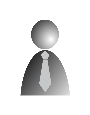
\includegraphics{./logos/decider-220x320.eps}};
  
% TOP DOWN linkings of the component IO structure:  
\draw[->,Gray] (Composer) to [out=270,in=90] (FRONTEND);
\draw[->,Gray] (FRONTEND) to [out=270,in=90] (FOUT);
\draw[->,Gray] (FOUT) to [out=270,in=90] (CONVERTER);
\draw[->,\mtexColor] (CONVERTER) to [out=270,in=90] (BIN);

\draw[->,\mtexColor] (BIN) to [out=270,in=90] (BACKEND);
\draw[->,Gray] (BACKEND) to [out=270,in=90] (PDF);

\end{tikzpicture}
\end{center}

Die verschiedenen Aufgaben solcher Systeme auseinanderzuhalten, ist bei der
Begutachtung von Lösungen essentiell. So attestiert z.B. eine ältere Sichtung
von Notensatzprogrammen der \enquote{Open Source Welt}, sie habe
\enquote{[\ldots] noch immer Schwierigkeiten, ein [\ldots] Nischenprodukt wie
ein Notensatzprogramm zu entwickeln}. Und sie begründet ihr Urteil damit, dass
\enquote{[\ldots] eine neue Mark-up-Sprache zu erlernen und in dieser grafische
Vorstellungskraft zu entwickeln [\ldots] nicht jedermanns Sache (sei)}, auch
wenn die Ergebnisse -- wie im Falle von \acc{Frescobaldi} und \acc{LilyPond} --
\enquote{[\ldots] äußerst professionell anmuten
(mögen)}.\footcite[vgl.][51]{Albrecht2009a} Wenn man, wie hier geschehen,
(graphische) Editoren und eigentliche Notensatzprogramme implizit 'gleichsetzt',
dann beraubt man sich der Möglichkeit zu einem differenzierteren und
pragmatischen Urteil: Wer integrierte Gesamtsysteme erwartet, bewertet komplexe
Architekturen mit verteilten Teilsystem eben dieser Verteilung wegen schlechter
-- und verkennt, das sehr viel komplexere Systeme nach diesem Prinzip aufgebaut
sind und erfolgreich betrieben werden, wie etwa \acc{Unix} resp.
\acc{GNU/Linux}.

Wir jedenfalls werden diesen Aspekten gesondert nachgehen: Zuerst analysieren
wir mögliche 'Backends' und deren Methoden, 'Noten' in \LaTeX-Texte einzubinden.
Sie sind insofern \acc{Backends}, als sie textuellen Input verarbeiten, der auch
über vorgelagerte, eher graphische Programme erzeugt werden könnte. Diese bilden
das 'Frontend' für den Arrangeur, Komponisten oder Musikwissenschafter. Solche
graphischen und semi-graphische Editoren und Konverter werden wir anlysieren,
nachdem die Backends begutachtet haben. Und ganz am Ende werden wir sehen, dass
uns gerade diese Aufteilung eine besondere Flexibilität bietet, Notenbeispiele
in (musik)wissenschaftliche Arbeiten einzubetten.

Allerdings werden wir uns bei unser Betrachtung auf die Open-Source-Welt
konzentrieren. Mehr oder minder konstenintensive proprietäre Programme mögen
beliebt sein, notwendig sind sie nicht. Es ist auch für den Musiker besser,
nicht in die 'Vendorenfalle' zu geraten und seine Arbeiten von den Produkten
einer Firma abhängig zu machen. Deshalb fokussieren wir uns hier auf die
Umsetzung mit freier Software.\footnote{Wer als Musiker proprietäre Programme
nutzt, macht sich erpressbar: Auf der einen Seite investiert er Zeit und Mühen
in die Erstellung von Notentexten, die er (darum) auch später noch
weiterverarbeiten oder wiederverwenden will. Auf der anderen Seite muss er
fürchten, die hinter dem eigenen Programm stehende Firma werde beim nächsten
Versionswechsel die Lizenzgebühren so stark erhöhen, dass sie sein Budget
sprengen. Und selbst ohne diese finale Katastrophe wird der Wechsel zu einem
anderen Anbieter mit der Zeit durch die schon investierte Arbeit so aufwendig,
dass man lieber bei dem bisherigen Programm bleibt, auch wenn es teuerer oder
schlechter ist als die Alternativen. Damit ist man in die \textit{Vendorenfalle}
getappt. Mit freier Software kann das nicht geschehen, weil es zum Wesen freier
Software gehört, dass man ohne pekuniären Aufwand an den Quellcode und an die
Nutzungsrechte der ablauffähigen Programme herankommt - auch an die neuerer und
besserer Versionen. (\cite[vgl. dazu][\nopage wp.]{FSF2018a}.) Für Musiker hat
sich die Lage mit der Etablierung von \textit{MusicXML} allerdings etwas
entspannt: Durch die Standardisierung des Dateiformates wird der Wechsel zu
einem anderen, besseren Programme erleichtert. Hier muss man 'nur' noch
fürchten, dass das bisher die jeweiligen Programme vorab (noch) nicht
standardisierte Features benutzen oder den Standard nicht ganz konform
implementiert haben. Allerdings sind solche 'Eigenarten' ein beliebtes Mittel
der Entwickler, den zahlenden Kunden zuletzt doch wieder an sich zu binden und
ihm den Wechsel zur Alternative zu erschweren. (\cite[Zur Lizenzierung von
MusicXML vgl. auch][\nopage wp.]{WpedMusicXML2018a}) Dieser Kontext gibt uns
auch die Gelegenheit, auf die Lizenzproblematik einzugehen: Wir werden bei den
Tools jeweils kurz nachweisen, dass es es sich tatsächlich um freie Software
bzw. Open Source Software handelt. Dass dem so ist, ist uns wichtig. Denn aus
einem solchen Nachweis ergibt sich, dass man die Software ohne Einschränkungen
und unentgeltlich nutzen darf. Allerdings folgt Open Source Software dem Prinzip
'Paying by Doing'. Anstatt -- wie sonst üblich -- die Nutzungsrechte zu kaufen,
'erwirbt' man diese, indem man das aktiv tut, was die Lizenzen dem Nutzer
auftragen. Zu wissen, was das ist, ist kein Hexenwerk, kann in Einzelfällen aber
'tricky' werden. Diese rechtlichen Rahmenbedingungen sind nicht unser Thema. Wir
gehen deshalb davon aus, dass Sie sich selbst darum kümmern werden, wenn es
angesagt ist. Unser Erfahrung nach gibt es dafür eine gute Daumenregel: Sie
dürfen die Frage, ob und wie sie die Software lizenzkonformen nutzen, solange
aufschieben, bis Sie sich entscheiden, die Software an andere weiterzugeben.
Oder anders gesagt: Solange Sie selbst diese Software 'nur' von irgendwoher
downgeloaded oder installiert haben und anwenden, solange dürfen Sie die
Beachtung der Compliance auch 'gefahrlos' auf später verschieben.}

Dazu noch einige abgrenzende Worte:
\begin{itemize}
  \item Damit Sie einen guten Gewinn von der Lektüre haben, sollten Sie mit der
  Nutzung von \LaTeX\ unter Ihrem Betriebssystem vertraut sein.
  Insbesondere die Erweiterung Ihres \TeX-Systems und die Installation von
  zusätzlichen CTAN-Paketen legen wir kommentarlos in Ihre Hände\footnote{Es
  gibt eine Fülle guter, auch auf die Praxis ausgerichteter \LaTeX-Einführungen.
  (\cite[etwa][7ff]{Schlosser2016a}). Die ma\-nuelle Installation eines
  CTAN-Paketes ist -- wenn überhaupt nötig -- so schwierig nicht: Man lädt sich das
  Paket herunter und entpackt es in einem Ordner. Dann kopiert man diesen Ordner
  -- nötigtenfalls mit Root-Rechten -- in die \LaTeX-Distribution, z.B. unter
  \texttt{/usr/share/texmf/tex/latex/} (wobei \acc{/usr/share/texmf}
  distributionsabhängig ist). Und schließlich setzt man an der Konsole / im
  Terminal noch einmal das Kommando \texttt{sudo texhash} ab, um das neue Paket
  bekannt zu machen. Wenn Sie eine gängige Distribution benutzen, sollte der
  Rückgriff auf solch eine Detailarbeit aber gar nicht nötig sein.}.
  \item Ferner setzen wir voraus, dass Sie die Tools und Programme, die wir
  erwähnen, unter Ihrem Betriebssystem installieren können.
  \item Außerdem werden wir Sie nicht anleiten, wie man mit einem der
  begutachteten System Notentexte schreibt. Dazu gibt es bessere und genauere
  Handbücher, auf die wir gerne und dankbar verweisen. Was wir Ihnen jedoch
  zeigen werden, ist, wie man die mit den Tools erarbeitete Notentexte - wenn
  überhaupt möglich - in einen \LaTeX-basierten wissenschaftlichen Text
  integriert.
  \item Und schließlich gehen wir ohne große Prüfung davon aus, dass die
  Programme und Tools, die behaupten, für verschiedene Betriebssysteme zu
  existieren, im wesentlichen gleich funktionieren. In der Open-Source-Welt ist
  dem üblicherweise so.
\end{itemize}

Und damit wollen wir es gut sein lassen mit dem Erwartungsmanagement.



% this is only inserted to eject fault messages in texlipse
%\bibliography{../bib/literature}


% mycsrf 'for beeing included' snippet template
%
% (c) Karsten Reincke, Frankfurt a.M. 2012, ff.
%
% This text is licensed under the Creative Commons Attribution 3.0 Germany
% License (http://creativecommons.org/licenses/by/3.0/de/): Feel free to share
% (to copy, distribute and transmit) or to remix (to adapt) it, if you respect
% how you must attribute the work in the manner specified by the author(s):
% \newline
% In an internet based reuse please link the reused parts to mycsrf.fodina.de
% and mention the original author Karsten Reincke in a suitable manner. In a
% paper-like reuse please insert a short hint to mycsrf.fodina.de and to the
% original author, Karsten Reincke, into your preface. For normal quotations
% please use the scientific standard to cite
%


%% use all entries of the bibliography

\subsection{Kriterien}

Wer den besten Weg sucht, braucht Maßstäbe. Deshalb werden wir den
Notensatzsystemen drei Referenzkadenzen vorlegen und erwarten, dass sie diese
optisch ansprechend erfassen und wiedergeben können, und zwar einschließlich der
zugehörigen Harmonieanalyse:

Als erste und einfachste Aufgabe beziehen wir uns auf ein Beispiel aus der
Harmonielehre von Grabner\footcite[vgl.][107]{Grabner1974a}:

\begin{center}
\begin{music}%
  \largemusicsize%
  % using defaults: \instrumentnumber{1}% + \setstaffs{1}{1}  
  % + \setclef{1}{\treble}+ no bar type + \generalsignature{0}%
  \nobarnumbers%
  \startextract%
  \setdoublebar%
  \NOTEs\lcharnote{10}{(1) }\uptext{T}\zchar{-10}{I}\zw{ce}\wh{g}\en%
  \NOTEs\uptext{S}\zchar{-10}{IV}\zw{fh}\wh{j}\en%
  \NOTEs\uptext{D}\zchar{-10}{V}\zw{gi}\wh{k}\en%
  \bar%
  \NOTEs\lcharnote{10}{(2) }\uptext{T}\zchar{-10}{I}\zw{ac}\wh{e}\en% 
  \NOTEs\uptext{S}\zchar{-10}{IV}\zw{df}\wh{h}\en%
  \NOTEs\uptext{D}\zchar{-10}{{I}}\sh{g}\zw{eg}\wh{i}\en%
  \setdoublebar%
  \endextract%
\end{music}%
\cad{I}{Referenz}
\end{center}

Die zweite Referenzkadenz soll die Erfassung harmonisch komplexer Zusammenhänge
abfordern:

\begin{center}
\begin{music}
  \normalmusicsize
  \parindent4em
  \instrumentnumber{1}
  \setstaffs{1}{2}
  \setclef{2}{\treble}
  \setclef{1}{\bass}
  \setname{1}{Piano}
  \generalsignature{2}% D-DUR
  \generalmeter{\meterfrac42}
  \startextract
  \NOTes\zmidstaff{\HH.T.....}\zh{K}\hl{a}|\zh{f}\hu{k}\en%
  \NOTes\zmidstaff{(\HH.D..7...)}\zh{I}\hl{a}|\zh{f}\sh{k}\hu{k}\en%
  \NOTes\zmidstaff{\HH.Sp.7...7.}\zh{K}\hl{N}|\zh{i}\hu{l}\en%
  \NOTes\zmidstaff{\HH.\Dohne.3.$\flat$9=$\sharp$8.7.5.}\zh{J}\hl{N}|\zh{i}\sh{l}\hu{l}\en%
  \bar
  \NOTes\zmidstaff{\HH.Tp.3....}\zh{K}\hl{M}|\zh{i}\hu{m}\en%  
  \NOTes\zmidstaff{\HH.\DD.5...7.}\zh{I}\hl{K}|\zh{l}\sh{n}\hu{n}\en%  
  \NOTes\zmidstaff{\HH.D....4-3.}
    \zh{H}\isluru{0}{K}\qu{K}\tslur{0}{J}\qu{J}|
    \zhl{l}\hl{o}\en%  
  \NOTes\zmidstaff{\HH.T.....}\zh{D}\hl{K}|\zh{m}\hu{o}\en%  
  \setdoublebar
  \endextract
\end{music}
\cad{II}{Referenz}
\end{center}

Und die dritte Referenzkadenz soll das in einen schwierigeren
rhythmish-metrischen Kontext einbetten:

\begin{music}
  \smallmusicsize
  \parindent4em 
  \instrumentnumber{2}
  \setstaffs{2}{1}
  \setstaffs{1}{1}
  \setclef{2}{\treble}
  \setclef{1}{\bass} 
  \songtop{2} 
  \songbottom{1} 
  \setname1{Bass}
  \setname2{Diskant}
  \generalsignature{-2}
  \generalmeter{\meterfrac58}
  \startpiece
    % Takt 1/1: B: 2 8tel (Kurzschreibweise) + D: 4tel AKK
    \NOtes \zmidstaff{T} \Dqbl I b & \zq{ik}\qu{m}\en
    % Takt 1/3: B: 2 8tel explizit  mit Vorzeichen + D: 4etl AKK
    \NOtes \zmidstaff{\HH.D.3-3$\flat$.8.7..} 
      \ibl{0}{a}{0}\qb{0}{a}\tbl{0}\fl{a}\qb{0}{a} & 
      \zq{j}\rq{l}\qu{m} \en
    % Takt 1/5: B: punktierte 16tel explizit mit Vorzeichen + D: 8tel AKK
    \NOtes \zmidstaff{\HH.S.3-3$\flat$....} 
      \ibbl{2}{N}{0}\qbp{2}{N}\roff{\tbbbl{2}\fl{N}\tqb{2}{N}} & 
      \zq{il}\cu{p}\en
  \bar % T2: 2*(B:2*8. + D:4. AKK) +  B:2*16. + D:8. AKK
    \NOtes \zmidstaff{\HH.D.8-7.7...} 
      \Dqbl M L &  \zq{jl}\qu{o} \en
    \NOtes \zmidstaff{\HH.Dp.8-8$\flat$....} 
      \ibl{1}{K}{0}\qbp{1}{K}\roff{\tbbl{1}\fl{K}\tqb{1}{K}} & 
      \zq{hm}\qu{o}\en
    \NOtes \zmidstaff{\HH.D.5-3.7...}
      \ibbl{2}{J}{0}\qbp{2}{J}\roff{\tbbbl{2}\tqb{2}{H}} & 
      \zq{j}\rq{l}\cu{m} \en
  %\alaligne
  \bar %T3 B:8. + D:8. P + B:8. P + D:8.AKK + B:8. + D:8.AKK + B:4. + D:4.AKK 
    \notes \zmidstaff{T} \qa I & \ds \zq{fk}\cu{m}\en
    \notes \zmidstaff{\HH.D..7...} \ca M & \zq{eh}\cu{j}\en
    \notes \zmidstaff{T} \qa b & \zq{df}\qu{i}\en
  \bar %T4: 8. P + (B:2*8. + D:4. AKK) + B:8. + D:8.AKK + 8. P 
    \notes \ds & \ds \en
    \notes \zmidstaff{\HH.D..7...} \ca{M J} & \zq{eh}\qu{j}\en
    \notes \qa F & \zq{eh}\qu{j}\en  
  \bar %T5: 8. P + 2*(B:8. + D:8. AKK) + 8. P +  B:8. + D:8.AKK  
    \notes \ds & \ds \en
    \notes \zmidstaff{\HH.D..7...} \ca M & \zq{eh}\cu{j}\en
    \notes \zmidstaff{\HH.D.3.7...} \ca H & \zq{j}\rq{l}\cu{m}\en
    \notes \zmidstaff{T} \qa I & \zq{ik}\qu{m}\en  
  \bar % T6: 3*(B:8.  + D:8. AKK) + B:4. + D:4. AKK
    \notes \ds & \ds \en
    \notes \zmidstaff{\HH.S..5.6..}  \ca L & \zq{g}\rq{i}\cu{j}\en
    \notes \zmidstaff{\HH.D..7...} \ca M & \zq{eh}\cu{j}\en  
    \notes \zmidstaff{T} \qa b & \zq{df}\qu{i}\en    
  \Endpiece
\end{music}
\cad{III}{Referenz}

Zuletzt werden wir dann -- wie angekündigt -- versuchen, nach guten Frontends
für die \LaTeX-kompatiblen Notensatzsysteme suchen, nach Editoren. Von ihnen
werden das verlangen, was wir auch von den Konvertern erwarten, dass sie nämlich
die Referenzkadenz II erfassen und adäquat exportieren. Wie wir verifizieren
werden, dass eine Refrenzkadenz adäquat exportiert bzw. konvertiert worden ist,
werden wir später genauer noch erläutern.\footnote{$\rightarrow$ S.
\pageref{ExportVerifikation}}

% this is only inserted to eject fault messages in texlipse
%\bibliography{../bib/literature}


\section{Leichtgewichtige Teillösungen}

Selbstverständlich wird sich zuletzt herausstellen, dass adäquate Systeme zur
Erfassung von Musik eine gewisse Komplexität mitbringen. Das liegt in der Natur
der Sache: Musik ist zweidimensional.\footnote{Bei der Notation von Musik hatten
wir gesagt, dass sie zweidimensional oder eindimensional codiert sein könne.
Als Abfolge(sic!) von Klängen(sic!) ist sie selbst aber immer (mindestens)
zweidimensional.} Das hat einige Autoren nicht entmutigt, wenigstens für
Teilaufgaben einfachere Lösungen zu entwickeln, die im freien Textsatzsystem
\LaTeX\footnote{Bzgl. der Zusammenhänge von \TeX, \LaTeX, pdf\LaTeX\ und
Lua\LaTeX\ vlg. etwa \cite[][7ff]{Voss2018a} oder \cite[][8ff]{Voss2012a}.
Daraus ergibt sich mittelbar auch der Open-Source-Status von \LaTeX: \TeX\ und
\LaTeX\ sind zunächst einmal 'nur' eine Metasprache. Um aus Dateien, die in
dieser Auszeichnungssprache formuliert sind, typographisch gestaltete \acc{DVI}-
oder \acc{PDF}-Dateien zu erzeugen, bedarf des bestimmter Programme, nämlich
\texttt{pdflatex}, \texttt{lualatex}\ etc. Außerdem hat sich um \LaTeX\ herum ein
Biotop von Paketen entwickelt. Das sind fertig vorbereitete \TeX- oder
\LaTeX-Dateien, die man in seine eigenen Dokumente einbindet und also mitnutzt.
Solche Pakete stehen -- mit den Kernprogrammen gebündelt -- als komplette
\TeX-Distributionen bereit. Für den europäischen Raum existieren z.Zt. zwei
wesentliche Distributionen, \acc{{\TeX}live} und \acc{MiK{\TeX}}. Diese findet
man im \acc{Comprehensive TeX Archive Network} ($\rightarrow$
\href{https://ctan.org/}{https://ctan.org/}). Der unbedarfte Anwender tut aber
gut daran, sich vorbereitete Installationspakete von sekundären Distributoren zu
holen. \acc{Linux}-Distributionen liefern diese i.d.R. mit. Ob man sein
\LaTeX-System lizenzkonform nutzt, entscheidet also die Lizensierung der
Kernprogramme und die Lizenzen der eingebundenen Pakete. Diese müssen nicht
unter derselben Lizenz veröffentlicht sein. Glücklicherweise werden beide -- die
Kernprogramme und die Erweiterungen -- als \acc{CTAN}-Pakete gehostet und unter
den Bedingungen verschiedener FOSS-Lizenzen zum Download angeboten. So ist etwa
pdf\LaTeX\ unter der GPL lizenzisiert ($\rightarrow$
\href{https://ctan.org/pkg/pdftex} {https://ctan.org/pkg/pdftex}). Ganz
allgemein gesagt, darf man alles, was zu \LaTeX\ gehört, als freie Software
nutzen. Wir werden bei den Paketen jedoch kurz angeben, unter welcher Lizenz sie
genau stehen.} genutzt werden können.
Diesen werden wir zuerst nachgehen. Behalten wir aber im Hinterkopf:
\acc{Komplexität ist wie Wasser, man kann es nicht
komprimieren.}\footnote{Dieses wunderbare Bonmot stammt nicht von mir. Und
bedauerlicherweise weiß ich auch nicht (mehr) von wem. Ich meine es etwa Anfang
der 2010er Jahre in einer Keynote bei der Deutschen Telekom in Darmstadt gehört
zu haben. Ich verbeuge mich also dankbar vor dem mir leider unbekannten Autor.}


% mycsrf 'for beeing included' snippet template
%
% (c) Karsten Reincke, Frankfurt a.M. 2012, ff.
%
% This text is licensed under the Creative Commons Attribution 3.0 Germany
% License (http://creativecommons.org/licenses/by/3.0/de/): Feel free to share
% (to copy, distribute and transmit) or to remix (to adapt) it, if you respect
% how you must attribute the work in the manner specified by the author(s):
% \newline
% In an internet based reuse please link the reused parts to mycsrf.fodina.de
% and mention the original author Karsten Reincke in a suitable manner. In a
% paper-like reuse please insert a short hint to mycsrf.fodina.de and to the
% original author, Karsten Reincke, into your preface. For normal quotations
% please use the scientific standard to cite
%


%% use all entries of the bibliography

\subsection{Sonderzeichen: der Standard ($\bigstar\bigstar\bigstar$)}

Neben Zeichen für die Schriftsprache als solche bot \LaTeX\ - der
Mathematik sei Dank - immer schon auch graphische Symbole an, die wie
Schriftzeichen in einer Zeile platziert werden können.\footcite[vgl.][543ff et
passim]{MitGoo2005a} Sie werden im Mathematikmodus notiert, haben also die Form
\texttt{\small \$\textbackslash{ZEICHENNAME}\$}. Und in diesem Fundus von Sonderzeichen
gibt es auch die drei Symbole $\sharp$ (= \texttt{\small \$\textbackslash{sharp}\$}),
$\flat$ (= \texttt{\small \$\textbackslash{flat}\$}) und $\natural$ (=
\texttt{\small \$\textbackslash{natural}\$}).

Diese Zeichen können ohne Zusatzpaket in einem \LaTeX-Quelltext genutzt
werden. Unnötig zu erwähnen, dass sie -- für sich genommen -- nicht ausreichen,
Musik textuell zu erfassen. Dennoch wird man in der Kombination mit anderen
Ansätzen gelegentlich auf sie zurückkommen wollen.\footnote{In diesem
Zusammenhang wäre auch zu erwähnen, dass Unicode und seine Encodierung UTF-8 von
sich aus einen Bereich mit 'Musikzeichen' definiert hat, nämlich die Zeichen
zwischen \texttt{U+1D100} und \texttt{U+1D1FF} (\cite[Vgl. dazu][\nopage
wp.]{Koellerwirth2015a}). Wenigstens unter (pdf)\LaTeX. bedarf Nutzung dieser
Zeichen -- wenn überhaupt möglich -- zusätzlicher Maßnahmen. (\cite[Zum
Zusammenhang zwischen Unicode und UTF( vgl.][\nopage wp.]{Kuhn2019a})}

% this is only inserted to eject fault messages in texlipse
%\bibliography{../bib/literature}


% mycsrf 'for beeing included' snippet template
%
% (c) Karsten Reincke, Frankfurt a.M. 2012, ff.
%
% This text is licensed under the Creative Commons Attribution 3.0 Germany
% License (http://creativecommons.org/licenses/by/3.0/de/): Feel free to share
% (to copy, distribute and transmit) or to remix (to adapt) it, if you respect
% how you must attribute the work in the manner specified by the author(s):
% \newline
% In an internet based reuse please link the reused parts to mycsrf.fodina.de
% and mention the original author Karsten Reincke in a suitable manner. In a
% paper-like reuse please insert a short hint to mycsrf.fodina.de and to the
% original author, Karsten Reincke, into your preface. For normal quotations
% please use the scientific standard to cite
%


%% use all entries of the bibliography

\subsection{Andere Sonderzeichen: wasysym}

Gleiches gilt für das \LaTeX-Zusatzpaket \textit{wasysym}\footcite[vgl.][\nopage
wp]{CtanWasysym2018a}: Es erweitert den Vorrat an musikalischen Zeichen um
einige Notensymbole. Wie in \LaTeX\ üblich, muss das Paket über ein Kommando in
die Präambel eingebunden werden
(\texttt{\textbackslash{usepackage\{wasysym\}}}), damit man anschließend auf die
Zeichen \eighthnote \ (= \texttt{\small \textbackslash{eighthnote}}),
\quarternote \ (= \texttt{\small \textbackslash{quarternote}}), \halfnote \ (=
\texttt{\small \textbackslash{halfnote}}), \fullnote \ (= \texttt{\small
\textbackslash{fullnote}}), und \twonotes \ (= \texttt{\small
\textbackslash{twonotes}}) zugreifen kann\footcite[vgl.][2]{Kielhorn2003a}.


 
% mycsrf 'for beeing included' snippet template
%
% (c) Karsten Reincke, Frankfurt a.M. 2012, ff.
%
% This text is licensed under the Creative Commons Attribution 3.0 Germany
% License (http://creativecommons.org/licenses/by/3.0/de/): Feel free to share
% (to copy, distribute and transmit) or to remix (to adapt) it, if you respect
% how you must attribute the work in the manner specified by the author(s):
% \newline
% In an internet based reuse please link the reused parts to mycsrf.fodina.de
% and mention the original author Karsten Reincke in a suitable manner. In a
% paper-like reuse please insert a short hint to mycsrf.fodina.de and to the
% original author, Karsten Reincke, into your preface. For normal quotations
% please use the scientific standard to cite
%


%% use all entries of the bibliography

\subsection{Noch mehr Sonderzeichen: musicography ($\bigstar\bigstar$)}

Das Zusatzpaket \acc{musicography}\footnote{\cite[vgl.][\nopage
wp]{CtanMusicography2018a}. Die Paketbeschreibung gibt an, dass
\acc{musicography} unter der \acc{LaTeX\ Project Public Li­cense} veröffentlicht
wird. Das ist eine von der \acc{OSI} anerkannte Open-Source-Lizenz
($\rightarrow$ \href{https://opensource.org/licenses/LPPL-1.3c}
{https://opensource.org/licenses/LPPL-1.3c}).} vereinigt und erweitert die
bisher erwähnten Möglichkeiten. Außerdem sagen manche Fürsprecher, dass es -- im
Gegensatz zu anderen Paketen -- auch mit \textit{pdflatex} druckfähige
PDF-Dateien erzeuge.\footnote{\cite[Vgl. dazu etwa][1]{Cashner2018a}. Persönlich
sind uns bei der PDF-Generierung solche Irritationen mit anderen Paketen nicht
begegnet. \acc{mycsrf} nutzt auch \textit{pdflatex}. Und unter Ubuntu 18.04
werden dabei alle Fonts eingebunden und können alles ausdrucken, was auch am
Bildschirm sichtbar ist: so auch bei dem Beispiel \textit{musicology.de}.}
Selbstverständlich muss auch dieses \LaTeX-Paket in die Präambel des
\LaTeX-Dokumentes eingebunden werden (\texttt{\small
\textbackslash{usepackage\{musicography\}}}), um entsprechende Befehle nutzen zu
können.

Anschließend erlaubt das Paket, Vorzeichen \{
\musFlat \ (= \texttt{\small \textbackslash{musFlat}}),
\musSharp \ (= \texttt{\small \textbackslash{musSharp}}),
\musNatural \ (= \texttt{\small \textbackslash{musNatural}}),
\musDoubleFlat \ (= \texttt{\small \textbackslash{musDoubleFlat}}),
\musDoubleSharp \ (= \texttt{\small \textbackslash{musDoubleSharp}})
\}, Notensymbole \{
\musWhole \ (= \texttt{\small \textbackslash{musWhole}}),
\musHalf \ (= \texttt{\small \textbackslash{musHalf}}),
\musQuarter \ (= \texttt{\small \textbackslash{musQuarter}}),
\musEighth \ (= \texttt{\small \textbackslash{musEighth}}),
\musSixteenth \ (= \texttt{\small \textbackslash{musSixteenth}}),
\musHalfDotted \ (= \texttt{\small \textbackslash{musHalfDotted}}),
\musQuarterDotted \ (= \texttt{\small \textbackslash{musQuarterDotted}})
\ldots
\}
und Metren wie \meterCutC \ (= \texttt{\small \textbackslash{meterCutC}})
in den Fließtext einzuarbeiten.

Gleichwohl gibt es dabei einige 'Ungereimtheiten', die den Gebrauch erschweren:
\begin{itemize}
  \item Zum ersten muss man das Paket \textit{MusiX\TeX}, sofern man es zusammen
  mit \textit{musicology} verwenden will, nach \textit{musicology} in die Präambel
  einbinden. Andernfalls 'meckert' \textit{musicology}, dass der Befehl
  \texttt{meterC} schon definiert sei. Bindet man \textit{MusiX\TeX} tatsächlich
  nach \textit{musicology} ein, kann \textit{MusiX\TeX} den von \textit{musicology}
  eingeführten Befehl offensichtlich problemlos redefinieren. Leider passen die
  Symbole dann -- wie man hier sehen kann -- von der Größe her nicht mehr zu
  einander: \textit{musicology} $\rightarrow$ \meterCutC : \meterC $\leftarrow$
  \textit{MusiX\TeX}.
  \item Außerdem sind die Symbole für die Achtel- (\musEighth) und die
  Sechzehntelnoten (\musSixteenth) aus Musikersicht unbrauchbar. Solche Zeichen
  gibt es in der Musik(wissenschaft) nicht.
\end{itemize}

Wenn man dieses Paket verwenden will, ist also eine gewisse Vorsicht angesagt.


% this is only inserted to eject fault messages in texlipse
%\bibliography{../bib/literature}


% mycsrf 'for beeing included' snippet template
%
% (c) Karsten Reincke, Frankfurt a.M. 2012, ff.
%
% This text is licensed under the Creative Commons Attribution 3.0 Germany
% License (http://creativecommons.org/licenses/by/3.0/de/): Feel free to share
% (to copy, distribute and transmit) or to remix (to adapt) it, if you respect
% how you must attribute the work in the manner specified by the author(s):
% \newline
% In an internet based reuse please link the reused parts to mycsrf.fodina.de
% and mention the original author Karsten Reincke in a suitable manner. In a
% paper-like reuse please insert a short hint to mycsrf.fodina.de and to the
% original author, Karsten Reincke, into your preface. For normal quotations
% please use the scientific standard to cite
%


%% use all entries of the bibliography


\subsubsection{Das harmony-Paket: ein echtes Highlight}

Das Paket \emph{harmony}\footcite[vgl.][\nopage wp]{CtanHarmony2018a} bietet für
den Gebrauch innerhalb einer Textzeile ein besonders ausgefeiltes System von
Musikzeichen an. Als \LaTeX-Paket muss es natürlich ebenfalls zuerst mittels
eines Befehls in die Präambel eingebunden werden (\small 
\texttt{\textbackslash{usepackage\{harmony\}}}), bevor es Zeichen für die beiden
Bereiche \emph{Rhythmik} und \emph{Harmonieanalyse} bereitstellt\footcite[Für
einen vollen Überblick über den Zeichenvorrat und die Kombinationsmöglichkeiten
vgl.][4ff]{WegWeg2007a}:

\paragraph{\small Rhythmik}$\;$ \\

Zunächst enthält es gut funktionierende Encodierungen für Taktarten \{ 
\Takt{3}{4} \ (= \texttt{\small \textbackslash{Takt}\{3\}\{4\}}),
\Takt{4}{4} \ (= \texttt{\small \textbackslash{Takt}\{4\}\{4\}}),
\ldots,
\Takt{c}{0} \ (= \texttt{\small \textbackslash{Takt}\{c\}\{0\}}),
\Takt{c}{1} \ (= \texttt{\small \textbackslash{Takt}\{c\}\{1\}})
\}.
Dann offeriert es nicht nur einfache Notenlängen \{
\Ganz \ (= \texttt{\small \textbackslash{Ganz}}),
\Halb \ (= \texttt{\small \textbackslash{Halb}}),
\Vier \ (= \texttt{\small \textbackslash{Vier}}),
\Acht \ (= \texttt{\small \textbackslash{Acht}}),
\Sech \ (= \texttt{\small \textbackslash{Sech}}),
\Zwdr \ (= \texttt{\small \textbackslash{Zwdr}}),
\}  -- \ die sogar punktiert werden können 
\{
\Halb\Pu \ (= \texttt{\small \textbackslash{Halb}\textbackslash{Pu}}),
\Vier\Pu \ (= \texttt{\small \textbackslash{Vier}\textbackslash{Pu}}),
\ldots
\}
-- ,
sondern es stellt die Symbole auch mit waagerechten Balken zu Verfügung
\{
\AchtBL \ (= \texttt{\small \textbackslash{AchtBL}}),
\SechBL \ (= \texttt{\small \textbackslash{SechBL}}),
\Vier\AchtBL \ (= \texttt{\small \textbackslash{Vier} \textbackslash{AchtBL} }),
\Vier\SechBL \ (= \texttt{\small \textbackslash{Vier} \textbackslash{SechBL} }),
\ldots
\}, 
sodass die einzelnen Elemente zu ganzen Rhythmusketten kombiniert werden können: 
\Takt{c}{0} \Vier \ \Vier\AchtBL \ \Vier\Pu \ \Acht \ $|$ 
\AchtBR\Pu \SechBl \ \AchtBR\kern-0.15em\SechBR\Vier \ \SechBr\Vier\SechBl \ $|$
\ -- eine wirklich ausgefuchste Lösung.

\paragraph{\small Harmonik}$\;$ \\

Einen ähnlich geschickten Ansatz bietet das Paket \emph{harmony} da, wo es
Symbole erzeugt, die -- der Funktions- und Stufentheorie entsprechend --
harmonische Zusammenhänge repräsentieren.

Den Kern bildet die allgemeine Tupelkonstruktion \texttt{\small
\textbackslash{HH.X.u.v.w.z.}}, mit der einfache und komplexe Aspekte
dargestellt werden können\footcite[vgl. dazu][2ff]{WegWeg2007a}: Was zwischen
den ersten beiden Punkten erscheint (X), erscheint als Hauptzeichen; dann folgt
das, was darunter erscheinen soll (u) und schließlich das, was rechts oben
daneben angezeigt werden soll, und zwar von oben nach unten (v w z):

\begin{center}
\HH.X.u.v.w.z.
\end{center}

Der Witz ist nun, dass man nahezu beliebige Latexkonstrukte zwischen den Punkten
einsetzen kann. Und wenn man nichts zwischen den Punkten einträgt, bleibt der
Platz leer. So können die einfachen Symbole der Funktionstheorie \{ \HH.T..... 
\ (= \texttt{\small \textbackslash{HH.T.....}}), \HH.Tp.....  \ (=
\texttt{\small \textbackslash{HH.Tp.....}}), \HH.S.....  \ (= \texttt{\small
\textbackslash{HH.S.....}}), \HH.D.....  \ (= \texttt{\small
\textbackslash{HH.D.....}}) \} ebenso erzeugt werden, wie komplexere \{
\HH.D.3.9.7..  \ (= \texttt{\small \textbackslash{HH.D.3.9.7..}}),
\HH.T..9\VM-8.7..  \ (= \texttt{\small \textbackslash{HH.T..9\VM-8.7..}}) \}.
Die speziellen Zeichen der Funktionstheorie, die nicht so einfach aus dem Fundus
normaler Fonts gebildet werden können, stellt  \emph{harmony} gesondert zur
Verfügung:
\{ \Dohne  \ (= \texttt{\small \textbackslash{Dohne}}), \DD \ (= \texttt{\small
\textbackslash{DD}}), \DS  \ (= \texttt{\small \textbackslash{DS}}) \}.
Selbstverständlich können diese ebenfalls in das allgemeine Tupelkonstrukt
eingebettet werden\footcite[Vgl. dazu][6]{WegWeg2007a}:
\begin{center}
 \texttt{\textbackslash{HH}.\textbackslash{DD}.5\textbackslash{VM}.7...} 
 $\rightarrow$ \HH.\DD.5\VM.7...
\end{center}

Zudem erlaubt es die Flexibilität des Grundkonstruktes (in gewissen Grenzen),
Symbole für die Stufentheorie und den Generalbass zu erzeugen:

\begin{center}
\HH.I..\texttt{(5)}.\texttt{(3)}.. \ 
\HH.III..\texttt{ 6 }.\texttt{(3)}.. \ 
\HH.V..\texttt{ 6}.\texttt{ 4}.. \ 
\HH.I..\texttt{(5)}.\texttt{(3)}.. \ 
\HH.I..\texttt{(5)}.\texttt{ 3$\flat$ }.. \ 
\HH.III..\texttt{ 6 }.\texttt{ 3$\flat$}.. \ 
\HH.III..\texttt{ 6 }.\texttt{ 5 }.\texttt{(3)}. \ 
\HH.III..\texttt{ 6$\flat$}.\texttt{ 3$\flat$}.. \ 
\end{center}

Man sieht an diesem Beispiel auch, dass sich die \emph{harmony}-Konstrukte (hier
\texttt{\textbackslash{texttt}} und \texttt{\$\textbackslash{flat}\$} ) gut mit
anderen \LaTeX-Elementen kombinieren lassen:
\begin{verbatim}
\begin{center}
\HH.I..\texttt{(5)}.\texttt{(3)}.. \ 
\HH.III..\texttt{ 6 }.\texttt{(3)}.. \ 
\HH.V..\texttt{ 6}.\texttt{ 4}.. \ 
\HH.I..\texttt{(5)}.\texttt{(3)}.. \ 
\HH.I..\texttt{(5)}.\texttt{ 3$\flat$ }.. \ 
\HH.III..\texttt{ 6 }.\texttt{ 3$\flat$}.. \ 
\HH.III..\texttt{ 6 }.\texttt{ 5 }.\texttt{(3)}. \ 
\HH.III..\texttt{ 6$\flat$}.\texttt{ 3$\flat$}.. \ 
\end{center}
\end{verbatim}

Später werden wir zeigen, dass sich die \emph{harmony}-Elemente ihrerseits
auch gut in MusiX\TeX-Syntagmen einbetten lassen. Insofern haben die
Programmierer von \emph{harmony} der Community ein mächtiges Werzeug zur
Verfügung gestellt\footnote{Trotzdem wollen auch wir wenigstens darauf
hinweisen, dass \emph{harmony}-Konstrukten auf die Einbettung in einen Fließtext
mit 12 Pt. ausgelegt sind. Bei kleineren Größen von 11PT abwärts werden die
Zeilenabständen- wie in diesem Beispieltext erkennbar - gedehnt, es entsteht ein
leicht unruhigeres Druckbild. (\cite[Vgl. dazu][2]{WegWeg2007a}.) Allerdings ist
dieser Hinweis nicht mehr als ein Jammern auf sehr hohem Niveau.}.


% this is only inserted to eject fault messages in texlipse
%\bibliography{../bib/literature}


\section{Backends: Komplexe Notationssysteme}

% mycsrf 'for beeing included' snippet template
%
% (c) Karsten Reincke, Frankfurt a.M. 2012, ff.
%
% This text is licensed under the Creative Commons Attribution 3.0 Germany
% License (http://creativecommons.org/licenses/by/3.0/de/): Feel free to share
% (to copy, distribute and transmit) or to remix (to adapt) it, if you respect
% how you must attribute the work in the manner specified by the author(s):
% \newline
% In an internet based reuse please link the reused parts to mycsrf.fodina.de
% and mention the original author Karsten Reincke in a suitable manner. In a
% paper-like reuse please insert a short hint to mycsrf.fodina.de and to the
% original author, Karsten Reincke, into your preface. For normal quotations
% please use the scientific standard to cite
%


%% use all entries of the bibliography


\section{ABC: einfach und vielfach genutzt ($\bigstar\bigstar\bigstar$)}

Das \textit{ABC}-Notationssystem ist eine ASCII basierte Methode zum Dokumentieren
von Musik. Initial entworfen wurde sie, um die Lieder zu
erfassen.\footcite[vgl.][\nopage Subpage 'Intro']{Chambers2018a} So bezeichnet
sich dieses Verfahren -- weil schon lange gepflegt und vielfach genutzt -- denn
auch als \textit{das} textbasierte Musiknotationssystem und als \textit{den}
Defacto-Standard für Volksmusik.\footnote{\cite[vgl.][\nopage wp]{Abc2018a}. Im
Original: \enquote{the text-based music notation system and the de facto
standard for folk and traditional music}.} Für dieses Verfahren gibt es eine
Fülle von Konvertern, die ganz verschiedene Nutzungsszenarien
bedienen.\footcite[vgl.][\nopage wp]{Abc2018b} Und eines der
Verwertungsszenarios ist eben die Einbettung von \textit{ABC-Noten} in
\LaTeX-Text, wie es von dem \acc{abc-}\LaTeX-Paket ermöglicht
wird.\footcite[vgl.][\nopage wp]{CtanAbc2018a}

Die Art der Notation -- die natürlich für alle Verwertungsszenarios im
Wesentlichen gleich ist -- kann per Online-Tutorials gelernt werden, etwa dem
von Steve Mansfield\footcite[vgl.][\nopage wp]{Mansfield2016a} oder dem von
John Chambers\footcite[vgl.][\nopage wp]{Chambers2018a}; die Besonderheiten im
Rahmen der \LaTeX-Nutzung werden im Pakethandbuch
erläutert.\footcite[vgl.][\nopage wp]{Gregorio2016a}

Auch wenn die \textit{ABC-Notation} zunächst 'nur' Lieder erfassen sollte und
Mehrstimmigkeit nicht unbedingt das Anliegen der initialen Programmierer gewesen
ist, gibt es mit \textit{ABC-PLUS}\footnote{\cite[vgl.][\nopage
wp]{Gonzato2018a}. Mittlerweile scheint der Name von \acc{ABC-PLUS} in
\acc{ABC-2} abgeändert worden zu sein.} inzwischen auch für mehrsystemige
Partituren eine Lösung, die gut dokumentiert
ist\footcite[vgl.][XVff]{Gonzato2018b} und die Integration in \LaTeX-Texte
ermöglicht.\footcite[vgl.][134]{Gonzato2018b}

\subsection{Technische Vorbereitung}

Trotz aller Einfachheit bedarf es zur erfolgreichen Nutzung der ABC-Notation
in und mit einer \LaTeX-Datei einiger systemischen Vorbereitungen:

$\RHD$ Zunächst muss -- ganz unabhängig von \LaTeX\ -- das Tool \textit{abcm2ps}
installiert werden.\footnote{Unter Ubuntu: \texttt{sudo apt-get abcm2ps}} Es
wird genutzt, um die im  ersten Durchgang des PDF-Erzeugungsprozess aus der
\LaTeX-Datei extrahierten \textit{ABC}-Daten in ein Postscriptbild
umzuwandeln, das dann bei der nächsten Runde -- automatisiert -- anstelle des
\textit{ABC}-Codes in die \LaTeX-Datei eingesetzt wird.
  
$\RHD$ Sofern es die \TeX-Distribution nicht eh schon mitliefert, ist es nötig,
das \acc{abc-}\LaTeX-Paket\footcite[vgl.][\nopage wp]{CtanAbc2018a} manuell zu
installieren.\footnote{Bei Ubuntu 18.04 ist es im Paket \textit{texlive-music}
enthalten.}
  
$\RHD$ Danach muss das Paket -- wie bei \LaTeX\ üblich -- mit einem Kommando
(\texttt{\textbackslash{usepackage} \{abc\}}) in die Präambel eingebunden werden.
  
$\RHD$ Schließlich bedürfen die \LaTeX-Durchgänge zur Erzeugung des PDFs einer
Modifikation: Um das Bild aus dem extrahierten Code generieren zu können, muss
das generierende Programm \textit{pdflatex} hilfsweise auch externe Programme
aufrufen dürfenf\footnote{Dies ist normalerweise aus Sicherheitsgründen
untersagt, denn sonst könnten die Computer, die die Dokumente erzeugen, aus
'Dokumenten' heraus manipuliert werden.}, also mit der Option
\texttt{--shell-escape} gestartet wird. Die entsprechende Passage aus einem
Makefile\footnote{Musikwissenschaftler, die nicht ganz so software-affin sind,
mag der Begriff 'Makefile' abschrecken. Tatsächlich verbirgt sich dahinter etwas
sehr Einfaches: Man kommt bei der Nutzung eines Computers oft an den Punkt, wo
man das, was man immer wieder tun muss, gerne automatisieren, also mit dem
Aufruf eines Befehls abgearbeitet sehen möchte. Unter Windows kann man dafür
Batch-Dateien erstellen, unter Linux Shell-Skripte. Oder man nutzt eben
Makefiles.} könnte so aussehen:\footnote{Wissenschaftliche \LaTeX-Dokumente mit
Fußnoten und bibliographischen Angaben werden eh schon über mehrere
\LaTeX-Durchgänge hinweg erzeugt: Jeder einzelne Durchgang lagert später
benötigte Angaben in Hilfsdateien aus und liest diejenigen, die er selbst
verwenden will, aus Dateien ein, die vorhergehende erzeugt haben. Verwendet man
das \acc{abc-}\LaTeX-Paket generiert der erste Durchgang also nicht mehr nur die
bibliographischen Hilfsdateien, sondern auch die korrespondierenden
\textit{ABC}-Dateien, für die er anschließend das externe Tool \textit{abcm2ps}
aufruft. Dies konvertiert die extrahierten Vorlagen dann seinerseits in
Postscript- und PDF-Dateien. Und der nächste \LaTeX-Durchgang integriert dann
diese erzeugten Dateien in das Gesamtwerk. Wie man das schlüssig automatisiert,
zeigt das Makefile dieses Tutorials ($\rightarrow$
\lnka{http://github.com/kreincke/mycsrf/tree/master/examples/musicology.de}) } 

\begin{small}
\begin{verbatim}
.tex.pdf:
# (A) create a tmpdir for storing the abc help files
  mkdir -p abc
# (B) the first latex pass which extracts also the abc-files
  @ pdflatex $<
# (C) create the help files for the literature        
  @ bibtex `basename $< .tex`
  @ makeindex `basename $< .tex`.nlo -s cfg/nomencl.ist \\
    -o `basename $< .tex`.nls
# (D) generate the abc pictures by calling the external program abcm2ps
  @ pdflatex --shell-escape $<
# (E) mv the results into the tmpdir to enable the next pass to find them
  mv *.ps abc/
# (F) create the final document 
  @ pdflatex --shell-escape $< 
  @ pdflatex --shell-escape $< 
# (G) mv the recreated results also into the tmpdir for a better cleansing
  mv *.ps abc/
# (H) cleasing the environment
  rm -rf abc
\end{verbatim}
\end{small}

Aus dem technischen Ablauf ergibt sich, dass das Open-Source-Tool
\acc{abcm2ps}\footnote{\cite[vgl.][\nopage wp]{Moine2018a}. Seine Quellen werden
öffentlich gehostet. Das Github-Repository lizensiert diese über die Datei
'Copying' unter der GPL-3.0 (\cite[vgl.][\nopage wp]{GithubAbcm2ps2019a}), einer
von der \acc{OSI} anerkannten Open-Source-Lizenz ($\rightarrow$
\href{https://opensource.org/licenses/LPPL-1.3c}
{https://opensource.org/licenses/LPPL-1.3c}).} hier eine zentrale Rolle spielt.
Nach seiner Einbettung in die gängige \LaTeX-Prozedur kann und darf man also
beliebig viele \textit{ABC}-Sektionen in seinem \LaTeX-Quellcode erzeugen und
mit \textit{ABC}-Notationen füllen, wobei jede Sektion mit
\texttt{\textbackslash{begin\{abc\}}} eröffnet und mit
\texttt{\textbackslash{end\{abc\}}} beendet wird:

\subsection{Kadenz I: einzeilig}

\begin{center}
\begin{abc}[name=abc/cadenca1]
X:1
M:
L:1/4
K: C
"T"[C4E4G4] "S"[F4A4c4] "D"[G4B4d4] || 
w: I IV V 
"T"[A,4C4E4] "S"[D4F4A4] "D"[E4^G4B4] ||
w: I IV V 
\end{abc}
\cad{I}{ABC}
\end{center}

Diese einzeilige Kadenz bildet das Beispiel 187 aus der Harmonielehre von Grabner
nach.\footcite[vgl.][107]{Grabner1974a} Sie wird mit folgendem Code erzeugt:

\begin{verbatim}
\begin{abc}[name=abc/cadenca1]
X:1
M:none
L:1/4
K: C
"T"[C4E4G4]  "S"[F4A4c4] "D"[G4B4d4] || 
w: I IV V 
"T"[A,4C4E4] "S"[D4F4A4] "D"[E4^G4B4] ||
w: I IV V 
\end{abc}
\end{verbatim}


\subsection{Kadenz II: mehrzeilig}

Als Beleg dafür, dass auch die \textit{ABC}-Methodik mittlerweile tatsächlich
mehrsystemige Konstrukte erzeugen kann, hier ein entsprechendes Beispiel:

\begin{center}
\begin{abc}[name=abc/cadenca2]
X: 1
L: 1/4 
K: D 
M: none
%%score { RH | LH }
V: RH clef=treble name="Piano" stem=up
V: LH clef=bass stem=down
[V:RH]    [F2d2]         [F2^d2]        [B2e2]           [B2^e2]   |
[V:LH] "T"[D,2A,2] "(D7)"[B,,2A,2]  "Sp7"[D,2G,2]    "D79"[C,2G,2] |
[V:RH]    [B2f2]         [e2^g2]        [e2(a1]a1)       [a2f2]   ||
[V:LH] "Tp"[D,2F,2] "DD7"[B,,2D,2] "D4-3"[A,,2(D,1]C,1) "T"[D,2D,,2] ||
\end{abc}
\cad{II}{ABC}
\end{center}

Es wird mit folgendem Code erzeugt:
\begin{verbatim}
\begin{abc}[name=abc/cadenca2]
X: 1
L: 1/4 
K: D 
M: none
%%score { RH | LH }
V: RH clef=treble name="Piano" stem=up
V: LH clef=bass stem=down
[V:RH]    [F2d2]         [F2^d2]        [B2e2]           [B2^e2]   |
[V:LH] "T"[D,2A,2] "(D7)"[B,,2A,2]  "Sp7"[D,2G,2]    "D79"[C,2G,2] |
[V:RH]    [B2f2]         [e2^g2]        [e2(a1]a1)       [a2f2]   ||
[V:LH] "Tp"[D,2F,2] "DD7"[B,,2D,2] "D4-3"[A,,2(D,1]C,1) "T"[D,2D,,2] ||
\end{abc}
\end{verbatim}

\subsection{Bewertung}

Offensichtlich kommt man mit der \textit{ABC}-Notationsmethode und \LaTeX\ dem
(je intendierten) 'Original' recht nahe, und zwar ohne größeren
Schreibaufwand: Die musikalische Notation ist (fast) intuitiv verständlich, Stufen-
und Funktionssymbole werden als normale Schriftzeichen in das Notenbild
integriert, und zwar über die Option, Liedtexte (Wörter) unter Noten und
'Griffsymbole' über Noten einzufügen. Gleiches gilt für die mehrzeilige Kadenz.

Man sieht diesen Beispielen aber auch an, dass das Ergebnis optisch nicht
optimal ist: So wird die Breite der Notensysteme automatisch auf die Breite des
Druckbereiches gesetzt,\footnote{Es soll jedoch die Möglichkeit geben, Parameter
an das \textit{abcm2ps}-Tool aus dem Notencode heraus zu übergeben, mit dem
solche Aspekte zu steuern wären. Unglücklicherweise ist es uns nicht gelungen,
das zu aktivieren.} was bei kürzeren Beispielen zu unschönen Dehnungen führt.
\label{AppraisalABC}Wichtiger ist jedoch, dass man nicht in der Lage ist, die
eingefügten Analysesymbole typographisch der Stufen- oder Funktionstheorie
entsprechend zu gestalten: Weder können hoch- und tiefgestellte Kleinsymbole
oder Sonderzeichen eingefügt werden, noch die Alterationszeichen $\sharp$,
$\flat$ oder $\natural$ aus den Sonderzeichen - ganz zu schweigen von der
Einbettung jener ausgefeilten Konstrukte, die das \textit{harmony}-Paket zur
Verfügung stellt.\footnote{Das kann ja auch nicht sein, weil die
\textit{ABC-Notation} außerhalb von \LaTeX\ in ein Bild umgewandelt wird, sodass
eventuell noch eingebettete \textit{(La)\TeX}-Konstrukte gar nicht mehr
ausgewertet würden.}

Außerdem muss man gelegentlich dort, wo man die Einfachheit der Notation
erhalten will, kleine 'Hacks' verwenden und Unsauberkeiten in Kauf nehmen -- wie
wir es etwa bei dem Vorhalt in der 2. Kadenz getan haben. Solche Stellen
typographisch sauber zu gestalten, würde verlangen, die Notation in mehrere
Stimmen aufzublähen.\footnote{Tatsächlich bietet ABC Plus 'nur' die Option, die
Stimmen innerhalb eines Systems für das ganze Stück festzulegen, nicht aber
taktweise (\cite[vgl.][49f]{Gonzato2018b}). Wir hätten also -- um dem Preis einer
signifikanten Mehrarbeit -- die unschöne Halteklammer im Bass des zweiten Kadenz
vermeiden können, wenn wir den Bass durchweg zweistimmig angelegt hätten. Sie
einfach als \Halb\ zu notieren, ist aber keine Option, weil \textit{abc} den
folgenden Schlussakkord im Bass dann unter die Vorhaltsauflösung im Diskant
positioniert. Deshalb unser Hack der 'Vorhaltsverdoppelung mit gleichem Ton'
($\rightarrow$ S. \pageref{\cadlab{II}{ABC}}). Wir werden später erkennen, dass
\textit{PMX} unter demselben Positionierungsproblem leidet ($\rightarrow$ S.
\pageref{\cadlab{II}{PMX}}). Allerdings bietet es die taktweise Notation in
mehreren Stimmen, was die Mehrarbeit erträglich macht.
} Und das hätte das Handling deutlich kompliziert.

Schließlich bliebe zu erwähnen, dass auch das ABC-Verfahren sozusagen auf einer
kleinen beliebten 'Mogelei' beruht: es wird der Notentext ja nicht in
\LaTeX-Code verwandelt, sondern in ein Bild, das dann in den \LaTeX-Code
eingebunden wird.\footnote{Die Stufen des Prozesses spiegeln sich in den Dateien,
die anhand des Namensparameters gebildet werden: eine \textit{.abs}-Datei, die
korrespondierenden Postscriptdateien \textit{.ps} und \textit{.eps} und die
finale \textit{.pdf}-Datei.} Und wie immer kann die Einbindung von externen
Graphiken ungünstigenfalls zu Irritationen hinsichtlich des Seitenumbruchs
führen.\footnote{Dennoch ist diese Idee natürlich nicht ehrenrührig, im
Gegenteil: wir werden noch sehen, dass andere Methoden sie auch verwenden:
LilyPondBook wäre ein Beispiel dafür, die manuelle Verbindung von PMX und
Musix\TeX\ die andere. Und man darf daraus sofort auch folgern, dass man selbst
ebenso vorgehen kann, um den Output ganz anderer Notensatzprogramme in seine
\LaTeX-Code einzubinden. Wir werden die Einbindung von Graphiken deshalb auch
ganz generell beschreiben.
($\rightarrow$ S. \pageref{IncludeGraphics})}\label{AbcGraphics}

Trotzdem bietet die \textit{ABC}-Notationsmethode ein technisch ausgereiftes
Verfahren mit einer sehr steilen Lernkurve, das schnell ansprechende Ergebnisse
erzeugt. Wer sich für seine Verwendung entscheidet, nimmt gewisse optische und
funktionelle Einschränkungen in Kauf, die in der theoretischen Musikwissenschaft
nur bedingt akzeptabel sind. Allerdings eignet man sich mit der
\acc{ABC}-Notationsweise eine Technik an, die Dank der vielfältigen Konverter in
vielen Szenarien verwendet werden kann.\footnote{Pars pro toto
\cite[vgl.][\nopage wp]{Rosen2018a}.}
% this is only inserted to eject fault messages in texlipse
% \bibliography{../bib/literature}


% mycsrf 'for beeing included' snippet template
%
% (c) Karsten Reincke, Frankfurt a.M. 2012, ff.
%
% This text is licensed under the Creative Commons Attribution 3.0 Germany
% License (http://creativecommons.org/licenses/by/3.0/de/): Feel free to share
% (to copy, distribute and transmit) or to remix (to adapt) it, if you respect
% how you must attribute the work in the manner specified by the author(s):
% \newline
% In an internet based reuse please link the reused parts to mycsrf.fodina.de
% and mention the original author Karsten Reincke in a suitable manner. In a
% paper-like reuse please insert a short hint to mycsrf.fodina.de and to the
% original author, Karsten Reincke, into your preface. For normal quotations
% please use the scientific standard to cite

%% use all entries of the bibliography

\subsection{MusiX\TeX: komplex, kompliziert und doch unabdingbar ($\bigstar\bigstar\bigstar\bigstar$)}

%\parpic(5cm,1.6cm)[rs]{\Huge{\textbf{\textsf{MusiX\TeX}}}}

Das MusiX\TeX-Tutorial erwähnt mehrfach, dass man Notentexte mit dieser
Beschreibungssprache eher nicht 'händisch' erarbeiten wolle: Anfänger sollten -
wie es heißt - nicht mit mit MusiX\TeX\ beginnen, sondern lieber gleich
\textit{PMX} lernen.\footcite[vgl.][iii]{VogSimRyc2018a} Zwar könne man
MusiX\TeX-Befehle durchaus auch manuell in eine \LaTeX-Datei
einfügen. Gleichwohl würden es die meisten weniger anstrengend finden, die dabei
anstehenden Entscheidungen durch einen Präprozessor wie \textit{PMX} treffen zu
lassen.\footcite[vgl.][1]{VogSimRyc2018a} Wolle man jedoch Fließtext und Musik
in einem Dokument vereinen, dann sei die direkte Verwendung von MusiX\TeX\ 
durchaus eine Alternative.\footcite[vgl.][1]{VogSimRyc2018a}

Wir teilen diese Einschätzung. Mehr noch: wir meinen, dass es Rahmen einer
musikwissenschaftlichen Arbeit deutlich produktiver ist, seine MusiX\TeX\ 
encodierten Kadenzen, Motive oder Analysen etc. 'manuell' in den
\LaTeX-Fließtext einzufügen, anstatt Umwege über PMX zu gehen. Was PMX
betrifft, so werden wir den Schwierigkeiten später noch genauer nachgehen.

Für die direkte Verknüpfung von \LaTeX\ und MusiX\TeX\ gäbe es hingegen - wie es
heißt - zwei grundsätzlichen Methoden: entweder erzeuge man mit MusiX\TeX\ 
Bilder seiner Notenseiten\footnote{z.B. im Format \textit{EPS} = Encapsulated
Postscript} -- und zwar unabhängig von \LaTeX\ -- und binde diese Bilder
dann mit \LaTeX-Standardmitteln -- unabhängig von MusiX\TeX\ -- in
seinen Code ein. Oder man schreibe seinen MusiX\TeX-Code direkt als
Bestandteil seines \LaTeX-Quellcodes.\footcite[vgl.][114]{VogSimRyc2018a}
Beides habe Vor- und Nachteile, ganz zuletzt aber gelte dann doch:

\begin{quote}\textit{\enquote{On balance, the direct method (of embedding
musical excerpts in \LaTeX\ documents) is probably to be preferred.}\footcite[vgl.
dazu][114]{VogSimRyc2018a}}
\end{quote}


\subsubsection{Technische Vorbereitung}

Auch die Nutzung von MusiX\TeX\ bedarf einiger systemischen
Vorarbeiten\footnote{Zum generellen Verhältnis von \TeX, \LaTeX, MusiX\TeX\
und verwandter Software \cite[vgl. auch][\nopage wp]{Tennent2018a}}:

$\RHD$ Sofern es die \textit{(La)\TeX}-Distribution nicht eh schon mitliefert,
muss das MusiX\TeX-Paket\footnote{\cite[vgl.][\nopage wp]{CtanMusixTex2018a}.
Diese Paketbeschreibung gibt an, dass \acc{MusiX\TeX} unter der GPL-2.0
distribuiert werde. Das ist eine anerkannte Open-Source-Lizenz ($\rightarrow$
\href{https://opensource.org/licenses/GPL-2.0}
{https://opensource.org/licenses/GPL-2.0}).} installiert werden.\footnote{Bei
Ubuntu 18.04 ist es im Paket \textit{texlive-music} enthalten.}

$\RHD$ Wie bei \LaTeX\ üblich, gilt es danach, das MusiX\TeX-Paket mit dem
Kommando \texttt{\textbackslash{usepackage}\{musixtex\}} in die Präambel
einzubinden.

$\RHD$ Schließlich müssen auch hier die \LaTeX-Durchgänge zur Erzeugung des PDFs
modifiziert werden. MusiX\TeX\ verwendet etwas, was als \enquote{three pass
system}\footcite[Vgl.][5]{VogSimRyc2018a} bezeichnet wird: Beim ersten
\LaTeX-Durchgang schreibt das MusiX\TeX-Paket Informationen über die benötigten
Noten und ihre Kennzeichnungen in eine Datei, die wie das \TeX-Dokument heißt,
für das der \LaTeX-Durchgang gestartet worden ist -- nur dass diese
Auslagerungsdatei anstelle der Extension \textit{.tex} die Exzension
\textit{.mx1} erhält. Danach muss für diese \textit{.mx1}-Auslagerungsdatei das
Tool \textit{musicflx} aufgerufen werden. \textit{musicflx} optimiert die
Darstellung und schreibt seine Berechnungen in eine 'namensgleiche' Datei mit
der Extension \textit{mx2}. Und schließlich liest das MusiX\TeX-Paket beim
nächsten \LaTeX-Durchgang die Optimierungsinformationen wieder ein und
integriert sie in das endgültige Dokument.\footnote{\cite[Vgl.
dazu][5]{VogSimRyc2018a}. Bei näherem Hinsehen 'verknäuelt'sich die Beziehung
von \LaTeX\ und MusiX\TeX\ etwas und muss 'aufgedröselt' werden. Wenn es darum
geht, welches Tool welche Datei erfolgreich auswertet, gilt es zu
unterscheiden:
\begin{itemize}
\item MusiX\TeX: (1) \texttt{etex mutx-file.tex} $\rightarrow$
mtx-file.mx1 (2) \texttt{musixflx mutx-file.mx1} $\rightarrow$ mutx-file.mx2 (3)
\texttt{etex mutx-file.tex} $\rightarrow$ mutx-file.dvi
\item \LaTeX: (1) \texttt{latex latx-file.tex} $\rightarrow$
latx-file.mx1 (2) \texttt{musixflx latx-file.mx1} $\rightarrow$ latx-file.mx2
(3) \texttt{latex latx-file.tex} $\rightarrow$ latx-file.dvi
\end{itemize}
Wichtig ist dabei, dass die Dateien \textit{mutx} und \textit{latx} einen
verschiedenen, auf MusiX\TeX\ bzw. \LaTeX\ ausgerichteten Inhalt haben, obwohl
es beide immer noch \TeX-Dateien sind. Neben den Tools \textit{etex} und
\textit{latex}, die -- wie beschrieben -- dvi-Dateien erzeugen, gibt es noch die
Tools \textit{pdflatex} und \textit{musixtex}. Beide erzeugen direkt pdf-Dateien:
\textit{pdflatex} aus einer reinen \LaTeX-Datei, \textit{musixtex} aus einer reinen
MusiX\TeX-Datei. In unserem Fall erzeugen wir jedoch \LaTeX-Dateien mit
MusiX\TeX-Anteilen. Deshalb müssen wir -- sozusagen händisch -- den Aufruf von
\textit{musixflx} selbst organisieren.} Der Algorithmus ist also einfach: Findet
das MusiX\TeX-Paket als Teil des \LaTeX-Durchgangs (noch) keine
\textit{.mx2}-Auslagerungsdatei, schreibt es die
\textit{.mx1}-Auslagerungsdatei, ansonsten verarbeitet es die gefunden
\textit{.mx2}-Auslagerungsdatei. Dies kann automatisiert werden. Das Schwierige
daran ist, dass man selbst den Aufruf seiner Tools entsprechend organisieren
muss. Von alleine passiert das eben nicht. Die entsprechende Passage aus einem
Makefile könnte so aussehen:\footnote{Wiederum gilt: Wissenschaftliche
\LaTeX-Dokumente mit Fußnoten und bibliographischen Angaben werden eh schon über
mehrere \LaTeX-Durchgänge hinweg erzeugt: Jeder einzelnen Durchgang lagert
später benötigte Angaben in Hilfsdateien aus und liest die, die er selbst
verwenden will, aus Dateien ein, die vorhergehende erzeugt haben. Wie man beides
schlüssig automatisiert, kann im Makefile dieses Tutorials eingesehen werden
($\rightarrow$
\lnka{http://github.com/kreincke/mycsrf/tree/master/examples/musicology.de}) } 


\begin{small}
\begin{verbatim}
.tex.pdf:
# (A) the first latex pass also creates the mx1 file
  @ pdflatex $<
# (B) create the help files for the literature        
  @ bibtex `basename $< .tex`
  @ makeindex `basename $< .tex`.nlo -s cfg/nomencl.ist \\
     -o `basename $< .tex`.nls
# (C) create the mx2 file
  @ musixflx $<
# (D) create the final document 
  @ pdflatex $< 
  @ pdflatex $< 
\end{verbatim}
\end{small}

Nach Abschluss dieser Vorarbeiten kann man dann beliebig viele
MusiX\TeX-Sektionen in seinem \LaTeX-Quellcode erzeugen und mit 
MusiX\TeX-Notationen füllen, wobei jede Sektion mit
\texttt{\textbackslash{begin\{musictex\}}} eröffnet und mit
\texttt{\textbackslash{end\{musictex\}}} beendet wird:

\subsubsection{Kadenz I: einzeilig}

Wir beginnen auch hier wieder mit der Nachbildung des Beispieles aus der
Harmonielehre von Grabner\footcite[vgl.][107]{Grabner1974a}:

\begin{center}
\begin{music}%
  \largemusicsize%
  % using defaults: \instrumentnumber{1}% + \setstaffs{1}{1}  
  % + \setclef{1}{\treble}+ no bar type + \generalsignature{0}%
  \nobarnumbers%
  \startextract%
  \setdoublebar%
  \NOTEs\lcharnote{10}{(1) }\uptext{T}\zchar{-10}{I}\zw{ce}\wh{g}\en%
  \NOTEs\uptext{S}\zchar{-10}{IV}\zw{fh}\wh{j}\en%
  \NOTEs\uptext{D}\zchar{-10}{V}\zw{gi}\wh{k}\en%
  \bar%
  \NOTEs\lcharnote{10}{(2) }\uptext{T}\zchar{-10}{I}\zw{ac}\wh{e}\en% 
  \NOTEs\uptext{S}\zchar{-10}{IV}\zw{df}\wh{h}\en%
  \NOTEs\uptext{D}\zchar{-10}{{I}}\sh{g}\zw{eg}\wh{i}\en%
  \setdoublebar%
  \endextract%
\end{music}%
\cad{I}{MusiXTeX}
\end{center}

Man sieht, mit MusiX\TeX\ und \LaTeX\ kommt man dem 'Original' wirklich nahe,
näher, als mit der Rekonstruktion anhand der \textit{ABC}-Methodik. Die 
einzeilige Kadenz in der MusiX\TeX-Version wird durch folgenden Code generiert:
\begin{verbatim}
\begin{music}%
  \largemusicsize%
  % using defaults: \instrumentnumber{1}% + \setstaffs{1}{1}  
  % + \setclef{1}{\treble} + no bar type + \generalsignature{0}%
  \nobarnumbers%
  \startextract%
  \setdoublebar%
  \NOTEs\lcharnote{10}{(1) }\uptext{T}\zchar{-10}{I}\zw{ce}\wh{g}\en%
  \NOTEs\uptext{S}\zchar{-10}{IV}\zw{fh}\wh{j}\en%
  \NOTEs\uptext{D}\zchar{-10}{V}\zw{gi}\wh{k}\en%
  \bar%
  \NOTEs\lcharnote{10}{(2) }\uptext{T}\zchar{-10}{I}\zw{ac}\wh{e}\en% 
  \NOTEs\uptext{S}\zchar{-10}{IV}\zw{df}\wh{h}\en%
  \NOTEs\uptext{D}\zchar{-10}{{I}}\sh{g}\zw{eg}\wh{i}\en%
  \setdoublebar%
  \endextract%
\end{music}%
\end{verbatim}

Zumindest prinzipell ermöglicht es MusiX\TeX\ auch, Notentext in den Fließtext
einzubetten. Dazu unterbindet man den Absatzumbruch, indem man das Kommando 
\texttt{{\textbackslash}let{\textbackslash}extractline{\textbackslash}relax}
in den Quellcode einfügt:
\begin{music}%
  \nostartrule \smallmusicsize
  \let\extractline\relax
  \staffbotmarg0pt 
  \startextract
  \NOTEs\zw{e}\wh{g}\en
  \NOTEs\zw{h}\wh{j}\en
  \NOTEs\zw{i}\wh{k}\en
  \setdoublebar
  \endextract
\end{music} . Gleichwohl kann das kaum schöne Ergebnis erzeugen, weil eine
Notensatzzeile selbst mit sehr reduzierten Informationen immer noch deutlich
höher ist, als eine normale Textzeile, sodass der Zeilenfluss geradezu
'stolpern' muss.

\subsubsection{Kadenz II: Zweizeilig für ein Instrument}

MusiX\TeX\ bietet zwei Methoden der Instrumentation an: Die eine ordnet jedem
Instrument eine Stimme zu, die andere fasst mehrere Stimmen resp. Systeme - wie
bei einem Klaviertext - zu einem Instrument zusammen. Hier deshalb zunächst eine
Kadenz für ein Instrument, das in mehreren Systemen notiert wird:

\begin{center}
\begin{music}
  \normalmusicsize
  \parindent4em
  \instrumentnumber{1}
  \setstaffs{1}{2}
  \setclef{2}{\treble}
  \setclef{1}{\bass}
  \setname{1}{Piano}
  \generalsignature{2}% D-DUR
  \generalmeter{\meterfrac42}
  \startextract
  \NOTes\zmidstaff{\HH.T.....}\zh{K}\hl{a}|\zh{f}\hu{k}\en%
  \NOTes\zmidstaff{(\HH.D..7...)}\zh{I}\hl{a}|\zh{f}\sh{k}\hu{k}\en%
  \NOTes\zmidstaff{\HH.Sp.7...7.}\zh{K}\hl{N}|\zh{i}\hu{l}\en%
  \NOTes\zmidstaff{\HH.\Dohne.3.$\flat$9=$\sharp$8.7.5.}\zh{J}\hl{N}|\zh{i}\sh{l}\hu{l}\en%
  \bar
  \NOTes\zmidstaff{\HH.Tp.3....}\zh{K}\hl{M}|\zh{i}\hu{m}\en%  
  \NOTes\zmidstaff{\HH.\DD.5...7.}\zh{I}\hl{K}|\zh{l}\sh{n}\hu{n}\en%  
  \NOTes\zmidstaff{\HH.D....4-3.}
    \zh{H}\isluru{0}{K}\qu{K}\tslur{0}{J}\qu{J}|
    \zhl{l}\hl{o}\en%  
  \NOTes\zmidstaff{\HH.T.....}\zh{D}\hl{K}|\zh{m}\hu{o}\en%  
  \setdoublebar
  \endextract
\end{music}
\cad{II}{MusiXTeX}
\end{center}

Diese Zeilen werden mit folgendem MusiX\TeX-Code generiert:
\begin{verbatim}
\begin{music}
  \normalmusicsize
  \parindent4em
  \instrumentnumber{1}
  \setstaffs{1}{2}
  \setclef{2}{\treble}
  \setclef{1}{\bass}
  \setname{1}{Piano}
  \generalsignature{2}% D-DUR
  \generalmeter{\meterfrac42}
  \startextract
  \NOTes\zmidstaff{\HH.T.....}\zh{K}\hl{a}|\zh{f}\hu{k}\en%
  \NOTes\zmidstaff{(\HH.D..7...)}\zh{I}\hl{a}|\zh{f}\sh{k}\hu{k}\en%
  \NOTes\zmidstaff{\HH.Sp.7...7.}\zh{K}\hl{N}|\zh{i}\hu{l}\en%
  \NOTes\zmidstaff{\HH.\Dohne.3..7.9.}\zh{J}\hl{N}|\zh{i}\hu{l}\en%
  \bar
  \NOTes\zmidstaff{\HH.Tp.3....}\zh{K}\hl{M}|\zh{i}\hu{m}\en%  
  \NOTes\zmidstaff{\HH.\DD.5...7.}\zh{I}\hl{K}|\zh{l}\sh{n}\hu{n}\en%  
  \NOTes\zmidstaff{\HH.D....4-3.}
    \zh{H}\isluru{0}{K}\qu{K}\tslur{0}{J}\qu{J}|
    \zhl{l}\hl{o}\en%  
  \NOTes\zmidstaff{\HH.T.....}\zh{D}\hl{K}|\zh{m}\hu{o}\en%  
  \setdoublebar
  \endextract
\end{music}
\end{verbatim}

Zudem zeigt dieses Beispiel sehr eindringlich, dass man in den MusiX\TeX-Code
direkt auch die MusiX\TeX-fremden Analysesymbole von \textit{harmony} einbetten
kann.

\subsubsection{Kadenz III: Zweizeilig für mehrere Instrumente}

Bei der zweiten Methode wird jedem Instrument ein eigenes Notenliniensystem
zugeordnet und die Stimmen für die Instrumente zu einer Partitur zusammengefügt.
Die einzelnen Stimmen der Instrumente können selbst auch Akkorde enthalten.
Dem entsprechend müssen die Noten verteilt werden.\footnote{Aus Platzgründen
belassen wir es hier symbolisch bei zwei 'Manualen'.}

Das folgende Beispiel demonstriert zudem, dass MusiX\TeX\ neben der zentrierten
Darstellung über das Kommando \texttt{\textbackslash{startextract}} auch eine
linksorientierte Darstellung per \texttt{\textbackslash{startpiece}} zur
Verfügung stellt, um ganze Passagen in den eigene Text einzufügen\footnote{Bei
längeren Notentexten gelingt es \textit{musicflx} gut, ein ausgewogenes Bild zu
erzeugen. Bei kürzeren muss man gelegentlich über den Parameter
\texttt{\textbackslash{hsize=XYZmm}} oder über den erzwungenen Zeilenumbruch
\texttt{\textbackslash{alaligne}} in die Verteilung eingreifen.}:

\begin{music}
  \smallmusicsize
  \parindent4em 
  \instrumentnumber{2}
  \setstaffs{2}{1}
  \setstaffs{1}{1}
  \setclef{2}{\treble}
  \setclef{1}{\bass} 
  \songtop{2} 
  \songbottom{1} 
  \setname1{Bass}
  \setname2{Diskant}
  \generalsignature{-2}
  \generalmeter{\meterfrac58}
  \startpiece
    % Takt 1/1: B: 2 8tel (Kurzschreibweise) + D: 4tel AKK
    \NOtes \zmidstaff{T} \Dqbl I b & \zq{ik}\qu{m}\en
    % Takt 1/3: B: 2 8tel explizit  mit Vorzeichen + D: 4etl AKK
    \NOtes \zmidstaff{\HH.D.3-3$\flat$.8.7..} 
      \ibl{0}{a}{0}\qb{0}{a}\tbl{0}\fl{a}\qb{0}{a} & 
      \zq{j}\rq{l}\qu{m} \en
    % Takt 1/5: B: punktierte 16tel explizit mit Vorzeichen + D: 8tel AKK
    \NOtes \zmidstaff{\HH.S.3-3$\flat$....} 
      \ibbl{2}{N}{0}\qbp{2}{N}\roff{\tbbbl{2}\fl{N}\tqb{2}{N}} & 
      \zq{il}\cu{p}\en
  \bar % T2: 2*(B:2*8. + D:4. AKK) +  B:2*16. + D:8. AKK
    \NOtes \zmidstaff{\HH.D.8-7.7...} 
      \Dqbl M L &  \zq{jl}\qu{o} \en
    \NOtes \zmidstaff{\HH.Dp.8-8$\flat$....} 
      \ibl{1}{K}{0}\qbp{1}{K}\roff{\tbbl{1}\fl{K}\tqb{1}{K}} & 
      \zq{hm}\qu{o}\en
    \NOtes \zmidstaff{\HH.D.5-3.7...}
      \ibbl{2}{J}{0}\qbp{2}{J}\roff{\tbbbl{2}\tqb{2}{H}} & 
      \zq{j}\rq{l}\cu{m} \en
  %\alaligne
  \bar %T3 B:8. + D:8. P + B:8. P + D:8.AKK + B:8. + D:8.AKK + B:4. + D:4.AKK 
    \notes \zmidstaff{T} \qa I & \ds \zq{fk}\cu{m}\en
    \notes \zmidstaff{\HH.D..7...} \ca M & \zq{eh}\cu{j}\en
    \notes \zmidstaff{T} \qa b & \zq{df}\qu{i}\en
  \bar %T4: 8. P + (B:2*8. + D:4. AKK) + B:8. + D:8.AKK + 8. P 
    \notes \ds & \ds \en
    \notes \zmidstaff{\HH.D..7...} \ca{M J} & \zq{eh}\qu{j}\en
    \notes \qa F & \zq{eh}\qu{j}\en  
  \bar %T5: 8. P + 2*(B:8. + D:8. AKK) + 8. P +  B:8. + D:8.AKK  
    \notes \ds & \ds \en
    \notes \zmidstaff{\HH.D..7...} \ca M & \zq{eh}\cu{j}\en
    \notes \zmidstaff{\HH.D.3.7...} \ca H & \zq{j}\rq{l}\cu{m}\en
    \notes \zmidstaff{T} \qa I & \zq{ik}\qu{m}\en  
  \bar % T6: 3*(B:8.  + D:8. AKK) + B:4. + D:4. AKK
    \notes \ds & \ds \en
    \notes \zmidstaff{\HH.S..5.6..}  \ca L & \zq{g}\rq{i}\cu{j}\en
    \notes \zmidstaff{\HH.D..7...} \ca M & \zq{eh}\cu{j}\en  
    \notes \zmidstaff{T} \qa b & \zq{df}\qu{i}\en    
  \Endpiece
\end{music}
\cad{III}{MusiXTeX}

Der entsprechende MusiX\TeX-Code sieht so aus:\begin{small}
\begin{verbatim}
\begin{music}
  \smallmusicsize
  \parindent4em 
  \instrumentnumber{2}
  \setstaffs{2}{1}
  \setstaffs{1}{1}
  \setclef{2}{\treble}
  \setclef{1}{\bass} 
  \songtop{2} 
  \songbottom{1} 
  \setname1{Diskant}
  \setname2{Bass}
  \generalsignature{-2}
  \generalmeter{\meterfrac58}
  \startpiece
    % Takt 1/1: B: 2 8tel (Kurzschreibweise) + D: 4tel AKK
    \NOtes \zmidstaff{T} \Dqbl I b & \zq{ik}\qu{m}\en
    % Takt 1/3: B: 2 8tel explizit  mit Vorzeichen + D: 4etl AKK
    \NOtes \zmidstaff{\HH.D.3-3$\flat$.8.7..} 
      \ibl{0}{a}{0}\qb{0}{a}\tbl{0}\fl{a}\qb{0}{a} & 
      \zq{j}\rq{l}\qu{m} \en
    % Takt 1/5: B: punktierte 16tel explizit mit Vorzeichen + D: 8tel AKK
    \NOtes \zmidstaff{\HH.S.3-3$\flat$....} 
      \ibbl{2}{N}{0}\qbp{2}{N}\roff{\tbbbl{2}\fl{N}\tqb{2}{N}} & 
      \zq{il}\cu{p}\en
  \bar % T2: 2*(B:2*8. + D:4. AKK) +  B:2*16. + D:8. AKK
    \NOtes \zmidstaff{\HH.D.8-7.7...} 
      \Dqbl M L &  \zq{jl}\qu{o} \en
    \NOtes \zmidstaff{\HH.Dp.8-8$\flat$....} 
      \ibl{1}{K}{0}\qbp{1}{K}\roff{\tbbl{1}\fl{K}\tqb{1}{K}} & 
      \zq{hm}\qu{o}\en
    \NOtes \zmidstaff{\HH.D.5-3.7...}
      \ibbl{2}{J}{0}\qbp{2}{J}\roff{\tbbbl{2}\tqb{2}{H}} & 
      \zq{j}\rq{l}\cu{m} \en
  %\alaligne
  \bar %T3 B:8.+D:8.P + B:8.P+D:8.AKK + B:8.+ D:8.AKK + B:4.+D:4.AKK 
    \notes \zmidstaff{T} \qa I & \ds \zq{fk}\cu{m}\en
    \notes \zmidstaff{\HH.D..7...} \ca M & \zq{eh}\cu{j}\en
    \notes \zmidstaff{T} \qa b & \zq{df}\qu{i}\en
  \bar %T4: 8. P + (B:2*8. + D:4. AKK) + B:8. + D:8.AKK + 8. P 
    \notes \ds & \ds \en
    \notes \zmidstaff{\HH.D..7...} \ca{M J} & \zq{eh}\qu{j}\en
    \notes \qa F & \zq{eh}\qu{j}\en  
  \bar %T5: 8. P + 2*(B:8. + D:8. AKK) + 8. P +  B:8. + D:8.AKK  
    \notes \ds & \ds \en
    \notes \zmidstaff{\HH.D..7...} \ca M & \zq{eh}\cu{j}\en
    \notes \zmidstaff{\HH.D.3.7...} \ca H & \zq{j}\rq{l}\cu{m}\en
    \notes \zmidstaff{T} \qa I & \zq{ik}\qu{m}\en  
  \bar % T6: 3*(B:8.  + D:8. AKK) + B:4. + D:4. AKK
    \notes \ds & \ds \en
    \notes \zmidstaff{\HH.S..6...}  \ca L & \zq{g}\rq{i}\cu{j}\en
    \notes \zmidstaff{\HH.D..7...} \ca M & \zq{eh}\cu{j}\en  
    \notes \zmidstaff{T} \qa b & \zq{df}\qu{i}\en    
  \Endpiece
\end{music}
\end{verbatim} 
\end{small}

\subsubsection{Einschätzung}

Die mit MusiX\TeX\ erreichbare optische Qualität ist bestechend. Graphische
Feinheiten sind bis ins Letzte hinein darstellbar. Externe Analyse- und
Theoriesymbole vermag man problemlos als \LaTeX-Konstrukte in den Quellcode
einzubetten. \LaTeX, musikwissenschaftlichen Methodik und MusiX\TeX\ können also
einfach verknüpft werden; sie stehen sich nicht gegenseitig im Weg. Und
typographische Abstriche aufgrund von Unzulänglichkeiten oder Eigenarten der
gewählten Tools braucht man bei dieser Konstellation nicht zu machen.

Diese Freiheit und Qualität wird mit einer aufwendigen und nicht eben intuitiven
Syntax der Auszeichnungssprache MusiX\TeX\ erkauft: Die Verknüpfung von
Achtelnoten unter einem Stamm mag als Beleg dafür gelten. Wer MusiX\TeX\ nutzt,
wird nicht nur das Handbuch wirklich verstanden haben müssen, er wird für die
Details auch immer wieder darauf zurückkommen.

Der Gewinn für einen musikwissenschaftlichen Text ist allerdings groß:
typographisch ist alles erreichbar. Dabei erleichtert -- wie üblich -- eine
saubere, zeilenorientierte Programmierung das Arbeiten.\footnote{Wir selbst
haben diese bei unserem dritten Kadenzbeispiel aus Platzgründen leider nicht
vollständig umsetzen können.} Und nach einiger Zeit wird man per Copy\&Paste
gewiss auch flüssiger vorankommen.

% this is only inserted to eject fault messages in texlipse
%\bibliography{../bib/literature}


% mycsrf 'for beeing included' snippet template
%
% (c) Karsten Reincke, Frankfurt a.M. 2012, ff.
%
% This text is licensed under the Creative Commons Attribution 3.0 Germany
% License (http://creativecommons.org/licenses/by/3.0/de/): Feel free to share
% (to copy, distribute and transmit) or to remix (to adapt) it, if you respect
% how you must attribute the work in the manner specified by the author(s):
% \newline
% In an internet based reuse please link the reused parts to mycsrf.fodina.de
% and mention the original author Karsten Reincke in a suitable manner. In a
% paper-like reuse please insert a short hint to mycsrf.fodina.de and to the
% original author, Karsten Reincke, into your preface. For normal quotations
% please use the scientific standard to cite
%


%% use all entries of the bibliography
\subsection{PMX (und M-TX)}

\subsubsection{Das große Versprechen: Kadenz I und III}

Als nächstes geht es um \textit{PMX}\footcite[vgl.][\nopage wp]{CtanPmx2018a},
will sagen: um einen Präprozessor für MusiX\TeX\footcite[Vgl.][4ff]{CtanPmx2018a}.

Ein \textit{PMX}-Tutorial nennt MusiX\TeX\ eines der besten Programme für den
elektronischen Notensatz\footcite[vgl][2]{Noack2013a}. Allerdings habe es ein
nicht eben intuitives 'Look and Feel', biete kein 'WYSIWYG' und könne ob seiner
Natur als symbolische Auszeichnungssprache (nicht nur Musiker)
entmutigen\footcite[vgl][2]{Noack2013a}: Selbst nach einer sorgfältigen und
sauberen Installation bleibe das Setzen einer Partitur ein mühsames
Unterfangen\footcite[vgl][3]{Noack2013a}.

Einen Ausweg aus diesem Dilemma -- so das Tutorial -- biete \textit{PMX}, das als
Präprozessor den Eingabeprozess dramatisch vereinfache und so etwas liefere, was
zu den einfachsten Möglichkeiten gehöre, Notenblätter elektronisch zu
erarbeiten\footcite[vgl][3]{Noack2013a}. Die Gegenüberstellung der
MusiX\TeX-Variante und der PMX-Variante derselben Noten unterstreicht diese
vollmundigen Ankündigungen\footcite[vgl][3]{Noack2013a}.

Betrachtet man die Sache logisch, ist die Emphase nicht unangemessen: Es gehört
zum Wesen eines Präprozessors, dass er einen (meist) vereinfachten Code nimmt
und auf die (meist) komplexere und kompliziertere Hauptsprache abbildet. Das
hieße in diesem Fall, dass die herausragenden typographischen Fähigkeiten von
MusiX\TeX\ erhalten blieben, ohne dass man weiterhin seine überbordende
Syntagmen zu tippen hätte. Und dass dem tatsächlich so ist, können auch wir an
unser kleinen Grabner-Kadenz\footcite[vgl.][107]{Grabner1974a} demonstrieren:

\begin{center}
\includegraphics{pics/pmx/cadenca1}
\cad{I}{PMX}
\end{center}

Der entsprechende kommentierte PMX-Code sieht so aus:
\begin{verbatim}
%%% PREAMBLE; %%%%%%%%%%%%%%%%%%%%%%%%%%%%%%%%%%%%%%%%%%%%%%%%%%%%%%%
% nstaves | ninstr | mtrnuml  | mtrdenl | mtrnump | mtrdenp | npickup
     1        1        3           0         0         0         0
%  nkeys  | npages | nsystems | musicsize | fracident
     0        0         4         16           .0
% no instrument name = blank line

% tremble
t
./
% BODY: HEADER: a smaller width than the line width
w80m
%%% MUSIC: %%%%%%%%%%%%%%%%%%%%%%%%%%%%%%%%%%%%%%%%
\zcharnote{-10}{I}\  \zcharnote{+10}{T}\ c04 ze zg 
\zcharnote{-10}{IV}\ \zcharnote{+10}{S}\ f04 za zc 
\zcharnote{-10}{V}\  \zcharnote{+10}{D}\ g04 zb zd
| 
\zcharnote{-10}{I}\  \zcharnote{+10}{T}\ a03 zc ze 
\zcharnote{-10}{IV}\ \zcharnote{+10}{S}\ d04 zf za
\zcharnote{-10}{V}\  \zcharnote{+10}{D}\ e04 zgs zb
%%%%%%%%%%%%%%%%%%%%%%%%%%%%%%%%%%%%%%%%%%%%%%%% EOF
\end{verbatim}

Man erkennt, dass sich das Handling der Notenbezeichnungen gegenüber dem
MusiX\TeX-Sourcetext verschlankt hat. Noch auffälliger wird das bei unser
dritten Referenzkadenz:
\begin{center}
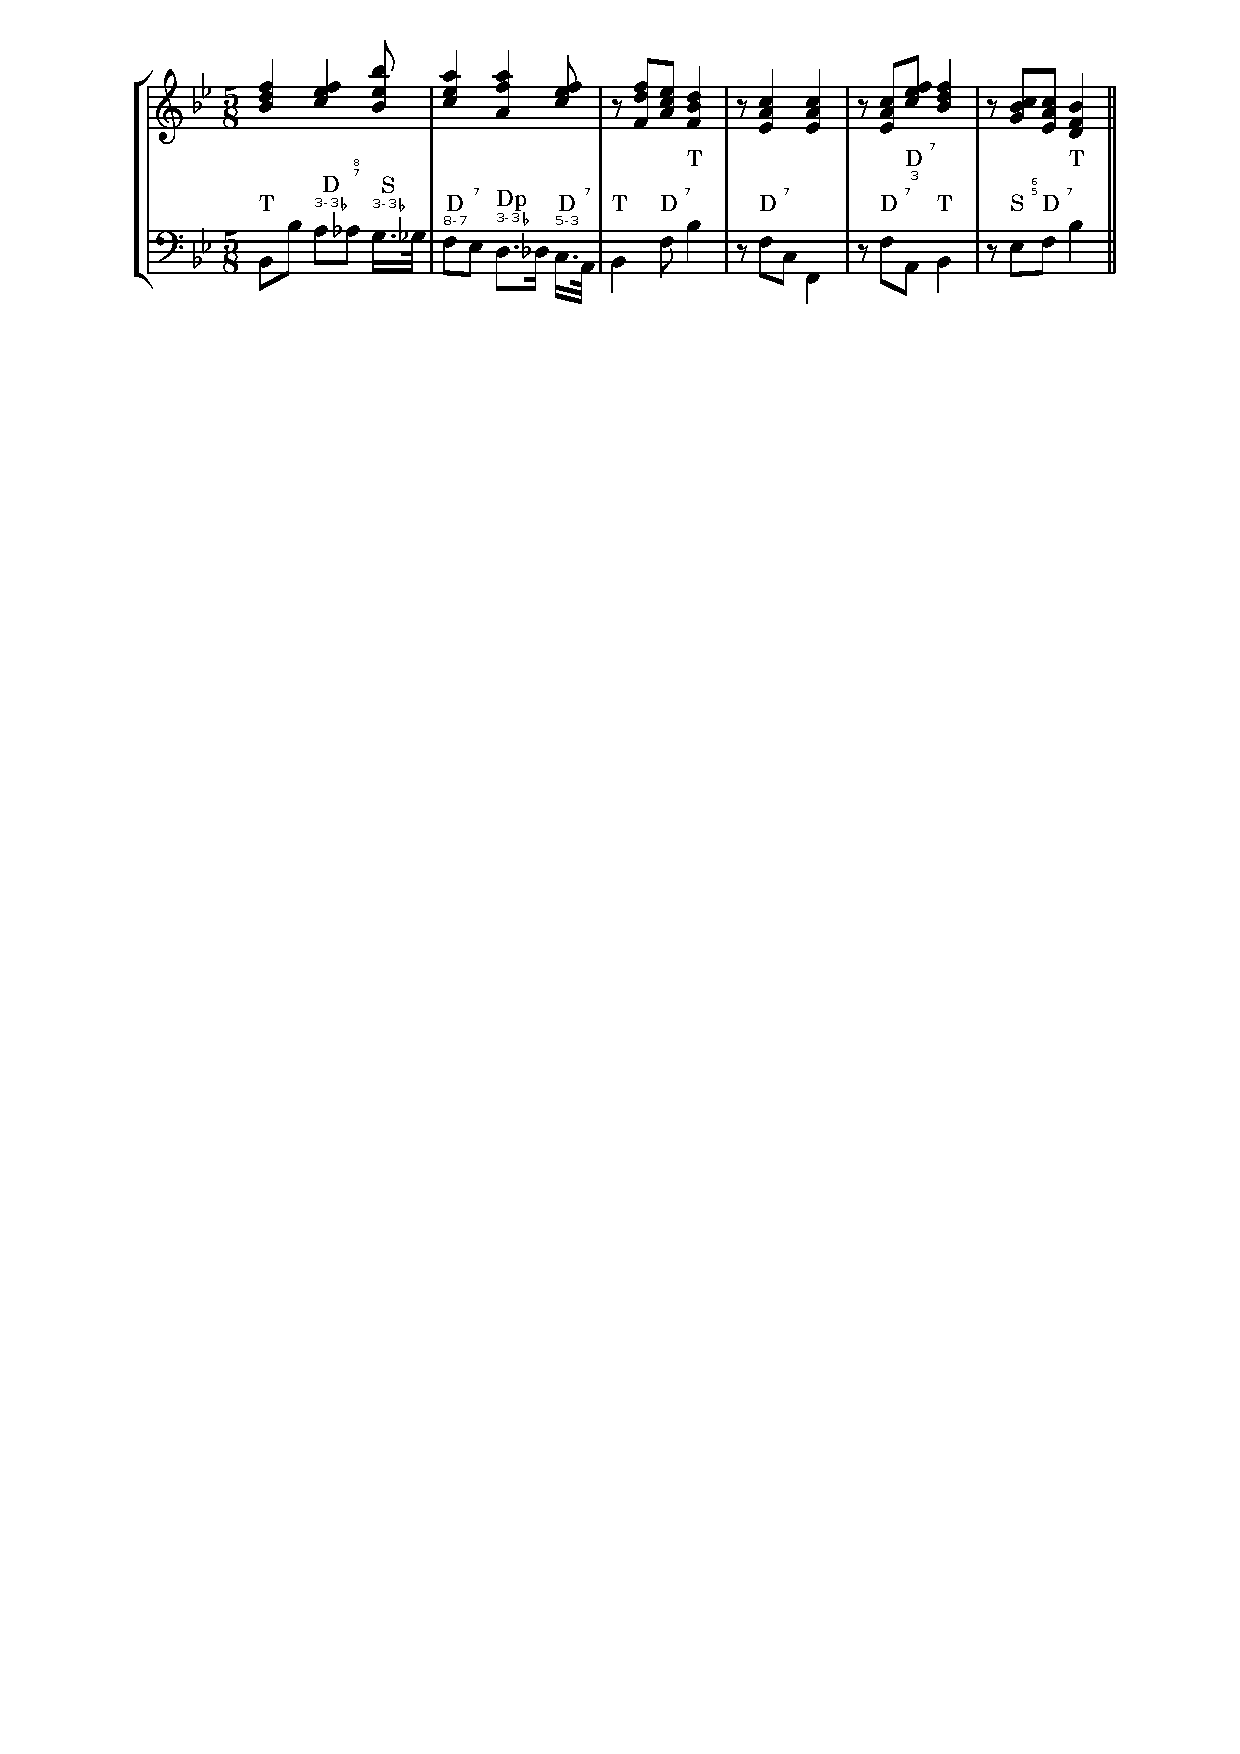
\includegraphics{pics/pmx/cadenca3}
\cad{III}{PMX}
\end{center}

Zu ihr gehört dieser Sourcecode:

\begin{verbatim}
%%% PREAMBLE: %%%%%%%%%%%%%%%%%%%%%%%%%%%%%%%%%%%%%%%%%%%%%%%%%%%%%%%
% nstaves | ninstr | mtrnuml  | mtrdenl | mtrnump | mtrdenp | npickup
     2        2         5          8         5         8         0
%  nkeys  | npages | nsystems | musicsize | fracident
     -2        0         3          16          .1
Bass
Diskant
bt
./
%%% BODY: %%%%%%%%%%%%%%%%%%%%%%%%%%%%%%%%%%%%%%%%%%%%%%%%%%%%%%%%%%% 
%%% HEADER: %%%%%%%%%%%%%%%%%%%%%%%%%%%%%%%%%%%%%%%%%%%%%%%%%%%%%%%%% 
\\font\ref=cmr10\def\zt#1#2{\zcharnote{#1}{\ref#2}}\def\bs{$\backslash$}\
%a smaller width than the line width
w130m
%%% MUSIC: %%%%%%%%%%%%%%%%%%%%%%%%%%%%%%%%%%%%%%%%%%%%%%%%%%%%%%%%%%%
%%% T1: %%%%%%%%%%%%%%%%%%%%%%%%%%%%%%%%%%%%%
[l b82 b8+ ] [l a8 a8f ] [l g1d g3 ] |/
\zt{-7}{T}\  b44u zd zf 
\zt{-7}{D7}\ cu ze zf 
\zt{-7}{S}\  b8-u ze zb+ |/
%%% T2: %%%%%%%%%%%%%%%%%%%%%%%%%%%%%%%%%%%%%
 [l f83 e83 ] [l d83d d13f ] [l c13d a32 ] |/
\zt{-7}{D7}\ c4-u ze za
\zt{-7}{Dp}\ a-u zd za+ 
\zt{-7}{D7}\ c8-u ze zf   |/
%%% T3: %%%%%%%%%%%%%%%%%%%%%%%%%%%%%%%%%%%%%
b42 f83 b43 |/
r8 \zt{-7}{T}\  [uh f85 zd zf-
   \zt{-7}{D7}\ e85 zc za ] 
   \zt{-7}{T}\  d4- zf zb |/
%%% T4: %%%%%%%%%%%%%%%%%%%%%%%%%%%%%%%%%%%%%
r8 f83 c83 f42 |/
r8 \zt{-7}{D7}\ e44 za zc e44 za zc |/
%%% T5: %%%%%%%%%%%%%%%%%%%%%%%%%%%%%%%%%%%%%
r8 [l f83 a8- ] b42l |/
r8 \zt{-7}{D7}\ [u c85 za ze c85 ze zf ] 
   \zt{-7}{T}\   b44u zf+ zd |/
%%% T6: %%%%%%%%%%%%%%%%%%%%%%%%%%%%%%%%%%%%%%
r8 [l e83 f8 ] b4l |/
r8 \zt{-7}{D7}\ [u c85 zb zg c85 za ze ] 
   \zt{-7}{T}\ b44u zf zd |/
%%%%%%%%%%%%%%%%%%%%%%%%%%%%%%%%%%%%%%%%%%% EOF
\end{verbatim}

Schon der erste Akkord aus der Musix\TeX-Variante
\begin{center}\texttt{\textbackslash{NOtes}
\textbackslash{Dqbl} I b \&
\textbackslash{zq}\{ik\}\textbackslash{qu}\{m\} \textbackslash{en}} \end{center}
reduziert\footnote{Um mal die reinen Notensymbole gegenüberzustellen, haben wir
diesmal die in beiden Varianten als \TeX-Code integrierten Analysesymbole n
weggelassen.} sich zum schlichteren
\begin{center}\texttt{[l b82 b8+ ] |/ b44u zd zf }\end{center}

\subsubsection{\ldots der Wermutstropfen \ldots}

Trotz der so euphorisch kolportierten Vorteile wächst sich \textit{PMX} bei
näherem Hinsehen für den Musikwissenschaftler jedoch zu einer Enttäuschung aus.
Gehen wir die Punkte der Reihe nach durch:

\paragraph{\small Inkompatibilitäten}$\;$ \\

Zunächst müssen wir 'gestehen', dass wir in diesem Kapitel unseres
'selbstreferentiellen' Dokumentes die Gegenüberstellung von Notentext und
generierendem Code nur scheinbar verwirklicht haben: Es gibt überhaupt keine
Möglichkeit, PMX-Code in \LaTeX-Code einzubetten und daraus dann -- sozusagen in
einem Rutsch -- eine PDF-Datei zu erzeugen.
Das liegt in erster Linie an der Arbeitsweise von \textit{PMX}\footnote{In zweiter
Linie liegt es an den Entwicklern von \textit{PMX}. Sie haben schlicht (noch) kein
korrespondierendes \LaTeX-Paket geschaffen. Technisch mag das herausfordernd
sein, unmöglich ist es nicht: Es wird ja schon gesagt, dass der von \textit{pmxab}
erzeugte Code eigentlich 'nur' auf die richtige Weise auskommentiert werden
müsse, damit er in der \texttt{\textbackslash{begin/end}\{music\}}-Umgebung
genutzt werden könne (\cite[vgl.][94]{Noack2013a}). Mithin sollte der Schritt zu
einer integrierten Lösung so groß nicht sein.}: Als Päprozessor nimmt das
entsprechende Tool \textit{pmxab} eine \textit{PMX}-Datei und erzeugt daraus eine
MusiX\TeX-Datei. Diese MusiX\TeX-Datei ist von ihrem Dialekt her aber eine
vollständige MusiX\TeX-Datei und kein inkludierbares Code-Snippet, das 1:1 in die
\LaTeX-Umgebung
\texttt{\textbackslash{begin}\{music\} \ldots \textbackslash{end}\{music\}}
eingebettet werden könnte. Entsprechende Versuche müssen scheitern.


\begin{verbbox}[\footnotesize]
.pmx.eps:
  @ make \$< `basename \$< .pmx`.tex
  @ musixtex -g `basename \$< .pmx`.tex
  @ ps2eps `basename \$< .pmx`.ps
.pmx.tex:
   @ pmxab \$<
\end{verbbox}

\label{PmxGraphics} Die eine, 'direkte' Lösung für dieses Problem besteht darin,
zuerst -- ganz \LaTeX-unabhängig -- aus der \textit{PMX}-Datei eine Graphik zu
erzeugen und diese anschließend in die \LaTeX-Datei einzubinden\footcite[Vgl.
dazu auch][94]{Noack2013a}:

\begin{itemize}
  \item Dazu ruft man für eine \textit{PMX}-Datei zunächst den
  \textit{PMX}-Präprozessor auf (z.B. \texttt{pmxab candeza1.pmx}), um die
  korrespondierende MusiX\TeX-Datei \texttt{candeza1.tex} zu genieren.
  \item Das Resultat übergibt man dann dem \textit{MusiX\TeX}-Tool als Input, und
  zwar mit der Option \textit{-g}: (\texttt{musixtex -g candeza1.tex}). So wird
  nicht eine \textit{PDF}-Datei erzeugt, sondern die Postscriptdatei
  \texttt{candeza1.ps}.
  \item Danach lässt man diese Postscriptdatei in eine 
  Encapsulated-Postscript-Datei umwandeln (\texttt{ps2eps
  candeza1.ps})\footnote{Eine make-basierte
  Automatisierung dieser Schritte enthielte als Kern wohl dies:\vspace{0.2em}\\
  \theverbbox\ \vspace{0.2em}\\
  \cite[Vgl. dazu][\nopage Makefile aus dem Verzeichnis 'pmx']{Reincke2019a}.}
  \item Und ganz zuletzt fügt man an der Stelle der \LaTeX-Datei, wo die
  \textit{eps}-Graphik erscheinen soll, den \LaTeX-Befehl 
  \texttt{\textbackslash{includegraphics}\{candeza1.eps\}}
  ein\footnote{Hier muss man beachten, an der Stelle, von wo aus man die
  \textit{eps}-Datei einlesen will, nicht (versehentlich) auch eine 'gleichnamige'
  \textit{pdf}-Datei abgelegt zu haben. In diesem Fall lädt
  \texttt{includegraphix} nämlich letztere. Und das wird im \LaTeX-Dokument zu
  unerwarteten Seitenumbrüchen führen, nach deren Ursache man u.U. lange sucht.
  }.
\end{itemize}

Diese Umstände müssen -- wenigstens den Musikwissenschaftler -- enttäuschen:
Wenn man zuletzt doch eine Graphik einbindet, die man mit einem externen Tool
erstellt hat, warum sollte man sich dann die Mühe antun, zwecks Erstellung einer
Graphik zuerst \textit{PMX} zu lernen, wo es doch so viele gute Notenprogramme
gibt, die ihre Daten auch als Postscript- oder PDF-Datei
exportieren?\footnote{Zu Erinnerung: \textit{ABC} geht implizit genauso vor.
Insofern träfe dieses Argument eben auch \textit{ABC}. Allerdings punktet
\textit{ABC} durch seine vielen Konverter und Tools und durch seine lange
Tradition.} Das könnte doch nur dann sinnvoll sein, wenn man wenigstens auf die
gestalterischen Vorzüge und Freiheiten von MusiX\TeX\ zugreifen könnte. Aber
nicht einmal das ist ja der Fall -- wie wir gleich sehen werden.

Zunächst müssen wir aber der Wahrheit Genüge tun und darauf hinweisen, dass der
Autor des \textit{PMX}-Tutorials sehr wohl um die Irritationen in Sachen \textit{PMX
/ MusiX\TeX}\ und \textit{\LaTeX}\ weiß, ja mehr noch, dass er sie auch nicht
verschweigt: Beide Ansätze würden  -- obwohl sie auf \TeX\ beruhen --
konkurrierend und überschneidend das Layout gestalten und viel Spezialbefehle
zueinander inkompatibel definieren\footcite[vgl.][93]{Noack2013a}. Und so kommt
er zu dem Schluss:

\begin{quote}\textit{\enquote{While with modern implementations of ressources
are no longer a serious problem, the incompatibility problems are, and their
resolution would be a major programming task. So there have, to this day, not
been any serious efforts to provide a truly merged version of \LaTeX\ with
PMX.}\footnote{\cite[vgl.][93f]{Noack2013a}. Man muss an dieser Stelle auch
im Kopf behalten, dass PMX nicht für die Nutzung in \LaTeX\ entwickelt worden ist.
Es ging den Entwicklern darum, besser und einfacher qualitativ hochwertige
Notenblätter zu erzeugen. Und für diesen Zweck ist die Lösung \textit{PMX
/ MusiX\TeX} sehr wohl geeignet. Nur ist die Gestaltung solcher Blätter meist nicht
Aufgabe von Musikwissenschaftlern.}
}\end{quote}

\paragraph{\small Unzulänglichkeiten}$\;$ \\

Die erste kleinere Unzulänglichkeit betrifft das Erscheinungsbild: Die
Kadenz-III in der \textit{PMX}-Variante\footnote{$\rightarrow$ S.
\pageref{\cadlab{III}{PMX}}} wirkt optisch weniger klar als die
\textit{MusiX\TeX}-Variante\footnote{$\rightarrow$ S.
\pageref{\cadlab{III}{MusiXTeX}}}. Dies liegt am 5/8-Takt. Der kann in eine 3er-
und eine 2er Hälfte oder in eine 2er und eine 3er Hälfte aufgeteilt werden. Und
das 3. Achtel der 3er-Hälfte kann auftaktisch gemeint sein. Die Entscheidungen,
die \textit{PMX} -- sozusagen nach Schema F -- automatisch trifft, können solchen
fallweisen Feinheiten natürlich nicht gerecht werden\footnote{Gelegentlich wird
man diese allerdings auch für reine Geschmacksfragen halten dürfen.}.

Die zweite Unzulänglichkeit betrifft die Methode, wie die Analysesymbole in den
\textit{PMX}-Code eingettet werden: \textit{PMX} bietet zwar die Möglichkeit, Stücke
auf \textit{PMX}-Level textuell zu kennzeichnen oder Texte über oder unter den
Systemen einzufügen\footcite[vgl.][61f]{Noack2013a}. Wenn es aber -- wie bei der
Musikwissenschaft notwendig -- darum geht, Symbole und Texte graphisch variabel
einzufügen, dann muss der \textit{PMX}-User auf \enquote{Inline \TeX\ commands}
zurückgreifen, also unter den \LaTeX-Level auf den \TeX-Level
'zurückfallen'\footcite[vgl.][76f]{Noack2013a}: die Nutzung einer vereinfachten
\textit{PMX}-Syntax wird dann um den Preis einer komplizierten Eingabe von
\TeX-Syntagmen erkauft\footnote{Weil \TeX\ 'zu' kompliziert war, wurde \LaTeX\
'erfunden'; und weil \textit{PMX} mit Text 'zu' kompliziert war, entstand
\textit{M-Tx} (\cite[vgl.][\nopage wp]{CtanMtx2018a}) -- einschließlich eines
Handbuches (\cite[vgl.][3ff]{Laurie2017a})}.

Wirklich unzulänglich ist dabei jedoch das, \textit{was} eingebettet werden kann.
Was schon bei den ABC-Lösungen galt\footnote{$\rightarrow$ S.
\pageref{AppraisalABC}}, gilt auch hier: Aus der \LaTeX-Welt können weder hoch-
und/oder tiefgestellte Kleinsymbole oder Sonderzeichen eingefügt werden, noch
die Alterationszeichen $\sharp$, $\flat$ oder $\natural$ aus den Sonderzeichen -
ganz zu schweigen von der Einbettung jener ausgefeilten Konstrukte, die das
\textit{harmony}-Paket zur Verfügung stellt. Denn das Konvertierungstool
\textit{pmxab}, das \textit{MusiX\TeX}-Code aus \textit{PMX}-Code ableitet, arbeitet
ja noch außerhalb von \TeX. Und das Konvertierungsttool \textit{musixtex}
versteht 'nur' \textit{Musix\TeX}-Code, nicht aber \LaTeX-Syntagmen.

\subsubsection{\ldots und die kleine Lösung: Kadenz II}

Trotz all dieser Nicklichkeiten kann es für den Musikwissenschaftler
gelegentlich sehr wohl Sinn machen, im Kontext einer \LaTeX-Arbeit\footnote{mit
inkludiertem MusiX\TeX-Package} auf \textit{PMX} zurückzugreifen: Wenn es nämlich
gilt, viele längere Musikbeispiele zu verwenden, wird das manuelle Tippen des
MusiX\TeX-Codes zu einer langwierigen, fehlerträchtigen Angelegenheit werden.

Eine Lösung dafür bestünde darin, zuerst den reinen Notentext mit \textit{PMX} zu
erstellen und dann mit \textit{pmxab} in MusiX\TeX-Code umzuwandeln. Danach griffe
man auf die Option zurück, -- wie im Tutorial als Möglichkeit angedeutet --
\enquote{manuell} bestimmte Zeilen des automatisch generierten Codes
auszukommentieren und so etwas zu erzeugen, was tatsächlich in die
\verb|\begin{music}...\end{music}|-\LaTeX-Umgebung kopiert werden
kann\footcite[vgl.][94]{Noack2013a}. Dieses Verfahren wollen wir noch kurz
vorführen:

Wir wissen ja schon, dass wir die Symbole der Harmonieanalyse, die wir auf
\textit{PMX}-Level erstellen könnten, bei einer Einbettung in einen \LaTeX-Code
werden nicht verwenden können, eben weil es ja keine \LaTeX-Konstrukte sind,
sondern \TeX-Syntagmen. Deshalb notieren wir diesmal auf \textit{PMX}-Level nur
den Notentext. Das 'reine' PMX/MusiX\TeX-Verfahren\footnote{PMX-Code $\rightarrow$
\texttt{pmxab} $\rightarrow$ Musix\TeX-Code $\rightarrow$ \texttt{musictex -g} 
$\rightarrow$ PS-Code  $\rightarrow$ \texttt{ps2eps} $\rightarrow$ EPS-Graphik }
würde daraus die folgende Graphik erzeugen:

\begin{center}
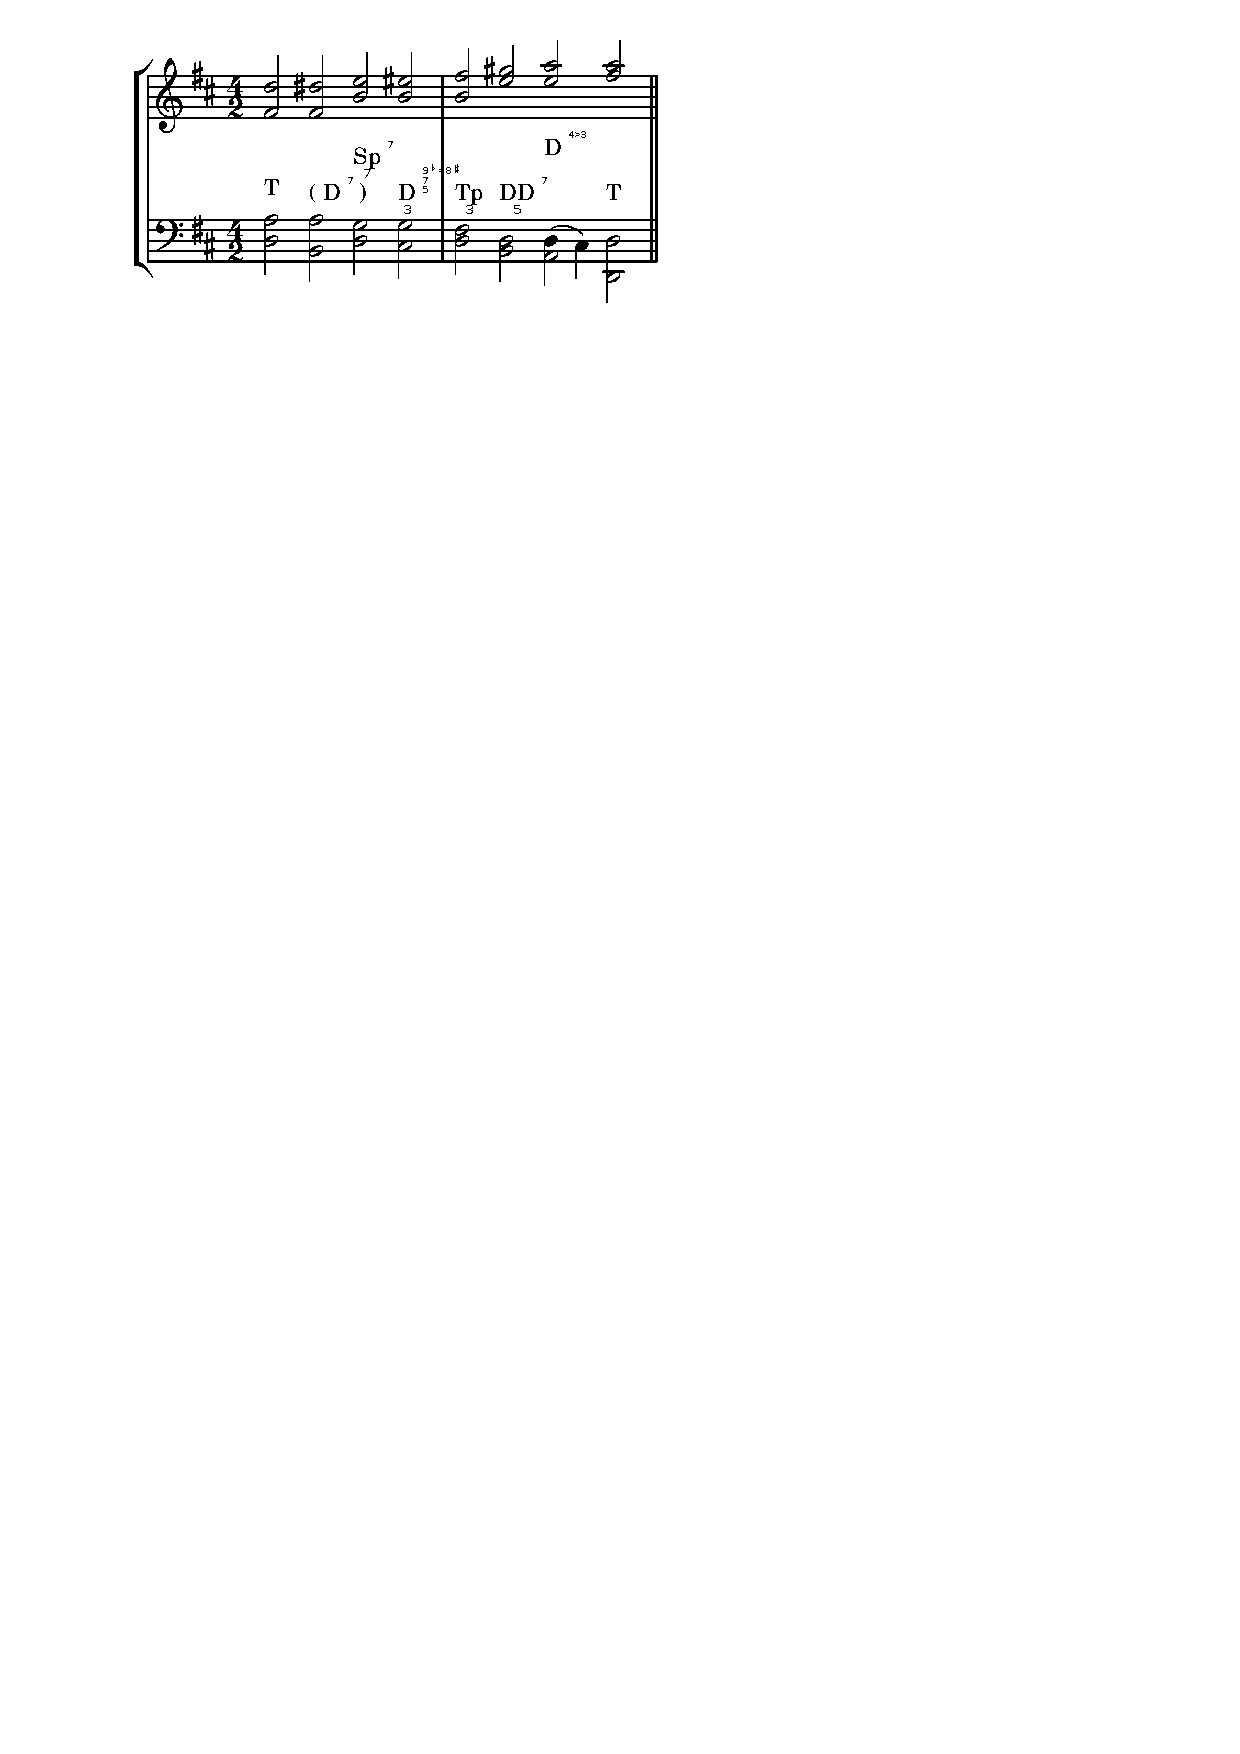
\includegraphics{pics/pmx/cadenca2}
\cad{II}{PMX}
\end{center}

Ausgegangen wird dabei von folgendem \textit{PMX}-Code:

\begin{verbatim}
% PREAMBLE %%%%%%%%%%%%%%%%%%%%%%%%%%%%%%%%%%%%%%%%%%%%%%%%%%%%%%%%%%
% nstaves | ninstr | mtrnuml  | mtrdenl | mtrnump | mtrdenp | npickup
     2        1         4          2         4         2         0
%  nkeys  | npages | nsystems | musicsize | fracident
     2        0         3          16          .1
Piano
bt
./
% BODY: %%%%%%%%%%%%%%%%%%%%%%%%%%%%%%%%%%%%%%%%%%%%%%%%%%%%%%%%%%%%%
% HEADER: %%%%%%%%%%%%%%%%%%%%%%%%%%%%%%%%%%%%%%%%
%a smaller width than the line width
w130m
% MUSIC: %%%%%%%%%%%%%%%%%%%%%%%%%%%%%%%%%%%%%%%%%
% T:1-1     T:1-2    T:1-3                T:1-4
  d23l za+  b-l za+  d-l zg              c-l zg+ |/
  f24u zd+  f-u zd+s  bu  ze              bu zes |/
% %%%%%%%%%%%%%%%%%%%%%%%%%%%%%%%%%%%%%%%%%%%%%%%%%
% T:2-1     T:2-2    T:2-3                T:2-4
  d23l zf  b-l  zd   (u d4 za2 c4 za2 )   d2-l zd+  /
  b24u zf+  e  zgs   e  za                f  za |/
% %%%%%%%%%%%%%%%%%%%%%%%%%%%%%%%%%%%%%%%%%%%%%  EOF 
\end{verbatim}

Lässt man diesen \textit{PMX}-Code von \texttt{pmxab} verarbeiten, entsteht ein
Musix\TeX-Code, bei dem man, will man ihn erfolgreich in eine
Musix\TeX-in-\LaTeX-Umgebung \verb|\begin{music}| ... \verb|\\end{music}|
einbetten, noch  einige Zeilen auskommentieren und einige Werte ändern muss:

\begin{verbatim}
\begin{music}
%%ignore:%% \input musixtex
%%ignore:%% \input pmx
%%ignore:%% \setmaxslurs{24}\setmaxinstruments{24}%
\normalmusicsize %%% instead of: %%% \smallmusicsize%
%%ignore:%% \nopagenumbers
%%ignore:%% \tracingstats=2\relax
%%ignore:%% \hsize=369pt
%%ignore:%% \vsize740pt
\def\nbinstruments{1}
\setstaffs12
\setclef1{60}
\setname1{Piano}
\generalsignature{ 2}%
\generalmeter{\meterfrac{4}{2}}%
\parindent 4em %%% instead of %%% 37pt
%%ignore:%% \elemskip1pt\afterruleskip1.000pt\beforeruleskip0pt\relax
%%ignore:%% \stafftopmarg0pt\staffbotmarg5\Interligne\interstaff{10}\relax
%%ignore:%% \readmod{cadenca2}
%%ignore:%% \startmuflex
\startpiece
%%ignore:%% \addspace
%%ignore:%% \afterruleskip%
%%ignore:%% \znotes|\zcharnote{16}{\titles{2.0}{}{0}{}{0}{}{0}}\en%
% Bar count 1
\pnotes{4.00}\zh{''A}\hl{`D}\zh{'A}\hl{`B}\zh G\hl D\zh G\hl C|\zh{'d}%
\hu{`f}\bigsh{'d}\zh d\hu{`f}\zh{'e}\hu b\bigsh e\zh e\hu b\en%
% Bar count 2
\xbar
\pnotes{4.00}\zh{'F}\hl D\zh D\hl B|\zh{'f}\hu b\bigsh g\zh g\hl e\en%
\pnotes{2.83}\zq A\qu D \zq A\qu C|\zh{''a}\hl{`e}%
%%ignore: \isu0{'D}{.8} \tslur0A
\en%
\pnotes{4.00}\zh{'D}\hl{`D}|\zh{''a}\hl{`f}\en%
\Endpiece
%%ignore:%% \vfill\eject\endmuflex
%%ignore:%% \bye
\end{music}%
\end{verbatim}

Vor einer erfolgreichen Nutzung diese Codes muss man in seinem \LaTeX-Header
auch noch die Regel \verb|\newcommand{\pnotes}[1]{\notes}| formuliert haben,
damit aus der Einbettung auf \LaTeX/MusiX\TeX-Ebene -- also ohne Einbindung
einer externen Graphik -- das folgende Bild  entsteht:

\vspace{0.7cm}
\begin{music}
%%ignore:%% \input musixtex
%%ignore:%% \input pmx
%%ignore:%% \setmaxslurs{24}\setmaxinstruments{24}%
\normalmusicsize %%% instead of: %%% \smallmusicsize%
%%ignore:%% \nopagenumbers
%%ignore:%% \tracingstats=2\relax
%%ignore:%% \hsize=369pt
%%ignore:%% \vsize740pt
\def\nbinstruments{1}
\setstaffs12
\setclef1{60}
\setname1{Piano}
\generalsignature{ 2}%
\generalmeter{\meterfrac{4}{2}}%
\parindent 4em %%% instead of %%% 37pt
%%ignore:%% \elemskip1pt\afterruleskip1.000pt\beforeruleskip0pt\relax
%%ignore:%% \stafftopmarg0pt\staffbotmarg5\Interligne\interstaff{10}\relax
%%ignore:%% \readmod{cadenca2}
%%ignore:%% \startmuflex
\startpiece
%%ignore:%% \addspace
%%ignore:%% \afterruleskip%
%%ignore:%% \znotes|\zcharnote{16}{\titles{2.0}{}{0}{}{0}{}{0}}\en%
% Bar count 1
\pnotes{4.00}\zh{''A}\hl{`D}\zh{'A}\hl{`B}\zh G\hl D\zh G\hl C|\zh{'d}%
\hu{`f}\bigsh{'d}\zh d\hu{`f}\zh{'e}\hu b\bigsh e\zh e\hu b\en%
% Bar count 2
\xbar
\pnotes{4.00}\zh{'F}\hl D\zh D\hl B|\zh{'f}\hu b\bigsh g\zh g\hl e\en%
\pnotes{2.83}\zq A\qu D \zq A\qu C|\zh{''a}\hl{`e}%
%%ignore: \isu0{'D}{.8} \tslur0A
\en%
\pnotes{4.00}\zh{'D}\hl{`D}|\zh{''a}\hl{`f}\en%
\Endpiece
%%ignore:%% \vfill\eject\endmuflex
%%ignore:%% \bye
\end{music}%
\cad{II}{PMX+MusiXTeX-in-LaTeX}
\vspace{0.7cm}

An dieser Version erkennt man jedoch auch, dass die Vorstellung, man brauche
bloß mal eben Zeilen auszukommentieren, der Sachlage nicht gerecht wird: Damit
obiger Code überhaupt kompilierbar wurde, mussten wir die Vorhaltsklammer im
Bass aus dem Code herausnehmen, was dort unmittelbar zu einer ungewollten
Oktavierung führte. Tatsächlich wird man -- falls man den MusiX\TeX-Code in
seinen \LaTeX-Code einfügen will, den \texttt{pmxab} aus der \textit{pmx}-Datei
erzeugt -- ein wenig 'Tuning'-Zeit einplanen müssen. Geht man diesen Weg, kann
man nun allerdings auch die \LaTeX-basierten Elemente einer Harmonieanalyse
darin verwenden. Man hat also in der Tat die gestalterische Freiheit auf
\LaTeX-MusiX\TeX-Level gewonnen, ohne den komplexen und komplizierten
MusiX\TeX-Code als Ganzes selbst entworfen haben zu müssen. Die Grundarbeit
erledigt man auf \textit{PMX}-Level, die Feinheiten fügt man manuell ein:

\vspace{0.7cm}
\begin{music}%
\normalmusicsize %%% instead of: %%% \smallmusicsize%
\def\nbinstruments{1}
\setstaffs12
\setclef1{60}
\setname1{Piano}
\generalsignature{ 2}%
\generalmeter{\meterfrac{4}{2}}%
\parindent 4em %%% instead of %%% 37pt
\startpiece
% Bar count 1
\notes
  \zmidstaff{\HH.T.....}\zh{''A}\hl{`D}%
  \zmidstaff{(\HH.D..7...)}\zh{'A}\hl{`B}%
  \zmidstaff{\HH.Sp.7...7.}\zh G\hl D
  \zmidstaff{\HH.\Dohne.3.$\flat$9=$\sharp$8.7.5.}\zh G\hl C |%
  \zh{'d}\hu{`f}\bigsh{'d}\zh d\hu{`f}%
  \zh{'e}\hu b\bigsh{e}\zh e\hu b%
\en%
% Bar count 2
\xbar
\notes
  \zmidstaff{\HH.Tp.3....}\zh{'F}\hl D%
  \zmidstaff{\HH.\DD.5...7.}\zh D\hl B |%
  \zh{'f}\hu b\bigsh g%
  \zh g\hl e%
\en%
\notes
  \zmidstaff{\HH.D....4-3.}%
  \zh{H}\isluru{0}{K}\qu{K}\tslur{0}{J}\qu{J}|%
  \zh{''a}\hl{`e}%
\en%
\notes
  \zmidstaff{\HH.T.....}\zh{'D}\hl{`D}  |%
  \zh{''a}\hl{`f}%
\en%
\Endpiece
\end{music}%
\cad{II}{PMX+MusiXTeX-in-LaTeX++}
\vspace{0.7cm}
 
Hilfreich sind dabei -- zugegebenermaßen -- Geduld, ein geschulter Blick und der
Wille zum Codeclearing:

\begin{verbatim}
\begin{music}%
\normalmusicsize %%% instead of: %%% \smallmusicsize%
\def\nbinstruments{1}
\setstaffs12
\setclef1{60}
\setname1{Piano}
\generalsignature{ 2}%
\generalmeter{\meterfrac{4}{2}}%
\parindent 4em %%% instead of %%% 37pt
\startpiece
% Bar count 1
\notes
  \zmidstaff{\HH.T.....}\zh{''A}\hl{`D}%
  \zmidstaff{(\HH.D..7...)}\zh{'A}\hl{`B}%
  \zmidstaff{\HH.Sp.7...7.}\zh G\hl D
  \zmidstaff{\HH.\Dohne.3.$\flat$9=$\sharp$8.7.5.}\zh G\hl C |%
  \zh{'d}\hu{`f}\bigsh{'d}\zh d\hu{`f}%
  \zh{'e}\hu b\bigsh{e}\zh e\hu b%
\en%
% Bar count 2
\xbar
\notes
  \zmidstaff{\HH.Tp.3....}\zh{'F}\hl D%
  \zmidstaff{\HH.\DD.5...7.}\zh D\hl B |%
  \zh{'f}\hu b\bigsh g%
  \zh g\hl e%
\en%
\notes
  \zmidstaff{\HH.D....4-3.}%
  \zh{H}\isluru{0}{K}\qu{K}\tslur{0}{J}\qu{J}|%
  \zh{''a}\hl{`e}%
\en%
\notes
  \zmidstaff{\HH.T.....}\zh{'D}\hl{`D}  |%
  \zh{''a}\hl{`f}%
\en%
\Endpiece
\end{music}
\end{verbatim}


% this is only inserted to eject fault messages in texlipse
% \bibliography{../bib/literature}


% mycsrf 'for beeing included' snippet template
%
% (c) Karsten Reincke, Frankfurt a.M. 2012, ff.
%
% This text is licensed under the Creative Commons Attribution 3.0 Germany
% License (http://creativecommons.org/licenses/by/3.0/de/): Feel free to share
% (to copy, distribute and transmit) or to remix (to adapt) it, if you respect
% how you must attribute the work in the manner specified by the author(s):
% \newline
% In an internet based reuse please link the reused parts to mycsrf.fodina.de
% and mention the original author Karsten Reincke in a suitable manner. In a
% paper-like reuse please insert a short hint to mycsrf.fodina.de and to the
% original author, Karsten Reincke, into your preface. For normal quotations
% please use the scientific standard to cite
%


%% use all entries of the bibliography

\subsection{Lilypond: so schön, wie vielversprechend ($\bigstar\bigstar\bigstar\bigstar\bigstar$)}

\parpic(2cm,1.4cm)[r][t]{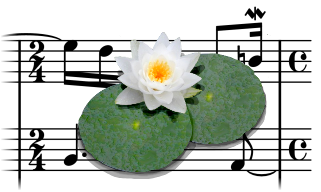
\includegraphics[width=2cm]{logos/lilypond-300dpi.png}}
\textit{LilyPond} möchte guten \enquote{Notensatz für jedermann} anbieten: Als
elektronisches \enquote{Notensatzsystem} -- so das Entwicklungsteam -- wolle es
\enquote{[\ldots] Notendruck in (bester) Qualität} ermöglichen, mithin
\enquote{[\ldots] die Ästhetik handgestochenen traditionellen Notensatzes mit
computergesetzten Noten [\ldots] erreichen}.\footnote{\cite[vgl.][\nopage
wp]{LilyPond2018a}. Lizensiert ist \acc{LiyPond} unter der GPL $\rightarrow$
\href{http://lilypond.org/gpl.html}{http://lilypond.org/gpl.html}, einer
anerkannten Open-Source-Lizenz ($\rightarrow$
\href{https://opensource.org/licenses/GPL-2.0}
{https://opensource.org/licenses/GPL-2.0}). } In einem besonderen Artikel haben
die LilyPond-Entwickler dargestellt, was das systemisch
bedeutet\footcite[vgl.][5ff]{LilyPond2018d} und welchen Konsequenzen sich daraus
für ein Notensatzprogramm ergeben.\footcite[vgl.][8ff]{LilyPond2018d} Der daraus
erwachsende Anspruch ist hoch:

\begin{quote}\textit{\enquote{LilyPond wurde geschaffen, um die Probleme zu
lösen, die wir in existierenden Programmen gefunden haben und um schöne Noten zu
schaffen, die die besten handgestochenen Partituren
imitieren.}\footcite[vgl.][2]{LilyPond2018d} }
\end{quote}

Wer die entsprechenden Techniken erfolgreich anwenden will, kann auf ein einfach
strukturiertes Lerntutorial\footcite[vgl.][20ff]{LilyPond2018b} und ein kürzeres
Nutzungshandbuch\footcite[vgl.][1ff]{LilyPond2018e} zurückgreifen. Letztlich
wird er sich allerdings auch das umfangreiche
Notationshandbuch\footcite[vgl.][1ff]{LilyPond2018c} bereitlegen wollen.

Wie die bisher diskutierten Systeme erwartet \textit{LilyPond}, dass man Code
schreibt, keine Noten: Hier wie da ist der Texteditor das bevorzugte Werkzeug,
um Musik im entsprechenden 'Dialekt' zu notieren. Trotzdem gibt es Unterschiede,
die über die bloße Syntax hinausgehen:

Die wichtigste Eigenart dürfte sein, dass Lilypond konsequent zwischen Musik und
Druck unterscheidet: Wer in D-Dur ein \textit{fis} einfügen möchte, kann sich
hier nicht auf die zu Beginn spezifizierte Tonart 'berufen', er muss trotzdem
\texttt{fis} tippen, nicht \texttt{f}, und zwar an jeder Stelle, wo er
\textit{fis} meint. Diese Abkehr von der musikalischen Tradition hat einen
gewichtigen Vorteil: Lilypond kann bei Alterationen die nötigen Vorzeichen
automatisch setzen. In \textit{g-moll} erhält die Note \textit{f} bei
eingegebenem \texttt{fis} automatisch ein Kreuz, in D-Dur
nicht.\footnote{\cite[vgl.][21]{LilyPond2018b}. In der Konsequenz wird man sich
allerdings auch an -- wenigstens für Deutsche -- überraschende 'Töne' wie
\texttt{bes}, \texttt{beses} oder \texttt{bis} gewöhnen müssen.}

Die augenfälligste Besonderheit dürfte jedoch sein, dass \textit{LilyPond} seine
Elemente konsequent in einer 1:n-Beziehung anordnet: Das Notenheft besteht aus
einem oder mehreren Stücken, das Stück besteht aus einem oder mehreren
Notensystemen, ein Notensystem besteht aus einer oder mehrerer Stimmen, die
Stimme kann solistisch oder akkordisch sein. Das Datenmodell ist mithin als
Baum\footcite[vgl.][\nopage wp.]{WpedBaum2019a} ausgelegt. Und syntaktisch haben
die Ebenen je eigene Markanten. Das macht das Lesen und Verstehen von
\textit{LilyPond}-Code auf Dauer einfacher, es entsteht ein klarerer
Sourcetext.\footcite[vgl.][40ff]{LilyPond2018b}

Systemisch gesehen hat LilyPond (heute) nichts (mehr) \LaTeX\ , MusiX\TeX\ oder
\TeX\ zu tun: es nutzt seine eigene Eingabesprache und seine eigene Maschine zum
Erzeugen des Notenbildes: Als \enquote{Standardausgabeformat} -- heißt es --
seien \textit{PDF}\footnote{Portable Document Format} und
\textit{PS}\footnote{Postscript} gesetzt; außerdem könnten
\textit{SVG\footnote{Scalable Vector Graphics}-}, \textit{EPS\footnote{Encapsulated
PostScript}-} und \textit{PNG\footnote{Portable Network Graphics}-}Dateien erzeugt
werden.\footcite[vgl.][481]{LilyPond2018c}

\subsubsection{Technische Voraussetzungen}

\textit{LilyPond} sagt selbst, dass man Notenbeispiele in Form von Graphiken auch
manuell in den \LaTeX-Text einfügen könne, einfach indem man -- zuerst und
unabhängig von \LaTeX\ -- die Graphiken mit \texttt{lilypond} erzeuge und sie
danach mit \LaTeX-Mitteln einbinde.\footcite[vgl.][20]{LilyPond2018e} Bei vielen
Notenbeispielen kann das allerdings aufwendig werden, insbesondere, wenn man
manuell die Länge der Notenzeilen und die Graphikbreite auf die gewünschte
Zeilenlänge des Dokumentes ausrichten muss.

Deshalb bietet \textit{LilyPond} nicht nur das Tool \texttt{lilypond} zur
Erzeugung ganzer Notenblätter in den genannten Formaten an\footnote{samt aller
anderen Outputformate wie \textit{midi} u.Ä.m.}, sondern auch das Tool
\texttt{lilypond-book}: dieses \enquote{automatisiert} die manuelle Integration,
indem es die \enquote{[\ldots] Musik-Schnipsel aus Ihrem Dokument (extrahiert),
[\ldots] \texttt{lilypond} (aufruft) und [\ldots] die resultierenden Bilder in
Ihr Dokument (einfügt)}, wobei es \enquote{[\ldots] die Länge der Zeilen und die
Schriftgröße dabei [automatisch] (dem) Dokument
(anpasst)}.\footcite[vgl.][20]{LilyPond2018e}

Daraus folgt sofort, dass man auch hier einiges vorzubereiten hat, wenn man
\textit{LilyPond} erfolgreich verwenden will:

$\RHD$ Zunächst muss man -- ganz unabhängig von \LaTeX\ -- \textit{LilyPond}
installieren\footnote{Unter Ubuntu: \texttt{sudo apt-get lilypond
lilypond-data}}. Dieses Paket stellt dann auch \texttt{lilypond-book} bereit.
  
$\RHD$ Im Gegensatz zu \textit{ABC} oder \textit{MusiX\TeX} braucht \acc{LilyPond}
nicht in der \LaTeX-Präambel aktiviert zu werden. Denn \texttt{lilypond-book} muss
ja immer zuerst und unabhängig von \LaTeX\ aufgerufen werden: Es generiert erst den
eigentlichen \LaTeX-Code, der dann keine \textit{LilyPond}-Sektionen mehr
enthält. Also kann man -- direkt nach der Installation -- den
\textit{LilyPond}-Quelltext eines jeden Notenbeispiels in je einer eigenen
(virtuellen) Umgebung \verb|\begin{lilypond}...\end{lilypond}| editieren.
Virtuell sind diese Umgebungen insofern, als \LaTeX\ ja nichts von
\textit{LilyPond} weiß.

$\RHD$ Schließlich muss man noch organisieren, dass den eigentlichen
\LaTeX-Durchgängen zur Generierung der PDFs ein \texttt{lilypond-book}-Aufruf
vorausgeht. Das kann wieder in einem Makefile organisiert werden.

Leider steckt der Teufel dabei -- wie so oft -- im Detail: 

\label{LilyPondGraphics}\texttt{lilypond-book} nimmt eine -- wie wir jetzt
wissen -- gewissermaßen 'unechte' \LaTeX-Datei, die noch
\textit{lilypond}-Sektionen enthält, und erzeugt die entsprechenden Graphiken,
bevor es die \textit{lilypond}-Sektionen durch die korrespondierenden
'include-Graphik'-Befehle auf \LaTeX-Ebene ersetzt. Das ist der Grund, warum
\texttt{lilypond-book} immer als erstes prozessiert werden muss.

Ruft man \texttt{lilypond-book} ohne weitere Parameter für eine ('unechte')
\LaTeX-Datei mit der Extension \textit{.tex} auf, beschwert es sich, dass es seine
Inputdatei überschreiben müsste und verweigert die Weiterarbeit. Dies wird
gelöst, indem man es mit der Option \texttt{--out IHRDIR} aufruft. Dann erzeugt
\texttt{lilypond-book} einen Ordner names \textit{IHRDIR} und sammelt darin
alle Materialien ein, die es für eine \LaTeX-compilierbare Version benötigt.

Unglücklicherweise muss man \texttt{lilypond-book} dabei ein wenig unter die Arme
greifen:

Tatsächlich evaluiert und bearbeitet \texttt{lilypond-book} erfolgreich alle
Dateien mit der Extension \textit{.tex}, insbesondere auch die, die per
\textit{input}-Befehl in die Hauptdatei eingebunden worden sind. Die Aufteilung
eines LaTeX-Textes in mehrere 'Snippets' bedeutet für \texttt{lilypond-book} kein
Problem. Und \texttt{lilypond-book} kopiert auch alle gefundenen Daten -- ggfls.
überarbeitet -- korrekt in den Arbeitsordner, den man dem Tool auf der
Kommandozeile mit gegeben hat, und zwar unter Beibehaltung der Ordnerstrukturen,
sodass die include-Referenzen in den kopierten Dateien nicht ins Leere zeigen.
Gleichwohl gibt es Dateien, die nicht in den Blick von \texttt{lilypond-book}
geraten und die es darum auch nicht mit in den Arbeitsordner übernimmt. Trotzdem
werden natürlich auch diese Dateien benötigt, wenn man innerhalb des
Arbeitsordners erfolgreich einen \LaTeX-Lauf starten will. Prominentestes
Beispiel für solche Dateien sind die \textit{bib-Files} und ausgelagerte
Konfigurationsdateien.

Deshalb muss der \LaTeX-User als Nutzer von \texttt{lilypond-book} -- sozusagen
manuell -- die fehlenden Dateien in den von \texttt{lilypond-book} erzeugten
Arbeitsordner kopieren, bevor er den 'normalen' \LaTeX-Erzegungsprozess aufruft.

Eine entsprechendes Makefile könnte so aussehen:

\begin{verbatim}

# source directory
SRCD=source
# lilypond working directory
LPWD=lily

prod: 
  # (1) create a copy of your source directory as lilypond directory 
  @ cp -rd ${SRCD} ${LPWD}
  # (2) change into the lilypond directory and call lilypond for your
  #     file & let the results be written into a temporary directory
  @ ( cd ${LPWD} && lilypond-book --out ../tmp your-latex-file.tex )
  # (3) lilypond has created & collected the sources it needs into the 
  #     tmp dir but unfortunatelay not all. Hence, 
  #     the missed parts must still be copied into that tmp dir manually
  # (4.a) ensure that all dirs really exist we need
  @ mkdir -p  tmp/bib/ tmp/cfg tmp/pics
  # (4.b) ensure that also the missed files can be found in the tmp dir
  @ cp -rd ${SRCD}/bib/* tmp/bib/
  @ cp -rd ${SRCD}/cfg/* tmp/cfg/
  @ cp ${SRCD}/Makefile tmp/
  ( cd tmp && make your-latex-file.pdf && mv your-latex-file.pdf ../ )
  rm -rf ${LPWD}
  rm -rf tmp

\end{verbatim}


\subsubsection{Kadenz I}
\label{LilyPondKadenzI}
Und damit dürfen wir die Früchte der Vorarbeit ernten: Es ist bereits
absehbar, dass die eigentliche Herausforderung zuletzt nicht mehr die Nutzung
von \textit{LilyPond} als solches sein wird, sondern die Einbindung jener
Symbole in den Notentext, die für den Musikwissenschaftler so wichtig sind.
\textit{LilyPond} selbst bietet 3 Verfahren an, (echten) Text in die Noten zu
integrieren:

\begin{enumerate}
  \item Man darf 'Liedtext' unter ein Notensystem setzen, wobei als Text dort
  auch -- in einfacher Form  -- Analysesymbole erscheinen können.
  können.\footcite[vgl.][31ff]{LilyPond2018b}
  \item Man darf Makros mit Text an Noten anhängen, die dann -- je nach
  Vorzeichen '\texttt{\_}' oder '\texttt{\^}' über oder unter der Note
  erscheinen. Diese Makros gibt es in einer verkürzten und einer expliziten
  Version. Beide sind Sonderfälle einer generellen
  Markupsprache.\footcite[vgl.][211ff]{LilyPond2018c}
  \item Man darf komplexer strukturierte Syntagmen der erwähnten generalisierten
  Markupsprache an Noten anhängen, mit denen es dann auch möglich wird, feinere
  Texte differenziert zu gestalten und
  einzufügen.\footcite[vgl.][218ff]{LilyPond2018c} 
\end{enumerate}

Dabei wird der Musikwissenschaftler nicht auf die \LaTeX-Sonderzeichen oder die
schönen \textit{harmony}-Konstrukte zurückgreifen können. Denn \textit{LilyPond}
arbeitet ja \LaTeX-unabhängig. Also wird über die Brauchbarkeit von
\textit{LilyPond} letzlich die Frage entscheiden, ob und wie gut man die Symbole
der Harmonieanalyse, die \textit{harmony} bereitstellt, mit den Mitteln von
\textit{LilyPond} nachbilden kann und welcher Aufwand dabei entsteht.

Gehen wir diese Dinge der Reihe nach durch, beginnend -- wie kaum anders zu
erwarten -- mit der einzeiligen
Grabner-Kadenz\footcite[vgl.][107]{Grabner1974a}: Die ersten beiden Akkorde sind
mit einfachen Markups klassifiziert, der dritte mit der entsprechenden
abgekürzten Version. Und unter den letzten drei Akkorden sind die Symbole als
'Liedtext' eingefügt worden:

\begin{center}
\begin{lilypond}
\version "2.18.2"

\header { tagline = "" }
\score {
  \new Staff {
    \relative c' { 
      \time 3/1
      <c e g>1 _\markup {I} ^\markup {T}
      <f a c>  _\markup {IV} ^\markup {S}
      <g b d>  _"V" ^"D"
      |
      {	<< 
      	  {
            <a, c e>  ^"T"
            <d f a>   ^"S"
            <e gis b> ^"D"
          }
          \addlyrics {
          	I IV V
          }
        >>
      }
      \bar "||"
    }   
  }
  \layout {
    \context {
      \Staff
        \remove Time_signature_engraver
    }
  }
}
\end{lilypond}
\cad{I}{LilyPond}
\end{center}

Man sieht, dass die einfacheren Markup-Konstrukte noch auf einer Linie
ausgerichtet werden müssten. Das ist bei der Methode 'Liedtext' schon implizit --
im Rahmen der Implementation --  erledigt worden. Der zugehörige Quellcode sieht
so aus:
\begin{verbatim}
\begin{lilypond}
\version "2.18.2"
\header { tagline = "" }
\score {
  \new Staff {
    \relative c' { 
      \time 3/1
      <c e g>1 _\markup {I} ^\markup {T}
      <f a c>  _\markup {IV} ^\markup {S}
      <g b d>  _"V" ^"D"
      |
      { << 
          {
            <a, c e>  ^"T"
            <d f a>   ^"S"
            <e gis b> ^"D"
          }
          \addlyrics {
            I IV V
          }
        >>
      }
      \bar "||"
    }   
  }
  \layout {
    \context {
      \Staff
        \remove Time_signature_engraver
    }
  }
}
\end{lilypond}
\end{verbatim}

An diesem Code erkennt man gut die systematische 1:n-Struktur eines
\textit{LilyPond}-Quelltextes: Der \texttt{score} hat eine Stimme
(\texttt{staff}). All ihre Noten beziehen sich sich auf \texttt{c'}. Und sie hat
vier Abschnitte, nämlich drei Akkorde \texttt{< \ldots\ >}, gefolgt von einer
strukturierten Einheit. Dieser Komplex besteht seinerseits aus zwei Teilen, die
'gleichzeitig' (= übereinander) abgedruckt werden sollen: nochmals 3 Akkorde und
die 3 Symbole, die darunter erscheinen.

Es zeigt sich aber auch, dass die naheliegenden Methoden,
Funktionsanalysesymbole in die Noten zu integrieren, inhaltlich gesehen nicht
ausdrucksreich genug sind und optisch nicht zufrieden stellen. Hier wird man
etwas tun müssen. 

\subsubsection{Kadenz II}

\textit{LilyPond} ist nicht nur 'waschechte' \textit{Open-Source-Software}, sondern
kommt zudem mit einer Erweiterungssprache daher.\footcite[vgl. dazu][\nopage
wp]{WpedGuile2019a} Diese zu nutzen, um die Möglichkeiten vom \LaTeX-Paket
\textit{harmony} nachzubilden, artet jedoch in echte Programmierarbeit aus und
dürfte einem Musikwissenschaftler kaum mehr zuzumuten sein - wohl aber denen,
der in beiden Welten zuhause ist, also uns.

\label{LilyPondFuncTheory}Wir haben deshalb begonnen, eine kleine
\textit{LilyPond}-Library zu entwickeln, die man einfach in seine
\textit{LilyPond}-Datei mit dem Befehl \texttt{\textbackslash{include}}
hinzulädt. Danach kann man die entsprechende Symbole der Harmonieanalyse in
seinen Notentext hinzufügen. Unsere aktuelle stabile Version liefert folgendes
-- sicher noch nicht ganz optimales -- Ergebnis\footnote{Die Einschränkungen
werden aber nicht so bleiben! Z.Zt.
benötigen wir noch \ldots
\begin{itemize}
  \item die Möglichkeit, innerhalb des \textit{LilyPond}-Markups Zeichen
  übereinander zu schreiben, um Symbole für die Doppeldominante, die
  Doppelsubdominante und für das Fehlen von etwas ('Schräge Durchstreichung')
  generieren zu können. Ohne eine solche Kennzeichnung bleibt die
  Funktionsbezeichnung für den 4. Akkord ungenau, denn der Grundton ist ja nicht
  im Akkord enthalten.
  \item die Option, Noten und Markupblock horizontal auszurichten, sodass auch
  komplexe Analysesymbole über resp. unter genau den Akkordnoten stehen, auf die
  sie sich beziehen. Ohne eine solche Ausrichtung rutscht die Spezifikation des
  2. Akkordes aus der Reihe und die des 4. Akkordes ragt in den nächsten Takt
  hinein.
  \item die Möglichkeit, die hochgestellten Akkordzahlen näher an das
  Grundsymbol heranzurücken, um Zusammenhänge optisch zu verdeutlichen.
  \item die \textit{Guile-} resp. \textit{LilyPond}-Techniken zum Refactoring,
  sodass derselbe Code nicht mehrfach in der Bibliothek auftauchen muss, sondern
  einmal programmiert und ansonsten wiederverwendet wird.
\end{itemize}}:


\begin{center}
\begin{lilypond}
\version "2.18.2"

\header { tagline = "" }

\include "lilypond/inc.hanalysis.ly"
  
\score {
  \new StaffGroup {
    \time 4/2
    <<
      \new Staff {
        \relative d' {
          \clef "treble"
          \key d \major  
          \stemUp
         < fis  d'>2    
          < fis  dis'>2   
          < b  e>2        
          < b  eis>2        
          | 
          < b fis'>2  
          < e gis >2  
          < e a >2    
          < a fis>2      
          \bar "||"
        }   
      }
      \new Staff {
        \relative d { 
          \clef "bass"
          \key d \major  
          \stemDown
          < d a'>2        ^\markup { \hf T }                      
          < b a'>2        ^\markup { ( \hfOne D "7" ) }           
          < d g>2         ^\markup { \hfiOne Sp "7" "7" }         
          < cis g'>2      ^\markup { \hfiTri D "3" "5" "7" 
                                        \line{"9"{\super{\flat}}"=8"{\super{\sharp}}}
                                    }                               
          |
          < d fis>2       ^\markup { \hfi Tp "3" }                
          < b d>2         ^\markup { \hfiOne DD "5" "7" }         
          <<
            { a2          ^\markup { \hfOne D "4>3" }  }
            { d4( cis4) }
          >> 
          < d, d'>2       ^\markup { \hf T }
          \bar "||"
        }   
      }
    >>
  }
}
\end{lilypond}
\cad{II}{LilyPond}
\end{center}

Mit Rückgriff auf diese kleine Zusatzbibliothek sähe der entsprechende
\textit{Lilypond}-Code so aus:
\begin{verbatim}
\begin{lilypond}
\version "2.18.2"

\header { tagline = "" }

\include "lilypond/inc.hanalysis.ly"
  
\score {
  \new StaffGroup {
    \time 4/2
    <<
      \new Staff {
        \relative d' {
          \clef "treble"
          \key d \major  
          \stemUp
         < fis  d'>2    
          < fis  dis'>2   
          < b  e>2        
          < b  eis>2        
          | 
          < b fis'>2  
          < e gis >2  
          < e a >2    
          < a fis>2      
          \bar "||"
        }   
      }
      \new Staff {
        \relative d { 
          \clef "bass"
          \key d \major  
          \stemDown
          < d a'>2        ^\markup { \hf T }                      
          < b a'>2        ^\markup { ( \hfOne D "7" ) }           
          < d g>2         ^\markup { \hfiOne Sp "7" "7" }         
          < cis g'>2      ^\markup { \hfiTri D "3" "5" "7" 
                           \line{"9"{\super{\flat}}"=8"{\super{\sharp}}}
                          }                               
          |
          < d fis>2       ^\markup { \hfi Tp "3" }                
          < b d>2         ^\markup { \hfiOne DD "5" "7" }         
          <<
            { a2          ^\markup { \hfOne D "4>3" }  }
            { d4( cis4) }
          >> 
          < d, d'>2       ^\markup { \hf T }
          \bar "||"
        }   
      }
    >>
  }
}
\end{lilypond}
\end{verbatim}


\subsubsection{Kadenz III}

Und so fehlt noch die dritte Kadenz in der Version, die \textit{LilyPond} heute -- also
noch mit leichten Einschränkungen -- erzeugen kann:

\begin{lilypond}
\version "2.18.2"
\header { tagline = "" }
\include "lilypond/inc.hanalysis.ly"
\score {
  \new StaffGroup {
    \time 5/8
    <<
      \new Staff {
        \relative c'' {
          \clef "treble"
          \key bes \major  
          \stemUp
          < bes d  f >4 < c  es f >4 < bes es bes'>8 |
          < c   es a >4 < a  f' a>4 < c   es f   >8 |         
          r8 < f, d' f >8 < a  c  es >8 < f bes d>4 |
          r8 < es a  c >4 < es a  c  >4|
          r8 < es a  c >8 < c' es f  >8 < bes d f >4 |
          r8  < g bes c >8 < es a c >8 <d f bes>4
        }   
      }
      \new Staff {
        \relative c { 
          \clef "bass"
          \key bes \major  
          \stemDown
            bes8[ ^\markup { \hf T } bes']
            a[    ^\markup { \hfiTwo D \line{"3-3"\flat} "7" "8" } as] 
            g16.[ ^\markup { \hfi S \line{"3-3"\flat}  } ges32] |
            f8[   ^\markup { \hfiOne D \line{"8-7"} "7" } es] 
            d8.[  ^\markup { \hfi Dp \line{"3-3"\flat}  } des16] 
            c16.[ ^\markup { \hfiOne D \line{"5-3"} "7" } a32] | 
            bes4  ^\markup { \hf T } 
            f'8 ^\markup { \hfOne D "7" } 
            bes4 ^\markup { \hf T } |
            r8 f8 ^\markup { \hfOne D "7" } c f,4  | 
            r8 f' ^\markup { \hfOne D "7" } 
            a,8 ^\markup { \hfiOne D \line{"3"} "7" } 
            bes4 ^\markup { \hf T } | 
            r8  es8 ^\markup { \hfTwo S "5" "6" } 
            f ^\markup { \hfOne D "7" } 
            bes4 ^\markup { \hf T }
          \bar "||"
        }   
      }
    >>
  }
}
\end{lilypond}
\cad{III}{LilyPond}

Für diese ist folgender Quellcode zuständig:

\begin{verbatim}
\begin{lilypond}
\version "2.18.2"
\header { tagline = "" }
\include "lilypond/inc.hanalysis.ly"
\score {
  \new StaffGroup {
    \time 5/8
    <<
      \new Staff {
        \relative c'' {
          \clef "treble"
          \key bes \major  
          \stemUp
          < bes d  f >4 < c  es f >4 < bes es bes'>8 |
          < c   es a >4 < a  f' a>4 < c   es f   >8 |         
          r8 < f, d' f >8 < a  c  es >8 < f bes d>4 |
          r8 < es a  c >4 < es a  c  >4|
          r8 < es a  c >8 < c' es f  >8 < bes d f >4 |
          r8  < g bes c >8 < es a c >8 <d f bes>4
        }   
      }
      \new Staff {
        \relative c { 
          \clef "bass"
          \key bes \major  
          \stemDown
            bes8[ ^\markup { \hf T } bes']
            a[    ^\markup { \hfiTwo D \line{"3-3"\flat} "7" "8" } as] 
            g16.[ ^\markup { \hfi S \line{"3-3"\flat}  } ges32] |
            f8[   ^\markup { \hfiOne D \line{"8-7"} "7" } es] 
            d8.[  ^\markup { \hfi Dp \line{"3-3"\flat}  } des16] 
            c16.[ ^\markup { \hfiOne D \line{"5-3"} "7" } a32] | 
            bes4  ^\markup { \hf T } 
            f'8 ^\markup { \hfOne D "7" } 
            bes4 ^\markup { \hf T } |
            r8 f8 ^\markup { \hfOne D "7" } c f,4  | 
            r8 f' ^\markup { \hfOne D "7" } 
            a,8 ^\markup { \hfiOne D \line{"3"} "7" } 
            bes4 ^\markup { \hf T } | 
            r8  es8 ^\markup { \hfTwo S "5" "6" } 
            f ^\markup { \hfOne D "7" } 
            bes4 ^\markup { \hf T }
          \bar "||"
        }   
      }
    >>
  }
}
\end{lilypond}
\end{verbatim}

\subsubsection{Bewertung}

Vergleicht man das 'Druckbild', das \textit{LilyPond} erzeugt, mit den Noten,
die MusiX\TeX\ im Verbund mit \LaTeX\ generiert, fällt in der Tat auf, dass die
\textit{LilyPond}-Noten irgendwie 'weicher', 'dichter' und lesbarer sind:
\textit{LilyPond} wollte die Qualität des guten manuellen Notensatzes in den
elektronische Notensatz einbringen.\footcite[vgl.][8ff]{LilyPond2018d} Das ist
gelungen: auch wenn sich \textit{MusiX\TeX} und \textit{LilyPond} von der
graphischen Erscheinung her nicht viel geben -- den Output eines der beiden
nicht exzellent zu nennen, wäre unangebracht --, so kommt doch das Druckbild von
\textit{LilyPond} einen Tick 'augenfreundlicher' daher.

Musikwissenschaftler werden gut mit \textit{LilyPond} 'klarkommen': diese
Notationsweise zu lernen, ist einfach, sie anzuwenden leicht. In dieser Hinsicht
bietet \textit{LilyPond} mehr als MusiX\TeX. Wenn es allerdings um die Integration
von Symbolen der Harmonieanalyse in den Notentext geht, so liefert die
Verbindung von \LaTeX, MusiX\TeX\ und das Paket \textit{harmony} \underline{noch} die
saubereren Ergebnisse.



% this is only inserted to eject fault messages in texlipse
%\bibliography{../bib/literature}


% mycsrf 'for beeing included' snippet template
%
% (c) Karsten Reincke, Frankfurt a.M. 2012, ff.
%
% This text is licensed under the Creative Commons Attribution 3.0 Germany
% License (http://creativecommons.org/licenses/by/3.0/de/): Feel free to share
% (to copy, distribute and transmit) or to remix (to adapt) it, if you respect
% how you must attribute the work in the manner specified by the author(s):
% \newline
% In an internet based reuse please link the reused parts to mycsrf.fodina.de
% and mention the original author Karsten Reincke in a suitable manner. In a
% paper-like reuse please insert a short hint to mycsrf.fodina.de and to the
% original author, Karsten Reincke, into your preface. For normal quotations
% please use the scientific standard to cite
%


%% use all entries of the bibliography
\subsection{Graphiken: es geht auch manuell}
\label{IncludeGraphics}

Lässt man die bisher diskutierten Techniken Revue passieren, so fällt auf, dass
einige von ihnen die generelle Techniken verwenden, fertige Graphiken in den
\LaTeX-Code zu integrieren, anstatt Notentext über ein \LaTeX-Modul prozessierbar
zu machen: \textit{ABC}\footnote{$\rightarrow$ S. \pageref{AbcGraphics}}
verwendete diese 'kleine Mogelei' ebenso wie \textit{PMX}\footnote{$\rightarrow$
S. \pageref{PmxGraphics}} und \textit{LilyPond}\footnote{$\rightarrow$ S.
\pageref{LilyPondGraphics}}. \textit{LilyPond} selbst hat beschrieben, was man tun
muss, wenn man so vorgehen will:

\begin{quote}\textit{\enquote{Wenn Sie in ein Dokument Grafiken Ihres
Musiksatzes einfügen möchten, so können Sie genauso vorgehen, wie Sie andere
Grafiken einfügen würden: Die Bilder werden getrennt vom Dokument im PostScript-
oder PNG-Format erstellt und können dann in \LaTeX oder HTML eingefügt
werden.}\footcite[vgl.][20]{LilyPond2018e} }\end{quote}

Und dabei geht es um eine sehr einfache \LaTeX-Technik:

\begin{itemize}
  \item Als erstes muss man -- wie zu erwarten -- in der \LaTeX-Präambel ein
  spezielles \LaTeX-Paket aktivieren, und zwar mit dem Befehl
  \texttt{\textbackslash{usepackage}\{graphicx,color\}}.
  \item Danach braucht man nur noch an den Stellen, wo die Graphiken erscheinen
  sollen, den Befehl
  \texttt{\textbackslash{includegraphics}\{PATH-To-YOUR-PICTURE\}} einzugeben.
  Wichtig ist dabei, dass man die Extension der Graphik nicht an die Graphik
  anzuhängen braucht: liegen an der stelle verschiedene Typen derselben Graphik
  (PNG, EPS oder PDF), verwendet \LaTeX\ eines davon\footnote{Wenn die Postscript
  Graphiken als Export von Notensatzprogrammen entstehen, muss man sie in der
  Regel noch EPS konvertieren. Unter Linux dient dazu das Kommando \texttt{ps2eps}.}.
\end{itemize}

Wer diesen Weg geht, muss drei Tücken im Auge behalten:
\begin{enumerate}
  \item Die Bildgröße muss händisch auf die Druckbreite ausgelegt werden, sei es über
  ein Graphikprogramm, sei es über Parametrisierung des Befehls
  \texttt{\textbackslash{includegraphics}}.
  \item Die Auflösung der Graphik muss groß genug angelegt werden. Die übliche
  Auflösung von Bildern im Internet (72 dpi / pixel) ist nicht druckadäquat, es
  müssen mindestens 300 dpi sein.
  \item Der Zeilenumbruch muss manuell überwacht werden: zu lange Bilder werden
  oft auf die nächste Seite verlegt und erzeugen so Leerraum\footnote{Die
  Alternative wäre, die Graphik in eine floating Umgebung einzubetten. Dann
  könnte sie aber auf einer anderen, nicht zum Text passenden Seite erscheinen
  und müsste gesondert referenziert werden.}.
\end{enumerate}



So bleibt den Musikwissenschaftlern zuletzt immer noch der Ausweg, eine
Notendatei mit irgendeinem externen Pogramm zu erstellen, in diese mit einem
beliebigen Graphikprogramm die Analysesymbole 'manuell' einzufügen und das
Ergebnis mit dieser Methode in den \LaTeX-Text einzubinden.

% this is only inserted to eject fault messages in texlipse
% \bibliography{../bib/literature}


% mycsrf 'for beeing included' snippet template
%
% (c) Karsten Reincke, Frankfurt a.M. 2012, ff.
%
% This text is licensed under the Creative Commons Attribution 3.0 Germany
% License (http://creativecommons.org/licenses/by/3.0/de/): Feel free to share
% (to copy, distribute and transmit) or to remix (to adapt) it, if you respect
% how you must attribute the work in the manner specified by the author(s):
% \newline
% In an internet based reuse please link the reused parts to mycsrf.fodina.de
% and mention the original author Karsten Reincke in a suitable manner. In a
% paper-like reuse please insert a short hint to mycsrf.fodina.de and to the
% original author, Karsten Reincke, into your preface. For normal quotations
% please use the scientific standard to cite
%


%% use all entries of the bibliography

\subsection{Mup}

Zu erwähnen bliebe schließlich noch das \enquote{music publication program},
auch \enquote{Mup} genannt\footcite[vgl.][\nopage wp]{Arkka2017a}. Es wird in
der großen Sichtung --- genau wie \enquote{ABC}, \enquote{LilyPond} oder
\enquote{Musix\TeX}\ -- der Klasse der \enquote{Markup-Notensatzprogramme}
zugerechnet\footcite[vgl.][\nopage wp]{WpedNotensatz2019a}. Das passt zur
Selbstdarstellung: seine Entwickler sagen, es nähme eine Textdatei als Input
und erzeuge daraus eine qualitativ hochwertige PostScript-Datei zum Drucken von
Notentexten\footcite[vgl.][\nopage wp]{Arkka2017a}. Obwohl anfänglich propritäre
Software, ist das Programm seit 2012\footcite[vgl.][\nopage wp]{Arkka2017a}
echte Opensource-Software geworden\footnote{\cite[vgl.][\nopage wp]{Arkka2017b}.
Bei der Lizenz handelt es sich um eine Instatiierung der BSD-3-Clause Lizenz
($\rightarrow$ \href{https://opensource.org/licenses/BSD-3-Clause}
{https://opensource.org/licenses/BSD-3-Clause})}. Es liegt ebenso in Form
verschiedener Distributionspakete vor, wie im Quelltext\footcite[vgl.][\nopage
wp]{Arkka2017c}.

Unglücklicherweise liefern nicht alle Distributionen \acc{Mup} fertig integriert
mit\footnote{jedenfalls nicht Ubuntu-18.04}. Zumindest einige der genannten
Methoden, es manuell nachzuinstallieren, funktionieren nicht. Und die
Kompilation aus den Quellen läuft -- jedenfalls unter Ubuntu 18.04 -- in Fehler,
die --- wenn überhaupt -- nur mit größeren Eingriffen in das System aus dem Weg
zu räumen wären. Man darf also von größeren Installationshürden ausgehen.

Ob sich diese Hürden zu nehmen lohnt, wagen wir -- im Kontext von
Musikwissenschaft und \LaTeX\ -- zu bezweifeln: Man müsste bei Mup eine nächste
Auszeichnungssprache lernen und bekäme am Ende doch nur Graphiken, die in
bekannter Manier\footnote{$\rightarrow$ S.\pageref{IncludeGraphics}} in den
\LaTeX-Text einzubinden wären. Andere Ausgabeformate werden in der Featureliste
ebenso wenig erwähnt, wie die Möglichkeit, Harmonieanalysesymbole in den
Notentext zu integrieren\footcite[vgl.][\nopage wp]{Arkka2017d}.

Mag die \acc{Mup}-Notationstechnik über die Zeit auch noch so große Verdienste
erworben haben, für den heutigen Musikwissenschaftler wird sie erst dann
(wieder) interessant, wenn sie auch eine solche Analysemethodik anböte. Darum
belassen wir es bei diesem bloßen Hinweis auf \acc{Mup} und reichen das
spannende Abenteuer einer detaillierten Evaluation an die programmierenden
Musiker oder musizierenden Programmierer weiter, die den sympathischen
Außenseiter aktivieren mögen.

% this is only inserted to eject fault messages in texlipse
%\bibliography{../bib/literature}
 
% mycsrf 'for beeing included' snippet template
%
% (c) Karsten Reincke, Frankfurt a.M. 2012, ff.
%
% This text is licensed under the Creative Commons Attribution 3.0 Germany
% License (http://creativecommons.org/licenses/by/3.0/de/): Feel free to share
% (to copy, distribute and transmit) or to remix (to adapt) it, if you respect
% how you must attribute the work in the manner specified by the author(s):
% \newline
% In an internet based reuse please link the reused parts to mycsrf.fodina.de
% and mention the original author Karsten Reincke in a suitable manner. In a
% paper-like reuse please insert a short hint to mycsrf.fodina.de and to the
% original author, Karsten Reincke, into your preface. For normal quotations
% please use the scientific standard to cite
%


%% use all entries of the bibliography

\subsection{{\TeX}muse: die veraltete Interimslösung}

Wer nach Notationssystemen für Musik als Teil von \LaTeX-Texten sucht, wird
gelegentlich auf \textit{{\TeX}muse} stoßen. Wengistens die CTAN-Übersicht erwähnt
den Ansatz noch\footnote{$\rightarrow$ https://ctan.org/topic/music RDL:
2018-12-27}. Allerdings bekundet die Paketbeschreibung der letzten und einzigen
Veröffentlichung, dass es sich nur um ein \enquote{in­terim re­lease} handele
und dass das Programm \enquote{strictly lim­ited} ausgeliefert 
werde\footcite[vgl.][\nopage wp]{CtanTexmuse2005a}. Und auch die zugehörige Anleitung 
betont, das Programm sei noch \enquote{incomplete}: \enquote{[\ldots]
as it stands it can be called a ‘first stage'}\footcite[vgl.][1]{Garcia2005a}.

Obwohl das Paket graphisch ansprechende Beispiele enthält\footnote{$\rightarrow$
\href{https://ctan.org/tex-archive/macros/texmuse/Samples/pdf/}
{\texttt{https://ctan.org/tex-archive/macros/texmuse/Samples/pdf/}} RDL:
2018-12-27}, stehen Aufwand zur Integration und Nutzung auf der einen Seite und
Nachhaltigkeit auf der anderen nicht in einem angemessenen Verhältnis: Außer dem
erwähnten initialen Upload von 2005 hat es (bisher) kein weiteres Update oder
Upgrade gegeben. Das Paket in diesem Zustand zu verwenden, hieße (z.Zt.) auf ein
falsches Pferd zu setzen.


% this is only inserted to eject fault messages in texlipse
%\bibliography{../bib/literature}


\section{Frontends: die (graphische) Eingabe}

Abgesehen von der letzten Variante, werden bei den hier diskutierten Methoden
die Noten zuletzt textbasiert codiert: um zu komponieren oder zu arrangieren
benötigt man einen Texteditor. Dessen Output wird \acc{ABC}, \acc{LilyPond}, 
\acc{MusiX\TeX}\ oder \acc{PMX} als die Backendsysteme übergeben, die daraus
den eigentlichen Notentext erzeugen.

Die Arbeit mit reinen Texteditoren ist nicht das, was man unter einer
musikerfreundlichen Arbeitsumgebung verstehen würde. Die Sprache der Musiker
sind Noten, keine mehr oder minder kryptischen Syntagmen. Und so gibt es denn
auch eine Reihe von graphischen Programmen, bei denen der Musiker entweder Noten
'schreibt', nicht Text, oder bei denen seine Texteingaben wenigstens unmittelbar
visualisiert werden, ohne dass er zuvor selbst das Backend aufrufen müssten.
Erstere bezeichnen wir als graphische oder visuelle Editoren, letztere als
semi-graphische.\footnote{Für den unbedarften Nutzer sieht es manchmal so aus,
als sei die Erzeugung des Notentextes integrierter Bestandteil des Frontends.
Wäre dem so, schiene der Begriff 'Editor' irgendwie ungerecht. Tatsächlich
verküpfen solche 'integrierten Entwicklungsumgebungen' meist aber den Editor
'nur' sehr geschickt mit der eigentlichen 'Notengenerierungsmaschine', dem
Backend. Deshalb ist es in unserem Kontext sehr wohl sinnvoll, von Backends und
Frontends zu sprechen und unter letzteren im Wesentlichen Editoren zu verstehen,
die die eingebenen Daten in verschiedenen Formaten abzuspeichern vermögen, --
selbst wenn sie sich selbst eher als IDE, als \acc{Integrated Development
Environment} verstehen.}

Damit darf man fragen, ob und wie man Opensource-Notensatzprogramme dazu nutzen
kann, den zuletzt im \LaTeX-Dokument benötigten Code aus dem abzuleiten, was man
in und mit diesen Editoren eingegeben. Diese Frage ist im Einzelfall -- und
nicht nur für Opensourceprogramme -- einfach zu beantworten:

\begin{itemize}
\item Zum einen muss man überprüfen, ob es der Editor erlaubt, den Inhalt in
einem der benötigten Formate zu speichern.
\item Und zum anderen muss man testen, ob der Editor den Inhalt auch
hinreichend 'verlustfrei' exportiert.
\end{itemize}

Dem werden wir nachgehen. Allerdings wollen wir noch etwas vorausschicken:

Frontends von Notensatzsystemen nutzen meist ein natives Dateiformat und
exportieren ihren Inhalt ggfls. in Fremdformate. Sie agieren implizit als
Konverter. Daneben gibt es noch eine Reihe von expliziten Konvertern, die eine
Datei in dem einen Format einlesen und in einem anderen wieder abspeichern.

Sollte also ein Notensatzprogramm von sich aus das eine oder andere der in
unserem Kontext benötigten Formate nicht oder nur unzureichend exportieren,
bliebe immer noch die Möglichkeit, einen eigenständigen Konverter
zwischenzuschalten. Zu wissen, welche expliziten Konverter es (in welcher
Qualität) gibt, könnte mithin die Anzahl der gut zu nutzenden Notensatzsysteme
erhöhen.\footnote{Wollte man diesem Gedanken in letzter Konsequenz nachgehen,
müsste man zunächst eine Liste aller Notationsformate erstellen und dann nach
Konvertern suchen, die diese 'anderen' auf die Formate \textit{ABC},
\textit{Musix\TeX}, \textit{PMX} oder \textit{LilyPond} abbilden. Das kann beliebig
komplex werden. Wir konzentrieren uns hier auf die freie Software. Formate, die
proprietäre Programme verwenden, geraten also gar nicht erst in unseren Blick.
Von daher würde eine Übersicht der Konverter, die wir erstellen, niemals alle
Wege abdecken. Insofern erlauben wir uns, die Konverter 'nur' kursorisch zu
sichten.}


% mycsrf 'for beeing included' snippet template
%
% (c) Karsten Reincke, Frankfurt a.M. 2012, ff.
%
% This text is licensed under the Creative Commons Attribution 3.0 Germany
% License (http://creativecommons.org/licenses/by/3.0/de/): Feel free to share
% (to copy, distribute and transmit) or to remix (to adapt) it, if you respect
% how you must attribute the work in the manner specified by the author(s):
% \newline
% In an internet based reuse please link the reused parts to mycsrf.fodina.de
% and mention the original author Karsten Reincke in a suitable manner. In a
% paper-like reuse please insert a short hint to mycsrf.fodina.de and to the
% original author, Karsten Reincke, into your preface. For normal quotations
% please use the scientific standard to cite
%


%% use all entries of the bibliography

\subsection{Konverter}

Wer nach Konvertierungssoftware sucht, findet drei wichtige Anlaufstellen:

Für die \textit{ABC}-Notation gibt es eine anregende und umfängliche
\enquote{Softwareseite}\footcite[vgl.][\nopage wp]{Abc2018b}, die u.A.
auflistet, mit welcher Software welche Formate aus \textit{ABC}-Code erzeugt und
aus welch anderen Formaten \textit{ABC}-Code generiert werden kann. Für
\textit{MusiX\TeX\ } und \textit{PMX} bietet das Icking-Music-Archive eine ähnliche,
wenn auch nicht so extensive Webseite\footcite[vgl.][\nopage wp]{Tennent2018b}.
Und für \textit{Lilypond} listet dessen Nutzungshandbuch eine Reihe von
Konvertierungsoptionen auf\footcite[vgl.][42ff]{LilyPond2018e}.

Diese Anlaufstellen verweisen auch auf \textit{MusicXML}\footcite[vgl.][\nopage
wp]{WpedMusicXML2018a}, das sich selbst als \enquote{das Standardformat für den
Austausch von digitalen Musiknoten}\footcite[vgl.][\nopage wp]{MusicXML2018a}
bezeichnet\footnote{Trotzdem gibt es Alternativen, auch wenn sie für den Kontext
dieser Arbeit (noch) keine Rolle spielen: So ist \textit{MusixJSON} z.B. Format
zur Notation von Musik, das auf einen vereinfachten Transport übers Netz zielt.
Es ist u.a. in Form einer github-Markdown-Datei 'publiziert' worden.
($\rightarrow$
\href{https://github.com/soundio/music-json}{\texttt{https://github.com/soundio/music-json}}
RDL: 2019-01-17). Und es existieren bereits Konverter, wie etwa
\textit{musicJSON2abc} ($\rightarrow$
\href{https://github.com/freakimkaefig/musicjson2abc}{\texttt{https://github.com/freakimkaefig/musicjson2abc}}
RDL: 2019-01-17). Die Grund\-idee zur Einführung dieses Formates dürfte folgende
gewesen sein: XML ist syntaktisch sehr extensiv. In Zeiten kooperierenden
Computer bedarf es aber auch eines schlanken Formates. Als eine solche
Enkodierung hat sich längst die JSON-Notation etabliert. Mit ihr lassen sich --
im Rückgriff auf das http-Protokoll -- Daten im standardisierten Verfahren
durchs Web übertragen. Um Musik in Notenform zu übermitteln, bedürfte es also
nur eines 'JSON-Dialektes', damit man die bereits existierenden
Programmiertechniken wiederverwenden könnte.}. In diesem Sinne listet die
\textit{MusicXML}-Homepage denn auch selbst eine Fülle von Software auf, die
dieses Format zu verarbeiten vermag\footcite[vgl.][\nopage wp]{MusicXML2018b}.

Führt man diese Quellen zusammen, entsteht in etwa folgendes Bild:

\begin{center}
\renewcommand{\arraystretch}{1.5}
\begin{tabulary}{14cm}{C|R||C|C|C|C|}
\hline
  & nach: & ABC & MusiX\TeX & PMX & LilyPond \\
\hline
\hline
\multirow{5}{*}{\rotatebox{90}{von:}} 
  & ABC & $\times$ & abc2mtex & $\varnothing$ & abc2ly \\
\cline{2-6}
  & MusiX\TeX & $\varnothing$ & $\times$ & ($\varnothing$) &  $\varnothing$ \\
\cline{2-6}
  & PMX & $\varnothing$  & (pmxab) & $\times$ & \sout{pmx2ly} \\
\cline{2-6}
  & LilyPond & \dashuline{ly2abc} & $\varnothing$ & $\varnothing$ & $\times$  \\
\cline{2-6}
  & MusicXML &   \dashuline{xml2abc},   \dashuline{mxml2abc} & $\varnothing$ & xml2pmx & xml2ly musicxml2ly \\
\hline 
\hline
\end{tabulary}
\renewcommand{\arraystretch}{1}
\end{center}

Diese Tabelle ist wie folgt zu lesen:

\begin{itemize}
  \item Dass es keine Konverter gibt, die ihren Input auf dasselbe Inputformat
  abbilden -- also etwa von \textit{ABC} nach \textit{ABC} oder von
  \textit{MusiX\TeX} nach \textit{MusiX\-\TeX} --, liegt in der Natur der Sache.
  [$\rightarrow \times$] \item Dass es keinen Konverter von \textit{MusiX\TeX}
  nach \textit{PMX} zu geben scheint, überrascht nicht wirklich. Schließlich ist
  \textit{PMX} von vornherein als Präprozessor für \textit{MusiX\TeX} gedacht.
  Und dass umgekehrt als Konverter von \textit{PMX} zu \textit{MusiX\TeX} das
  bereits diskutierte PMX-Standardtool \textit{pmxab} erwähnt wird, liegt in der
  Natur des Konzeptes. [$\rightarrow$ (eingeklammert)]
  \item Der Konverter \textit{pmy2ly} wird heute nicht mehr mit Lilypond
  ausgeliefert; es gibt Stimmen im Netz, die sagen, dass er nicht mehr weiter
  gepflegt werde und deshalb aus dem Bestand genommen worden sei\footnote{$\rightarrow$
  \href{https://lists.gnu.org/archive/html/lilypond-user/2008-08/msg00056.html}{
  \texttt{https://lists.gnu.org/archive/html/lilypond-user/2008-08/msg00056.html}}}
  RDL. 2019-01-17). [$\rightarrow$ \sout{durchstrichen}]
  \item Für einige Kombinationen haben wir (noch) keine Konverter gefunden,
  obwohl es prinzipiell sinnvoll wäre, wenn es solche gäbe. [$\rightarrow$
  $\varnothing$] 
  \item Die Konverter von \acc{LilyPond} nach \acc{ABC} resp. von \acc{MusicXML}
  nach \acc{ABC} scheinen auf den ersten Blick nachrangig zu sein: Denn wenn wir
  beispielsweise schon eine \textit{LilyPond}-Datei hätten, brächte eine
  Umwandlung ins \textit{ABC}-Format per \texttt{ly2abc} keinen Gewinn mehr,
  weil der Musikwissenschaftler im \textit{LilyPond}-Format mehr auszudrücken
  vermag, als im \textit{ABC}-Format. Indirekt spielen diese Konverter aber sehr
  wohl ein Rolle. Denn mit ihnen ließe sich eine \textit{LilyPond}- resp.
  \textit{MusicXML}-Datei ins \acc{ABC}-Format und von dort aus mittels des
  Konverters \acc{abc2mtex} ins Musix\TeX-Format transferieren.
  [$\rightarrow$ \dashuline{unterstrichelt}]
\end{itemize}

Damit ergeben sich recht einfache Seiteneffekte für die Analyse freier
graphischer Notensatzsysteme\footnote{Zur Erinnerung: Bei der Auswahl der
Programme folgen wir der Definition für freie Software. (\cite[Vgl.
dazu][\nopage wp]{FSF2018a})} für Musikwissenschaftler:

\begin{itemize}
  \item Gäbe es ein sehr gutes Frontend mit \textit{ABC}-Export, dann ließe sich dieses,
  sofern \texttt{abc2mtex} gut funktioniert, indirekt auch als Frontend für
  \textit{MusiX\TeX} nutzen.
  \item Gäbe es ein sehr gutes Frontend mit \textit{ABC}-Export, dann ließe sich dieses,
  sofern \texttt{abc2ly} gut funktioniert, indirekt auch als Frontend für
  \textit{LiliPond} nutzen.
  \item  Gäbe es ein sehr gutes Frontend mit \textit{MusicXML}-Export, dann ließe sich dieses,
  sofern \texttt{xml2pmx} gut funktioniert, indirekt auch als Frontend für
  \textit{MusiX\TeX} nutzen.
  \item Gäbe es ein sehr gutes Frontend mit \textit{MusicXML}-Export, dann ließe
  sich dieses, sofern \texttt{xml2ly} oder \texttt{musicxml2ly} gut
  funktionieren, indirekt auch als Frontend für \textit{MusiX\TeX} nutzen.
\end{itemize}

Wir werden diese Möglichkeiten im Kontext der Frontendanalyse verifizieren.

 

% this is only inserted to eject fault messages in texlipse
%\bibliography{../bib/literature}


% mycsrf 'for beeing included' snippet template
%
% (c) Karsten Reincke, Frankfurt a.M. 2012, ff.
%
% This text is licensed under the Creative Commons Attribution 3.0 Germany
% License (http://creativecommons.org/licenses/by/3.0/de/): Feel free to share
% (to copy, distribute and transmit) or to remix (to adapt) it, if you respect
% how you must attribute the work in the manner specified by the author(s):
% \newline
% In an internet based reuse please link the reused parts to mycsrf.fodina.de
% and mention the original author Karsten Reincke in a suitable manner. In a
% paper-like reuse please insert a short hint to mycsrf.fodina.de and to the
% original author, Karsten Reincke, into your preface. For normal quotations
% please use the scientific standard to cite
%


%% use all entries of the bibliography

\subsection{Editoren I}

Die bereits erwähnte umfangreiche Sichtung von Notensatzprogrammen klassifiziert
die Kandidaten nach den Merkmalen \enquote{kostenpflichtig} versus \enquote{Open
Source} und \enquote{WYSIWYG-Benutzeroberfläche} versus
\enquote{Markup-Notensatz} versus \enquote{Sequenzer mit
Notensatzfunktion}.\footcite[vgl.][\nopage wp]{WpedNotensatz2019a} Wir
bezeichnen sie als graphisches resp. textbasierte 'Frontends' für die
vorgestellten Backendsysteme. Das ist berechtigt, weil die gelisteten
Notensatzprogramme in der Regel Eingaben annehmen und das Ergebnis an die bisher
erwähnten Techniken der Backendsysteme 'durchreichen': Das graphische oder
textbadierte Editieren einer ABC-Notendatei ist das eine, die Umwandlung der
Datei in eine PDF- oder PS-Datei mit 'Noten' das andere. In dieser Liste von
Notensatzprogrammen finden sich dann die freien Frontends \textit{Aria
Maestosa}, \textit{Brahms}, \textit{Canorus}, \textit{Denemo},
\textit{Laborejo}, \textit{Mup}, \textit{MuseScore}, \textit{NoteEdit},
\textit{NtEd}, \textit{Rosegarden}.\footcite[vgl.][\nopage
wp]{WpedNotensatz2019a} Außerdem trifft man im Netz noch auf die Tools
\textit{Frescobaldi}, \textit{muX2d} und \textit{Elysium/Eclipse}. Für die
\acc{ABC-Notationsmethode} stehen die Opensource-Frontends \acc{EasyABC} und
\acc{ABCJ} zur Verfügung.\footcite[vgl.][\nopage wp]{Abc2018b} Die wohl
umfangreichste Sammlung von Musiksoftware liefert die Site
\acc{MusicXML}\footcite[vgl.][\nopage wp]{MusicXML2018b}, einfach weil sie
schlicht auflistet, welche Software MusicXML-Dateien liest, schreibt oder liest
und schreibt. Diese Liste enthält mithin auch andere Programme als solche für
den Notensatz. Und sie listet proprietäre und freie Applikationen. Von den
freien Notensatzprogrammen dieser Liste evaluieren wir noch \textit{Audimus
Notes}, \textit{Free Clef}, \textit{MusEdit}, \textit{Jniz} und
\textit{Ptolemaic}.\footnote{Die Evaluation von Programmen, die dezidiert für
Android oder iOS oder Windows gedacht sind oder die spezielle Zwecke verfolgen
-- also etwa \textit{Audovia}, \acc{Candezii}, \acc{Chaconne}, \acc{Crescendo},
\textit{Jfugue}, \acc{flabc}, \acc{Finale Notepad}, \acc{Mc MusicEditor},
\acc{Notation Pad}, \acc{Ossia Viewer}, \acc{Score Creator} -- überlassen wir
mit einer gewissen Willkür späteren Darstellungen.}


\textit{Aria Maestosa}, \textit{Brahms} und \textit{Rosegarden}
sind in erster Linie \textsf{Sequenzer}, \textit{Frescobaldi} und
\textit{Elysium/Eclipse} bieten 'nur' eine textuelle Eingabeschnittstelle,
machen das Ergebnis der Eingabe aber direkt als Bild sichtbar. Die anderen
dürfen als visuelle Notensatzprogramme angesehen werden.

Systematisch kann man die Lage so darstellen:

 
\begin{center}\scriptsize
\begin{tabulary}{15cm}{|R|C||C|C|C|C|C|C||C|C||C|C|C|C|C|C|C|}
\hline
Frontend & &
  \multicolumn{6}{c||}{Import} & 
  \multicolumn{2}{c||}{Change} & 
  \multicolumn{7}{c|}{Export} \\
\hline
Programm & 
  \rotatebox{90}{Seite} & 
  \rotatebox{90}{ABC} & 
  \rotatebox{90}{LilyPond} & 
  \rotatebox{90}{Midi} & 
  \rotatebox{90}{MusicXML} & 
  \rotatebox{90}{MusiX\TeX} & 
  \rotatebox{90}{PMX} &
  \rotatebox{90}{graphisch} & \rotatebox{90}{textuell} &
  \rotatebox{90}{ABC} & 
  \rotatebox{90}{LilyPond} & 
  \rotatebox{90}{Midi} & 
  \rotatebox{90}{MusicXML} & 
  \rotatebox{90}{MusiX\TeX\ / PMX} & 
  \rotatebox{90}{PDF / PS / PNG / JPEG / SVG\ } &  
  \rotatebox{90}{SOUND}
\\
\hline
\hline
ABCJ & \pageref{ABCJ} &
  \checkmark & & \checkmark & & & & & \checkmark &  
  \checkmark & & \checkmark & & & & \\
\hline
Aria Mae. & \pageref{AriaMaestosa} &
  & & \checkmark & & & & \checkmark & & 
  & & \checkmark & & & & \\
\hline
Audimus N. & \pageref{Audimus} &
  & & \checkmark & \checkmark & & & \checkmark & & 
  & & \checkmark & \checkmark & & &  \\
\hline
Brahms & \pageref{Brahms} &
   & & & & & & \multicolumn{2}{c||}{?} &  & & & & & & \\
\hline
Canorus & \pageref{Canorus} &
  &  & \checkmark & \checkmark & & & 
 \checkmark & & 
  & \checkmark & \checkmark & \checkmark & & \checkmark &  \\
\hline
Denemo & \pageref{Denemo} &
   & \checkmark & \checkmark & \checkmark &  &  &
   & \checkmark & 
   & \checkmark & \checkmark & \checkmark &  & \checkmark & \checkmark \\
\hline
EasyABC & \pageref{EasyABC} &
   \checkmark  &  & \checkmark & \checkmark &  &  & & \checkmark  & 
  \checkmark  &  & \checkmark  & \checkmark  &   & \checkmark &   \\
\hline
Elysium & \pageref{Elysium} &
  & \checkmark & & & & & & \checkmark & 
   & \checkmark & & & & \checkmark & \checkmark  \\
\hline
Free Clef & \pageref{FreeClef} &
    &  & & \checkmark & & & \multicolumn{2}{c||}{?} & 
   &  &  & \checkmark & & & \\
\hline
Frescobaldi & \pageref{Frescobaldi} &
  \checkmark & \checkmark & \checkmark & \checkmark &  &  & & \checkmark & 
  & \checkmark & \checkmark & & & \checkmark & \checkmark \\
\hline
Jniz & \pageref{Jniz} &
   &  &  &  &  &  &
  \checkmark &  & 
  & \checkmark & \checkmark & \checkmark & & \checkmark & \\
\hline
Laborejo & \pageref{Laborejo} & 
  & & & & &
  & \checkmark & \checkmark & 
   & \checkmark & \checkmark &  &  &  \checkmark &  \\
\hline
MusEdit & \pageref{MusEdit} &
   &  &  & \checkmark &   &   & \multicolumn{2}{c||}{?} & 
    &   &   & \checkmark  &   &   &   \\
\hline
MuseScore & \pageref{MuseScore} &
  & & \checkmark & \checkmark & & &
  \checkmark & & 
 & & \checkmark & \checkmark & & \checkmark & \checkmark \\
\hline
muX2D & \pageref{MuX2d} &
  & & & \checkmark & & & \multicolumn{2}{c||}{?} & 
  & & & \checkmark & & & \\
\hline
NoteEdit & \pageref{NoteEdit} & & & & & & & \multicolumn{2}{c||}{?} & 
& & & & & & \\
\hline 
NtEd & \pageref{NtEd} &  & & \checkmark & \checkmark &  &  &
 \checkmark &  &
   & \checkmark & \checkmark &  &  & \checkmark &  \\
\hline
Ptolemaic & \pageref{Ptolemaic} &
  & & & \checkmark & & & \checkmark & & & & & & & & \\
\hline
Rosegarden & \pageref{Rosegarden} &  & & \checkmark & \checkmark &  &  &
  & \checkmark &
   & \checkmark & \checkmark & \checkmark &  & \checkmark & \checkmark \\
\hline
\end{tabulary}
\end{center}
 
Eine solche Fülle von Möglichkeiten fordert geradezu dazu auf, praktisch zu
überprüfen, welche den Anforderungen von Musikwissenschaftlern (am besten)
gerecht werden. Deshalb werden wir testen, wie diese Tools mit der Referenzkadenz II
umgehen können, in wie weit sie die Symbole der Harmonieanalyse aufzunehmen
vermögen und ob sie diesen Inhalt in einem Format abspeichern
können.\footnote{Konkret werden wir unsere Referenzkadenz-II jeweils mit den
\acc{LilyPond}-kompatiblen Frontends erfassen, das Result von dort aus als
\acc{LilyPond}-Datei exportieren und diese wiederum vom Eclipse-Plugin
\acc{Elysium} einlesen lassen. \acc{Elysium} leitet aus dieser ursprünglich
exportierten Datei automatisch eine PDF-Datei ab, die genauso aussehen sollte,
wie das Original. Stimmt also diese Datei mit den Erwartungen überein,
betrachten wir den ursprünglichen Export als verifziert.\label{ExportVerifikation}
Die anderen Exportformate werden wir entsprechend überprüfen. Einzelheiten dazu
vermerken wir bei den entsprechenden Fällen.}

Schon an dieser Tabelle fällt natürlich sofort ins Auge, dass es keine Editoren
(mehr) gibt, die \acc{MusiX\TeX}- \acc{PMX}-Dateien öffnen oder schreiben.
Angesichts der Qualität und Komplexität von \acc{MusiX\TeX}\ ist das ein
Desiderat. Wir werden deshalb nach der Sichtung der Editoren noch überprüfen, ob
und in wie weit für andere Format und Zwecke gedachte Editoren über die
Einschaltungen von Konvertern mittelbar dazu 'überredet' werden können.

% this is only inserted to eject fault messages in texlipse
%\bibliography{../bib/literature}


% mycsrf 'for beeing included' snippet template
%
% (c) Karsten Reincke, Frankfurt a.M. 2012, ff.
%
% This text is licensed under the Creative Commons Attribution 3.0 Germany
% License (http://creativecommons.org/licenses/by/3.0/de/): Feel free to share
% (to copy, distribute and transmit) or to remix (to adapt) it, if you respect
% how you must attribute the work in the manner specified by the author(s):
% \newline
% In an internet based reuse please link the reused parts to mycsrf.fodina.de
% and mention the original author Karsten Reincke in a suitable manner. In a
% paper-like reuse please insert a short hint to mycsrf.fodina.de and to the
% original author, Karsten Reincke, into your preface. For normal quotations
% please use the scientific standard to cite
%


\subsection{Exkurs: MIDI unter GNU/Linux resp. Ubuntu 18.04}

Dieser Übersicht zufolge können einige der Frontends für Notensatzsysteme mit
\acc{MIDI}-Dateien umgehen. Das impliziert oft die Möglichkeit, sich auch die
Musik hinter den Noten 'über das Frontend' anzuhören. Manche Systeme bringen dazu
bereits alles Nötige mit, andere erwarten eine darauf ausgelegte Umgebung. Und
bei letzteren haben manche Distributoren die angeforderten Tools sauber mit
paketiert, andere lassen Lücken.

Wie man Noten hörbar macht, ist eigentlich nicht unser Thema. Allerdings
spielt es -- sofern man nach dem besten Frontend für einen Musikwissenschaftler
sucht -- durchaus eine Rolle, ob die Frontends der Notensatzsysteme wenigstens
prinzipiell auch das Hören von Musik erlauben. Wir werden deshalb -- sehr kurz
und kursorisch -- am Beispiel von Ubuntu 18.04 erläutern, was notwendig ist, um
\acc{MIDI}-Datei mit freier Software über das System erklingen zu lassen. Dabei
zielen wir weder auf Vollständigkeit noch Adäquanz im Detail. Das Prinzip
allerdings sollte so weit klar werden, dass jeder mit der Hilfe von 'Dr. Google'
sein eigenes System anpassen kann.

\acc{MIDI} steht für \enquote{Musical Instrument Digital Interface}.
\acc{MIDI}-Dateien sind mithin keine Audiodateien im 'normalen' Sinne. Sie
bieten keine digitalisierten Akkustikdaten. Vielmehr enthalten sie
klangunabhängige Beschreibungen von 'Stimmen', die -- sozusagen 'willkürlich' --
einem Sound, einem Instrument zugeordnet werden. Sie sind \enquote{musikalische
Steuerinformationen für elektronische Instrumente}.\footcite[vgl. dazu][\nopage
wp]{WpedMidi2019a} Um \acc{MIDI}-Datei abzuspielen, braucht man also einen
Player, der -- im Verbund mit dem Computersoundsystem -- nicht nur
digitalisierte 'Analogdaten' in reale Analogdaten umwandelt\footnote{Die
Widersprüchlichkeit dieses 'Wordings' lässt sich leicht auflösen:
Musik ist zuletzt ein Strom sich überlagernder Frequenzen. Sie zu digitalisieren
bedeutet, diesen Strom -- wie die Gurke für den Gurkensalat -- in Scheiben zu
zerschneiden: Jede Scheibe wird ein Tupel von Zahlen, der die je zum
Schnittzeitpunkt klingenden Frequenzen repräsentiert. Und wie beim Gurkensalat,
so auch bei der Musik: je feiner die Scheiben, desto besser das sensorische
Ergebnis, desto besser die \acc{digitalisierten Analogdaten}. Unabhängig davon
kann Musik aber auch auf einer Metaebene als System digital so beschrieben
werden, dass man daraus -- wie bei \acc{MIDI} -- unter Rückgriff auf externe
Zutaten wieder ein Strom \acc{digitalisierten Analogdaten} ableiten kann, die
dann ihrerseits über das Computersoundsystem zu 'realen' Analog'daten' werden.},
sondern der auch die soundunabhängige Beschreibung und eine Soundbibliothek
zusammenbringt, um daraus die finalen analogen Musikdaten zu erzeugen.

Unter GNU/Linux bringt das Soundsystem -- unabhängig davon, ob es rein auf
\acc{ALSA} basiert\footnote{$\rightarrow$
\href{https://de.wikipedia.org/wiki/Advanced{\_}Linux{\_}Sound{\_}Architecture}
{https://de.wikipedia.org/wiki/Advanced{\_}Linux{\_}Sound{\_}Architecture}} oder
dieses im Verbund mit \acc{Pulse-Audio}\footnote{$\rightarrow$
\href{https://www.freedesktop.org/wiki/Software/PulseAudio/}
{https://www.freedesktop.org/wiki/Software/PulseAudio/}} als
\enquote{Sound-Middleware}\footnote{$\rightarrow$
\href{https://de.wikipedia.org/wiki/PulseAudio}
{https://de.wikipedia.org/wiki/PulseAudio}} bereitstellt\footnote{$\rightarrow$
\href{https://wiki.ubuntuusers.de/Soundsystem/}{https://wiki.ubuntuusers.de/Soundsystem/}}
-- nicht von sich aus die Fähigkeit mit, \acc{MIDI}-Dateien abzuspielen.
Um das zu ermöglichen, kann man seinem Player --- wenn er es denn erlaubt -- ein
zusätzliches \acc{MIDI}-Plugin spendieren. Oder man installiert einen generell
nutzbaren \acc{MIDI}-Server. Für beides ein Beispiel:

Der \acc{vlc} ist ein sehr vielseitiger Mediaplayer.\footnote{$\rightarrow$
\href{https://www.videolan.org/vlc/}{https://www.videolan.org/vlc/}} Um ihn samt
\acc{MIDI}-Player-Plugin zu installieren, gesnügt ein Kommando. Außerdem sollte
man das Soundsystem noch um eine bessere Soundbibliothek erweitern:

\begin{verbatim}
sudo apt-get install vlc vlc-plugin-fluidsynth
sudo apt install fluid-soundfont-gm fluid-soundfont-gs
\end{verbatim}

Das reicht aber noch nicht aus, um in Zukunft alle \acc{MIDI}-Dateien
automatisch vom \acc{vlc} abgespielt zu bekommen. Oft ist schon ein Player für
alle Medien-Dateien zuständig erklärt worden. \acc{MIDI}-Dateien werden den
Medien-Dateien zugerechnet, obwohl das Soundsystem -- wie wir gelernt haben --
von sich aus ja gar keine \acc{MIDI}-Dateien versteht. Also ist es reiner
Zufall, ob die voreingestellte Defaultapplikation \acc{MIDI} 'kann' oder nicht:
es hängt nur davon ab, ob sie selbst ein \acc{MIDI}-Plugin hat und ob es auch
installiert ist.

Der Ausweg aus dem Dilemma ist einfach: Man macht den \acc{vlc} zum Standardtool
für \acc{MIDI}-Dateien. Dazu klickt man mit der 'Nicht'-Maustaste\footnote{bei
Rechtshändern die linke und umgekehrt} auf eine \acc{MIDI}-Datei, geht im
auftauchenden Dialog auf den Reiter \acc{Öffnen mit} und wählt aus der Liste der
Applikationen den  \acc{vlc} aus. Danach werden auch alle anderen
\acc{MIDI}-Dateien mit dem  \acc{vlc} 'geöffnet' -- und das heißt in diesem
Fall: abgespielt.

Will man \acc{MIDI}-Dateien dagegen über die Shell abspielen, benötigt man einen
\acc{MIDI}-Server mit Playerfunktionalität, will sagen: einen \enquote{software
synthesizer}.\footnote{$\rightarrow$
\href{https://wiki.ubuntuusers.de/TiMidity/}{https://wiki.ubuntuusers.de/TiMidity/}}
Dazu bietet sich \acc{timidity} an\footnote{$\rightarrow$
\href{http://timidity.sourceforge.net/{\#}info}{http://timidity.sourceforge.net/{\#}info}}
Auch in diesem Fall sollte man die besseren Soundbibliotheken installieren. Dann
muss man \acc{timidity} allerdings noch dazu 'überreden', diese auch zu nutzen:
man konfiguriert \acc{timidity} entsprechend, im dem man in der
Konfigurationsdatei \texttt{/etc/timidity/timidity.cfg} den Wert
\texttt{freepats.cfg} durch den Namen der Soundbibliothek, hier
\texttt{fluidr3\_gm.cfg} ersetzt. Ein entsprechendes Shellskript könnte so
aussehen:

\begin{verbatim}
#!/bin/bash
sudo apt-get install timidity
sudo apt install fluid-soundfont-gm fluid-soundfont-gs
sudo mv /etc/timidity/timidity.cfg /etc/timidity/timidity.cfg.save
sudo cat /etc/timidity/timidity.cfg.save |\
 sed "s/freepats.cfg/fluidr3_gm.cfg/g" > /etc/timidity/timidity.cfg
# optional für ein Timidity eigenes Desktoptool
sudo apt-get install timidity-interfaces-extra
\end{verbatim}

Danach sollte man in einer Shell über das Kommando \texttt{timidity
MIDIDATEI.midi} seine \acc{MIDI}-Datei erfolreich abspielen können. Der Befehl
\texttt{timidity -ig MIDIDATEI.midi} öffnet sogar ein graphisches Interface.
Gelegentlich erwartet das eine oder andere Frontend, dass es seine Daten an
einen MIDI-Server übergeben kann. Auch dafür kann man \acc{timidity} benutzen.
Man startet ihn von der Shell oder im Bootprozess mit der Option {iA} und erhält
als Output eine Liste von Ports, auf denen \acc{timidity} als Server lauscht.
Konkret kann das so aussehen:
\begin{verbatim}
> timidity -iA
TiMidity starting in ALSA server mode
Opening sequencer port: 129:0 129:1 129:2 129:3
\end{verbatim}
Die Programme, die ihre Midi-Musidaten an einen solchen Server übergeben wollen,
muss man dann nur noch entsprechend konfigurieren.

Hat man all dies erledigt, kann man auch die Frontends der Notensatzsysteme zum
Anhören nutzen, die zwar generell \acc{MIDI}-bereit sind, die selbst aber keine
eigene oder nur eine unvollständige \acc{MIDI}-Umgebung mitbringen. Insbesondere
sollten nun auch \acc{elysium}, \acc{frescobalid} und \acc{rosegarden} als
\acc{MIDI}-'Player' funktionieren. Allerdings wird man diesen über ihr
jeweiliges Konfigurationsmenue\footnote{oft erreichbar über 'Edit/Preferences'}
meist noch mitteilen müssen, dass sie über den erzeugten \acc{Timidity}-Port
kommunizieren sollen.

Bliebe noch zu erwähnen, dass bestimmte Distributionen das
\acc{gstreamer}-System als Audio- und Videointerface
nutzen.\footnote{$\rightarrow$
\href{https://gstreamer.freedesktop.org/}{https://gstreamer.freedesktop.org/}}
Seine Fähigkeiten erwibt dieser Layer über Plugins. Hat man also kein
gstreamer-\acc{MIDI}-Plugin
 installiert, kann keines der Programme, die diesen Audiolayer nutzen,
 \acc{MIDI}-Dateien abspielen. Unglücklicher weise werden
 gstreamer-\acc{MIDI}-Plugins nur über die
 \acc{gstreamer-plugins-\textbf{bad}}-Serie angeboten, nicht über die
 \acc{gstreamer-plugins-\textbf{good}-Serie}.\footnote{$\rightarrow$
 \href{https://gstreamer.freedesktop.org/documentation/plugins.html}
 {https://gstreamer.freedesktop.org/documentation/plugins.html}} Mithin wird
 zumindest der Purist auch dann noch Programme finden, die \acc{MIDI}-Dateien
 nicht abspielen können, wenn er sein System auf der tieferen
 \acc{ALSA}/\acc{PulseAudio}-Ebene längst schon\acc{MIDI}-fähig gemacht
 hat.\footnote{Für tiefer gehende MIDI-Aspekt unter Linux \cite[vgl.][\nopage
 wp]{Felix2018a}.}

% this is only inserted to eject fault messages in texlipse
% \bibliography{../bib/literature}


\subsection{Editoren II}

% mycsrf 'for beeing included' snippet template
%
% (c) Karsten Reincke, Frankfurt a.M. 2012, ff.
%
% This text is licensed under the Creative Commons Attribution 3.0 Germany
% License (http://creativecommons.org/licenses/by/3.0/de/): Feel free to share
% (to copy, distribute and transmit) or to remix (to adapt) it, if you respect
% how you must attribute the work in the manner specified by the author(s):
% \newline
% In an internet based reuse please link the reused parts to mycsrf.fodina.de
% and mention the original author Karsten Reincke in a suitable manner. In a
% paper-like reuse please insert a short hint to mycsrf.fodina.de and to the
% original author, Karsten Reincke, into your preface. For normal quotations
% please use the scientific standard to cite
%


%% use all entries of the bibliography

\subsubsection{ABCJ}


% this is only inserted to eject fault messages in texlipse
%\bibliography{../bib/literature}
 

% mycsrf 'for beeing included' snippet template
%
% (c) Karsten Reincke, Frankfurt a.M. 2012, ff.
%
% This text is licensed under the Creative Commons Attribution 3.0 Germany
% License (http://creativecommons.org/licenses/by/3.0/de/): Feel free to share
% (to copy, distribute and transmit) or to remix (to adapt) it, if you respect
% how you must attribute the work in the manner specified by the author(s):
% \newline
% In an internet based reuse please link the reused parts to mycsrf.fodina.de
% and mention the original author Karsten Reincke in a suitable manner. In a
% paper-like reuse please insert a short hint to mycsrf.fodina.de and to the
% original author, Karsten Reincke, into your preface. For normal quotations
% please use the scientific standard to cite
%


%% use all entries of the bibliography

\subsubsection{Aria Meastosa ($\bigstar$$\bigstar$)}

\label{AriaMaestosa}\acc{Aria Maestosa} ist Open-Source-Software und bezeichnet
sich selbst als  \enquote{midi sequencer/editor}, der \acc{MIDI}-Datei erzeugen,
editieren und abspielen könne\footcite[vgl.][\nopage wp]{AriaMaestosa2017a}. Er
bringt eine Anleitung zur Nutzung\footcite[vgl.][\nopage wp]{AriaMaestosa2017b}
und eine zur Installation\footcite[vgl.][\nopage wp]{AriaMaestosa2017c} mit. Die
letzte Version stammt aus dem Jahr 2017\footnote{$\rightarrow$
\href{https://sourceforge.net/projects/ariamaestosa/files/}
{https://sourceforge.net/projects/ariamaestosa/files/}. \acc{Aria Maestosa} wird
mittels des Kompatibilitätslayers \acc{wxwidgets} kompiliert. Für Ubuntu gibt es
nur veraltete Pakete. Der Versuch, die Version von 2017 aus den Quellen zu
installieren -- was ansich sehr gut beschrieben ist -- scheitert auf einem
mo\-der\-ne\-ren GNU/Linux daran, dass das Kompilat eine veraltete Bibliothek
erwartet, die zu aktivieren nicht mehr ohne radikalen Systemumbau möglich ist.}.

Das Besondere an \acc{Aria Maestosa} ist sicherlich, dass es in erster Linie
nicht das Schreiben von Noten über einen \enquote{Score Editor} graphisch
simuliert, sondern das Spielen von Instrumenten: ein \enquote{Piano Editor}
simuliert die Eingabe der Töne über die Klaviatur, ein \enquote{Guitar
Editor} über die Bünde einer Guitarre\footcite[vgl.][\nopage
wp]{AriaMaestosa2017b} etc. Das Programm liest und schreibt im Wesentlichen
\acc{MIDI}-Dateien, als Exportformat soll \acc{aiff}\footnote{Audio Interchange
File Format} zu Verfügung stehen\footcite[vgl.][\nopage wp]{Guepewi2017a}. Neben
dem Editieren und Abspielen bietet \acc{Aria Maestosa} auch eine
Druckfunktion an, womit es in den Bereich der Notensatzprogrammme hineingreift,
ohne vom Anspruch her wirklich eines zu sein.

Für den Musikwissenschaftler dürfte dieses Programm seiner spezifischen
Ausrichtung und seiner begrenzten Im- und Exportfunktionen wegen als generelles
Tool kaum in Frage kommen. Das kann man nicht dem Programm vorhalten: es
tut das, was es tun will -- und das offensichtlich gut. In unserem Kontext ist
es uns deshalb noch zwei Sterne wert. In einem anderen könnten es mehr sein.

% this is only inserted to eject fault messages in texlipse
% \bibliography{../bib/literature}
 

% mycsrf 'for beeing included' snippet template
%
% (c) Karsten Reincke, Frankfurt a.M. 2012, ff.
%
% This text is licensed under the Creative Commons Attribution 3.0 Germany
% License (http://creativecommons.org/licenses/by/3.0/de/): Feel free to share
% (to copy, distribute and transmit) or to remix (to adapt) it, if you respect
% how you must attribute the work in the manner specified by the author(s):
% \newline
% In an internet based reuse please link the reused parts to mycsrf.fodina.de
% and mention the original author Karsten Reincke in a suitable manner. In a
% paper-like reuse please insert a short hint to mycsrf.fodina.de and to the
% original author, Karsten Reincke, into your preface. For normal quotations
% please use the scientific standard to cite
%


%% use all entries of the bibliography

\subsection{Audimus ($\bigstar$)}

\label{Audimus}\acc{Audimus} ist Teil eines Projektes \enquote{[\ldots] to
develop educational software for music teachers and their
students}.\footnote{\cite[vgl.][\nopage wp.]{Audimus2008a}. Die SourceForge-Seite
nennt als Lizenz die GPL-2.0, womit das Programm unter einer anerkannten
Open-Source-Lizenz distribuiert wird ($\rightarrow$
\href{https://opensource.org/licenses/alphabetical}
{https://opensource.org/licenses/alphabetical}).} Die Notationssoftware
firmiert unter dem Namen \acc{audimus-notes}. Es handelt sich um ein
Javaprogramm, das -- nach Installation einer geeignete Java-Runtime-Umgebung --
einfach mit dem Kommando \texttt{java -jar Audimus.jar} gestartet werden kann,
ein entsprechendes Shellskript liegt bei. Die letzte ausgereifte Version stammt
vom September 2007, ein letztes Folgerelease aus dem August
2008.\footcite[vgl.][\nopage wp.]{Audimus2008b}

Das Alter macht sich bemerkbar. Die Software kann gestartet werden, das
graphische Frontend funktioniert aber nicht (mehr): es scheinen Fonts und
Zeichenelemente zu fehlen. Damit ist dieses Notensatzprogramm, das MusicXML
lesen und schreiben soll, für Musikwissenschaftler heute nicht mehr verwendbar.
Sein Output hätte eh nur über Konverter mit \LaTeX\ verbunden werden können. Aus
Gründen des Respekts möge es jedoch noch einen Stern erhalten.



% this is only inserted to eject fault messages in texlipse
%\bibliography{../bib/literature}


% mycsrf 'for beeing included' snippet template
%
% (c) Karsten Reincke, Frankfurt a.M. 2012, ff.
%
% This text is licensed under the Creative Commons Attribution 3.0 Germany
% License (http://creativecommons.org/licenses/by/3.0/de/): Feel free to share
% (to copy, distribute and transmit) or to remix (to adapt) it, if you respect
% how you must attribute the work in the manner specified by the author(s):
% \newline
% In an internet based reuse please link the reused parts to mycsrf.fodina.de
% and mention the original author Karsten Reincke in a suitable manner. In a
% paper-like reuse please insert a short hint to mycsrf.fodina.de and to the
% original author, Karsten Reincke, into your preface. For normal quotations
% please use the scientific standard to cite
%


%% use all entries of the bibliography

\subsubsection{Brahms (-)}

\parpic(1cm,1cm)[r][t]{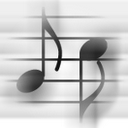
\includegraphics[width=1cm]{logos/brahms-300dpi.png}}
\label{Brahms}\acc{Wikipedia} zählt \acc{Brahms} zu den \enquote{Sequenzern},
die \enquote{[\ldots] neben ihrem Hauptanwendungsfeld der Audio- und
MIDI-Bearbeitung auch Notensatzfunktionalitäten
(beinhalten)}.\footcite[vgl.][\nopage wp]{WpedNotensatz2019a} Wir sind geneigt,
von 'Geistersoftware' zu sprechen:

Das Programm \acc{Brahms} wird in einer älteren Sichtung auf ein
Sourceforgeprojekt verlinkt\footcite[vgl.][\nopage wp]{Callon2009a}, in der
aktuelleren aber nicht.\footcite[vgl.][\nopage wp]{WpedNotensatz2019a}
Suchmaschinen beantworten den Request '\texttt{brahms musicsoftware}' im
Wesentlichen mit obigen Listen, deren Duplikate und dem
Sourceforgeprojekt.\footnote{$\rightarrow$
\href{https://www.google.com/search?q=brahms+musicsoftware}
{https://www.google.com/search?q=brahms+musicsoftware} (RDL 20190209)} Die
Homepage dieses \acc{Brahms-Sourceforge-Projektes} nutzt dann -- beruhigender-
und letztlich irreführenderweise -- ein Logo mit Noten.\footcite[vgl.][\nopage
wp]{Brahms2013a} Dennoch hat (dieses) \acc{Brahms} (von sich aus) nichts mit
Musik zu tun: es sei ein \enquote{[\ldots] Modular Execution Framework (MEF) for
executing integrated systems built from component software processes}, ein
\enquote{SystemML-ready execution client}.\footcite[vgl.][\nopage
wp]{Brahms2013b} Mittlerweile gibt es dazu ein neueres Github-Repository, das
per 'Fork' aus dem Sourceforgeprojekt entstanden ist. Und unter Github
beschreibt sich \acc{Brahms} -- direkt und ganz ohne Notenlogo -- als
\enquote{simulation execution engine}.\footcite[vgl.][\nopage wp]{Brahms2018a}

Tatsächlich ist (dieses) \acc{Brahms} kein Sequencer mit Notensatzfunktion. Und
wenn es solch ein Programm früher einmal gegeben hat -- wir vermuten eher, dass
das Logo und die Beschreibung frühere Begutachter in die Irre führte --, dann
sind die Repositories durcheinander geraten. Oder aber das richtige Notensatz-
und Sequencerprogramm \acc{Brahms} wird so versteckt gepflegt, dass auch der
unbedarfte Musikwissenschaftler es nicht einfach und schnell genug finden wird.
So läuft alles auf dasselbe hinaus: heute ist \acc{Brahms} in dieser Funktion
nicht nutzbar.


% this is only inserted to eject fault messages in texlipse
%\bibliography{../bib/literature}
 

% mycsrf 'for beeing included' snippet template
%
% (c) Karsten Reincke, Frankfurt a.M. 2012, ff.
%
% This text is licensed under the Creative Commons Attribution 3.0 Germany
% License (http://creativecommons.org/licenses/by/3.0/de/): Feel free to share
% (to copy, distribute and transmit) or to remix (to adapt) it, if you respect
% how you must attribute the work in the manner specified by the author(s):
% \newline
% In an internet based reuse please link the reused parts to mycsrf.fodina.de
% and mention the original author Karsten Reincke in a suitable manner. In a
% paper-like reuse please insert a short hint to mycsrf.fodina.de and to the
% original author, Karsten Reincke, into your preface. For normal quotations
% please use the scientific standard to cite
%


%% use all entries of the bibliography

\subsubsection{Canorus ($\bigstar\bigstar\bigstar$)}

\label{Canorus}\acc{Canorus} ist ein Notensatzprogramm\footcite[vgl.][\nopage
wp]{Canorus2019a}, das gelegentlich auch als Nachgolger von \acc{NoteEdit}
gehandelt wird.\footcite[vgl.][\nopage wp]{WpedCanorus2019a} Die vorletzte
Version (0.7.2) aus dem Jahr 2015 wurde noch als \enquote{leichtgewichtige
Alternative} zu umfangreicheren Notensatzprogrammen
bezeichnet.\footcite[vgl.][\nopage wp]{Kreussel2015a} Der letzte Releasekandidat
(0.7.3) stammt vom Juni 2018.\footcite[vgl.][\nopage wp]{Canorus2019b} Reviews
der neueren Version stehen noch aus.\footnote{Stand 01/2019} Vom Typ her gehört
\acc{Canorus} zu den graphischen Editoren: es erlaubt die Bearbeitung von Noten,
ohne Text 'programmieren' zu müssen.

Die Homepage von \acc{Canorus} ist die
Sourceforge-Projektseite.\footcite[vgl.][\nopage wp]{Canorus2019a} Aktuell wird
das Programm nicht in allen Distributionen angeboten\footnote{so nicht in Ubuntu
18.04}; externe Pakete gibt es eher für ältere
Programmsammlungen.\footcite[vgl.][\nopage wp]{RepoCanorus2019a} Dies dürfte
einen einfachen Grund haben: Der -- von 2019 aus gesehene -- vorletzte
veröffentlichte Release-Candidat 0.7.2 stammte aus dem Jahr 2015, der letzte aus
2018.\footcite[vgl.][\nopage wp]{Canorus2019b} Über drei Jahre tat sich -- von
außen gesehen - in Sachen Weiterentwicklung also wenig. In der Opensourcewelt
ist das üblicherweise ein Zeichen dafür, dass das Projekt 'eingeschlafen'
ist.\footnote{Auch vor 2015 soll es schon Unterbrechungen bei der Entwicklung
gegeben haben \cite[vgl.][\nopage wp]{UbuntuCanorus2014a}} Die Veröffentlichung
vom Juni 2018 kam dann zu spät für z.B. die Ubuntu 18.04, der
LTS-Distribution.\footnote{Long-Term-Service-Distributionen erscheinen seltener
(bei Ubuntu alle 2 Jahre), werden dafür aber länger mit Updates versorgt.}
Gleichwohl sind wir sicher, dass das Programm in kommenden Distributionen wieder
aufgenommen wird.

So bleibt Anfang 2019 im Wesentlichen nur die Installation aus den Quellen,
falls man \acc{Canorus} nutzen will. Das sollte allerdings Programmierer und
Systemkenner nicht sehr herausfordern. Das Softwarepaket liefert eine
Readme-Datei mit, die für verschiedene Umgebungen die nötigen Befehle
auflistet.\footnote{Für Ubuntu 18.04 konnten wir verifizieren, dass die
Kompilation einfach druchläuft, wenn man die geforderten Zusatzpakete -- wie
beschrieben -- installiert.} Alternativ bleibt nur, auf die nächste
Distribution zu warten, die uns dieses Programm wieder ohne Eigenarbeit zur
Verfügung stellt.

Außer der Visualisierung am Bildschirm bietet \acc{Canorus} selbst keinen
Notensatz. Für die anderen Zwecke nutzt es \acc{LilyPond} als Backend. Oder
anders gesagt: \acc{Canorus} fungiert als graphisches Frontend für das textuell
arbeitende \acc{LilyPond}. Das, was man mit \acc{Canorus} erarbeitet, speichert
es in einem eigenen \acc{XML}-Format. Importieren kann man (gegenwärtig) 
\acc{MusicXML}- und \acc{Midi}-Dateien, exportieren auch Graphiken und
\acc{LilyPond-}Dateien.

Die Arbeitsteilung zwischen \acc{Canorus} und \acc{LilyPond} hat zwei
Konsequenzen: Zum einen reicht die Installation von \acc{Canorus} allein nicht
aus, um arbeitsfähig zu werden. Auch  \acc{LilyPond} muss systemisch
bereitgestellt werden. Und zum anderen ist das, was man am Bildschirm sieht,
letztlich nicht das, was man als druckfertige PDF-Datei erhält. Hier zunächst
unsere Referenzkadenz, wie Canorus sie als PDF generiert. Wie kaum anders zu
erwarten, ähnelt sie sehr der 'puren' \acc{LilyPond}-Ausgabe:

\begin{wrapfigure}{l}{6cm}
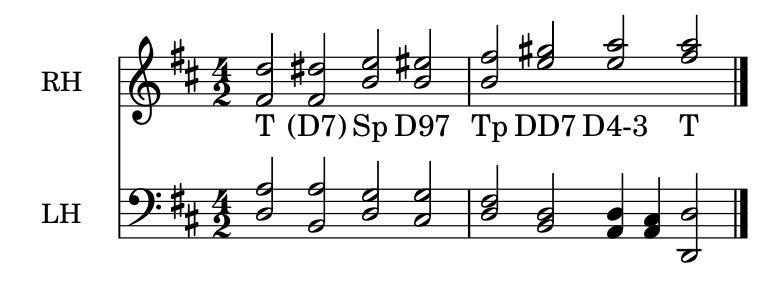
\includegraphics[width=6cm]{frontends/canorus/cadenca2-pdf-300dpi.png}
\end{wrapfigure}
Allerdings konnte der 4$\rightarrow$3 Vorhalt mit einer \Halb\ gegen zwei
gebundene \Vier\ im Bass offensichtlich nicht umgesetzt werden. Die
Funktionssymbole sind dagegen erkennbar -- ganz wie bei der Kadenz-I in der
reinen \acc{LilyPond}-Version\footnote{$\rightarrow$ S.
\pageref{LilyPondKadenzI}} -- als 'Liedtext' integriert worden. Hier wie da
gilt: ohne unsere kleine Zusatzbibliothek\footnote{$\rightarrow$ S.
\pageref{LilyPondFuncTheory}} können die Symbole der Funktionstheorie in einem
\acc{LilyPond}-Code nur in grober Form genutzt werden.

Dieser Ausgabe steht graphisch eine leicht anders gestaltete Eingabe gegenüber:
\begin{center}
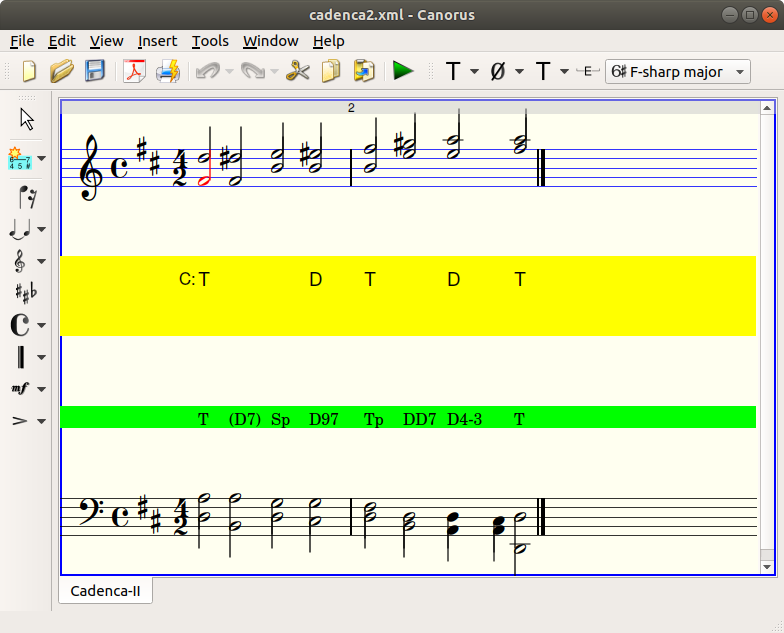
\includegraphics[width=0.9\textwidth]{frontends/canorus/cadenca2-canorus.png}
\end{center}

Man erkennt auf der linken Seite die Konzexte, die für Spezialeingaben zu
aktivieren sind. Der Modus zur Eingabe von Noten wird über das Menu aktiviert.
Oben in der Liste erscheinen die konkreten Ausformungen. Letztlich klickt man
mit der Maus dort in das Notensystem, wo die gewünschte Note erscheinen soll;
Vorzeichen werden zuvor mit \texttt{+} oder \texttt{-} aktiviert. \acc{Canorus}
ist also recht intuitiv zu bedienen. Darum fällt es nur bedingt ins Gewicht, dass
das Handbuch bei der manuelle Installation aus den Quellen heraus nicht mit
kompiliert wird.\footnote{\ldots und bis dato auch nicht im Netz zu finden ist}

Für die Eingabe von 'Liedtext' stellt \acc{Canorus} einen besonderen Modus
bereit (unten grün), den man ebenfalls im linken Randbereich aktiviert und dann
über Maus und Tastatur bedient.

Außer dem Textmodus möchte \acc{Canorus} auch noch einen Modus zur
Harmonieanalyse bereitstellen (oben, gelb). In diesem Modus kann man -- wie es
unser Bild zeigt -- in der oberen Programmleiste Funktionssymbole auswählen und
unter bestimmte Noten einfügen. Tatsächlich versucht \acc{Canorus} sogar, den
entsprechenden Akkord zu analysieren.

Damit verfolgt \acc{Canorus} einen vielversprechenden Ansatz, der über den
anderer Notensatzsysteme hinausgeht. Gleichwohl ist das Ergebnis aus drei
Gründen noch nicht produktiv nutzbar: Zum ersten werden \acc{Canorus} eigenen
Analysesymbole nicht mit gedruckt und exportiert. Zum zweiten löst die Nutzung
dieses Modus noch viele Pro\-gramm\-ab\-stürze aus. Und drittens kann man in diesem
Modus noch keine Funktionsparallelen, keine Gegenklänge und keine
Doppeldominaten ausdrücken.\footnote{Die angebotene Alternative der
Zwischendominante funktioniert nicht zuverlässig.} Darum ist dieses sehr
innovative Verfahren für den heutigen Musikwissenschaftler praktisch nicht
verwendbar.

Der \acc{LilyPond}-Code, den \acc{Canorus} exportiert, kann dagegen schon heute
gut weiterverarbeitet werden. Er ist -- sofern man auf die eigene und die
\acc{Canorus}-Harmonieanalyse verzichtet -- gut strukturiert, lesbar und
reproduzierbar\footnote{$\rightarrow$ S.\pageref{ExportVerifikation}}
korrekt.\footnote{Aus Platzgründen verzichten wir auf den erneuten Abdruck des
\acc{LilyPond}-Codes} Ohne eine textuelle Nachbearbeitung in Sachen
Harmonieanalyse wird er aber für den Musikwissenschaftler nur bedingt sinnvoll
sein.

So geben wir dem Programm 3 von 5 Sternen: In Maßen kann es jetzt bereits als
Frontend für \acc{LilyPond} verwendet werden, es ist vielversprechend, wird
aktuell gepflegt und erfüllt die Basisanforderungen. Als $\beta$-Version ist es
aber -- dem eigenen Anspruch gemäß -- von der Funktionalität und von der
Stabilität her ebenso noch begrenzt, wie vom Handling. Praktisch wird
\acc{Canorus} momentan allenfalls für den Musikwissenschaftler als
\acc{LilyPond}-Frontend in Frage kommen, der bereits mit \acc{Canorus} vertraut
ist.


% this is only inserted to eject fault messages in texlipse
%\bibliography{../bib/literature}
 

% mycsrf 'for beeing included' snippet template
%
% (c) Karsten Reincke, Frankfurt a.M. 2012, ff.
%
% This text is licensed under the Creative Commons Attribution 3.0 Germany
% License (http://creativecommons.org/licenses/by/3.0/de/): Feel free to share
% (to copy, distribute and transmit) or to remix (to adapt) it, if you respect
% how you must attribute the work in the manner specified by the author(s):
% \newline
% In an internet based reuse please link the reused parts to mycsrf.fodina.de
% and mention the original author Karsten Reincke in a suitable manner. In a
% paper-like reuse please insert a short hint to mycsrf.fodina.de and to the
% original author, Karsten Reincke, into your preface. For normal quotations
% please use the scientific standard to cite
%


%% use all entries of the bibliography

\subsubsection{Denemo}


% this is only inserted to eject fault messages in texlipse
%\bibliography{../bib/literature}
 

% mycsrf 'for beeing included' snippet template
%
% (c) Karsten Reincke, Frankfurt a.M. 2012, ff.
%
% This text is licensed under the Creative Commons Attribution 3.0 Germany
% License (http://creativecommons.org/licenses/by/3.0/de/): Feel free to share
% (to copy, distribute and transmit) or to remix (to adapt) it, if you respect
% how you must attribute the work in the manner specified by the author(s):
% \newline
% In an internet based reuse please link the reused parts to mycsrf.fodina.de
% and mention the original author Karsten Reincke in a suitable manner. In a
% paper-like reuse please insert a short hint to mycsrf.fodina.de and to the
% original author, Karsten Reincke, into your preface. For normal quotations
% please use the scientific standard to cite
%


%% use all entries of the bibliography

\subsubsection{EasyABC ($\bigstar\bigstar\bigstar\bigstar$)}

\parpic(2.5cm,1cm)[r][t]{
\includegraphics[width=2.5cm]{logos/easyabc-300dpi.png}}
\label{EasyABC}Seine Repositoryseite sagt von \acc{EasyABC}, es sei in Python
geschriebenes Notensatzprogramm, das für die graphische Darstellung auf das
Kompatibilitätsframework \acc{WxWidgets}
zurückgreife.\footnote{\cite[vgl.][\nopage wp]{EasyAbc2017a}. Die zu startende
Datei \texttt{easyabc.py} lizenziert das Programm im Header unter der GPL-3.0.
Damit ist es freie Software.} Die letzte Version stammt vom Mai
2018.\footcite[vgl.][\nopage wp]{EasyAbc2017c} Das Open Source Projekt pflegt
außerdem eine Projekthomepage, die Installationsoptionen
auflistet.\footcite[vgl.][\nopage wp]{EasyAbc2017b} Neben diesen beiden
Anlaufpunkten existiert noch die (veraltete) Homepage des ursprünglichen
Programmierers.\footcite[vgl.][\nopage wp]{Liberg2015a} Vom Typ her gehört
\acc{EasyABC} zu den semi-graphischen Editoren.

(Aktuelle) Distributionen werden \acc{EasyABC} eher nicht mit
anbieten.\footnote{Ubuntu 18.04 jedenfalls offeriert kein entsprechendes Paket.}
Denn -- laut \acc{EasyABC} Installationsanleitung -- gäbe es intendiert keine
entsprechenden Installations- oder Binärpakete: \acc{EasyABC} solle per Shell --
über den Befehl \texttt{python easy\_abc.py} -- direkt aus dem heruntergeladenen
Ordner mit den Softwarequellen gestartet werden, damit das Programm all seine
Resourcen finde.\footnote{Das Quellpaket enthält eine Linuxanleitung
(\texttt{using\_EasyABC\_in\_Windows.txt}) und eine Windowsanleitung
(\texttt{using\_EasyABC\_in\_Linux.txt}), die jeweils auflisten welche
Zusatzpakete installiert sein müssen, bevor man \acc{EasyABC} erfolgreich
starten kann. Ubuntu 18.04 Nutzer müssen bei der Abarbeitung der Liste
aufpassen: Python3 ist Distributionsstandard, während Python2.7 nur 'nebenbei'
angeboten wird. Die letzte Version von \acc{EasyABC} verlangt aber noch
Python2.7 und das dazu passende wx-Paket. Deshalb gilt es bei Ubuntu 18.04, die
Python3-Module so weit als möglich zu deinstallieren, bis der Befehl
\texttt{python --version} eine 2.7-Version ausgibt. Danach reicht es, das
Kommando \texttt{sudo apt-get install python-wxgtk-media3.0}
abzusetzen. Anschließend kann man \acc{EasyABC} erfolgreich starten.}

Nach dem Start bietet sich dem 'Notenschreiber' ein viergeteiltes Fenster an: Im
unteren rechten Bereich notiert der Komponist, Arrangeur oder
Musikwissenschaftler seine Noten im \acc{ABC}-Format. Im oberen rechten Bereich
wird daraus -- on the fly -- der entsprechende Notentext abgeleitet und
angezeigt. Der obere linke Teil des Fensters listet die offenen 'Songs' auf. Und
der untere linke Fensterteil enthält den Clou des Ganzen: einen -- auf die
Cursorposition im Notentext bezogenen -- kontextsensitiven 'Next-Steps'-Bereich,
in dem -- direkt per Klick ausführbar -- aufgelistet wird, was an der fraglichen
Stelle wie modifiziert werden kann. Für unsere Referenzkadenz II, die
\acc{EasyABC} in den Grenzen des Backens erfolgreich darstellen kann, sähe das
so aus:

\begin{center}
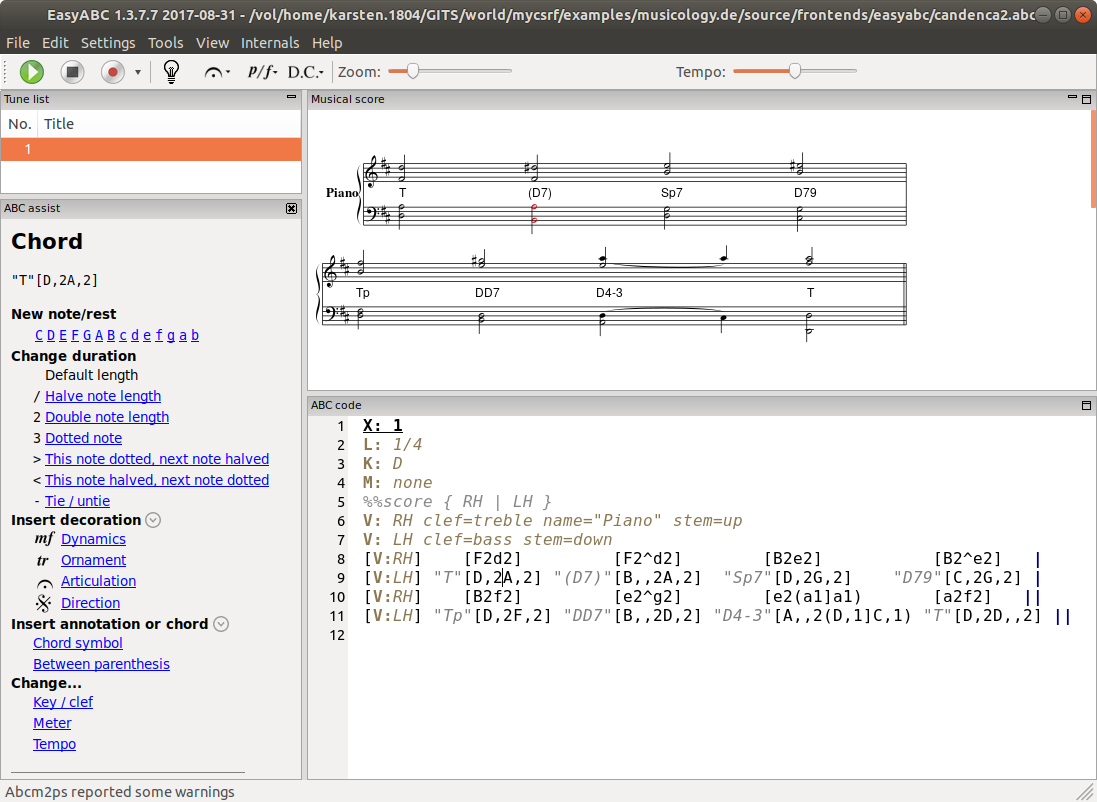
\includegraphics[width=0.9\textwidth]{frontends/easyabc/easyabc-cadenca2-300dpi.png}
\end{center}

Beim kontextsensitiven Editieren setzt man den Cursor im rechten unteren
Editorfeld in einen 'Akkord' bzw. auf eine 'Note' -- in unserem Beispiel Zeile
9, \texttt{[D,2A,2]} --, den oder die das System in der rechten oberen
Visualisierung rot einfärbt. Dieser per Cursor ausgewählte Bereich wird im
linken unteren Fensterteil analysiert und beschrieben, bevor darunter all die
Modifikationen und Erweiterungen aufgelistet werden, die an dieser Stelle in
diesem Kontext von der \acc{ABC}-Syntax her möglich sind. \acc{EasyABC} bietet
damit eine zukunftsweisende und trickreiche 'Code-Completion' an, die die
Tipparbeit wirklich zu vereinfach vermag.

Schließlich bliebe zu erwähnen, dass man das, was man im Editorfenster
eingegeben hat, als \acc{ABC}-Code speichern oder als PDF-, MIDI, MusicXML- oder
HTML-Datei exportieren kann. Außerdem bietet \acc{EasyABC} bei gelungener
MIDI-Integration die Möglichkeit, das eingegebene auch zu hören.

In Verbindung mit den Konvertern bietet \acc{EasyABC} den Musikwissenschaftlern
als textbasierter Editor mit automatisierter Visualisierung also ein sehr gut zu
nutzendes Frontend für die \acc{ABC}-Notationsmethode.

% this is only inserted to eject fault messages in texlipse
%\bibliography{../bib/literature}
 

% mycsrf 'for beeing included' snippet template
%
% (c) Karsten Reincke, Frankfurt a.M. 2012, ff.
%
% This text is licensed under the Creative Commons Attribution 3.0 Germany
% License (http://creativecommons.org/licenses/by/3.0/de/): Feel free to share
% (to copy, distribute and transmit) or to remix (to adapt) it, if you respect
% how you must attribute the work in the manner specified by the author(s):
% \newline
% In an internet based reuse please link the reused parts to mycsrf.fodina.de
% and mention the original author Karsten Reincke in a suitable manner. In a
% paper-like reuse please insert a short hint to mycsrf.fodina.de and to the
% original author, Karsten Reincke, into your preface. For normal quotations
% please use the scientific standard to cite
%


%% use all entries of the bibliography

\subsubsection{Elysium ($\bigstar\bigstar\bigstar\bigstar$)}

\label{Elysium}\acc{Elysium} fungiert als Frontend für \acc{LilyPond}, ohne ein
eigenständiger Editor zu sein. Es wird vielmehr zusammen mit \acc{Eclipse}
genutzt, einer integrierten Entwicklungsumgebung, deren Funktionalität erst über
die Integration von Plugins entsteht. Entwickelt und gepflegt wird diese
IDE\footnote{Integratet Development Environment} von der \acc{Eclipse
Foundation}.\footcite[vgl.][\nopage wp]{Eclipse2018a} Sie bietet die
verschiedensten vorkonfigurierten Pakete an, zusammengestellt für die
unterschiedlichsten Zwecke und ausgelegt auf die gängigsten Betriebssysteme. In
unserem Fall reicht das einfache Standardpaket \enquote{Eclipse IDE for Java
Developers}.\footcite[vgl.][\nopage wp]{Eclipse2018b}

Ein Plugin, das zu installieren in unserem Kontext lohnt, wäre z.B.
\acc{{\TeX}lipse}: es macht \acc{Eclipse} zu einem exezellenten 'Editor' für
\LaTeX-Texte.\footcite[vgl.][\nopage wp]{TeXlipse2019a}

Das für unsere Zwecke entscheidende Plugin ist \acc{Elysium}. Es wird aus
Eclipse heraus vom \enquote{Eclipse-Marketplace} heruntergeladen und
installiert.\footcite[vgl.][\nopage wp]{Harmath2019a} Sein Schöpfer -- Dénes
Harmath -- nennt seine Erweiterung die \enquote{LilyPond IDE für
Eclipse}.\footcite[vgl.][\nopage wp]{Harmath2019b} Der Name \acc{Elysium}
verweise auf \acc{Eclipse} und \acc{.ly}, der Extension von LilyPond-Dateien und
stehe für eine \enquote{himmlische} Verbindung: Schließlich sei beides
Open-Source-Software, wobei \enquote{[\ldots] writing complex scores with
LilyPond inevitably requires a more agile, more managed approach than a simple
command line and plain text editor}. Und eben das unterstütze \acc{Eclipse} als
bewährte Entwicklungsumgebung schon von sich aus.\footcite[vgl.][\nopage
wp]{Harmath2019d} Dem entsprechend ist \acc{Elysium} als freie Software
quelloffen unter der \acc{Eclipse Public License} publiziert
worden\footcite[vgl.][\nopage wp]{Harmath2018a}. Das System werde -- wie es
heißt -- in vier Schritten bereitgestellt: Sofern es die eigene Distribution
nicht schon mit sich bringe, installiere man zuerst auf die gewohnte Weise
\acc{LilyPond}, dann \acc{Eclipse} und von da aus das Plugin
\acc{Elysium}.\footcite[vgl.][\nopage wp]{Harmath2019c} Alle Varianten liefen
bei uns problemlos durch.

Von seinen Eigenschaften her ist \acc{Elysium} ein semi-graphischer Editor: man
gibt -- Editor gestützt -- den gewünschten \acc{LilyPond}-Code ein und bei jeder
Sicherung der Quelldatei werden die entsprechende MIDI- und die zugehörige
PDF-Datei kompiliert und angezeigt.\footcite[vgl.][\nopage wp]{Harmath2019e} Auf
diese Weise kann \acc{Elysium} auch mit unser Referenzkadenz II problemlos
umgehen, als \acc{LilyPond}-Frontend sogar inklusive unser kleinen
Zusatzbibliothek:

\begin{center}
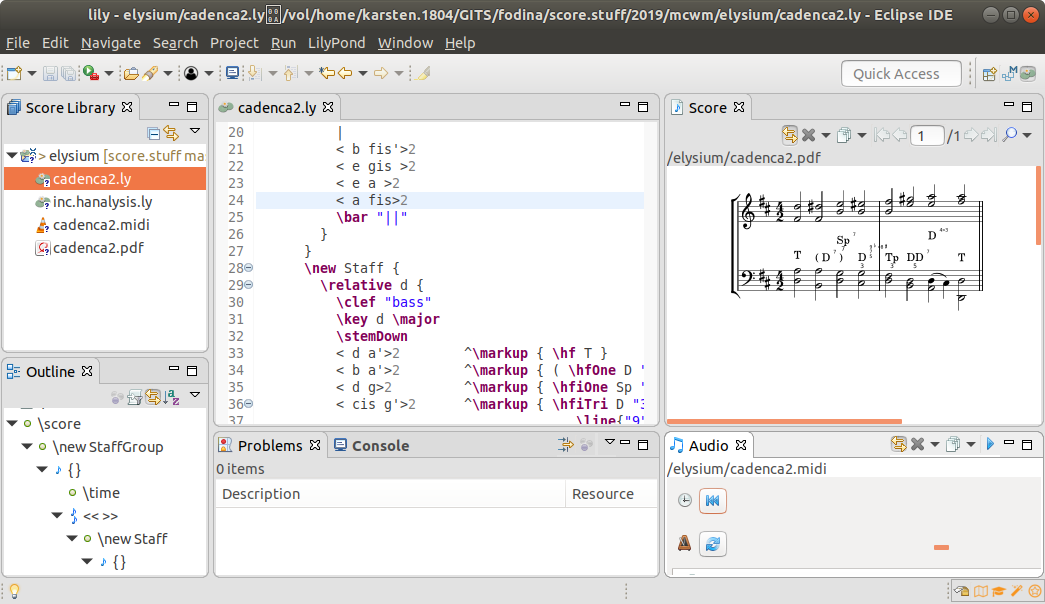
\includegraphics[width=0.9\textwidth]{frontends/elysium/elysium-cadenca2-300dpi.png}
\end{center}

Die \acc{LilyPond}-Perspektive, die das \acc{Elysium}-Plugin mitbringt, enthält
in der oberen Mitte den eigentlichen \acc{LilyPond}-Editor. Er nutzt
Syntaxhighlighting und bietet-- über die Eclipse-Menues -- den bei \acc{Eclipse}
gewohnten Programmiersupport. Links davon findet sich -- entsprechenend -- eine
Liste der Projekte und ihrer Dateien. Und darunter wird die Struktur der Datei
abgebildet, die gerade editiert wird. Auf der rechten oberen Seite erscheint
dann nach jeder Sicherung des eingegebenen Codes der Notentext, der daraus
erzeugt werden kann. Und der rechte untere Bereich bietet einen MIDI-Player, mit
dem man sich seine generierte Musik anhören kann.

Zwei Kleinigkeiten können bei der Nutzung verwirren: 

Zum ersten muss man das 'Noten'-Fenster und das \acc{MIDI}-Player-Fenster an
eine geöffnete Datei 'binden', wenn man den Notentext sehen und hören möchte.
Dazu nutzt man die gelben Pfeile.

Außerdem erwartet \acc{Elysium}, dass in der Projektspalte des Eclipsemenues die
Option 'build automatically' aktiviert ist. Nur dann nämlich generiert
\acc{Elysium} unter Rückgriff auf das installierte \acc{LilyPond}-Backend
automatisch die zurghörige PDF-Datei und -- sofern im Code mit \texttt{MIDI\{\}}
aktiviert -- die entsprechendene MIDI-Datei, die dann im rechten oberen und
unteren Bereich dargestellt werden.

Nun gibt es durchaus Gründe, nicht alle Projekte immer automatisch bilden zu
lassen\footnote{So schreiben wir z.B. den Text, den Sie gerade lesen, mit
\acc{Elcipse} und \acc{Texlipse}. Gemeinsam wissen wir aber bereits, dass unser
Text nicht standardmäßig prozessiert werden darf, weil ja \texttt{lilypond-book}
immer zuerst ausgeführt werden muss und den eigentlichen \LaTeX-Text erst
generiert.} Will man solche Projekte mit manuellem Anstoß und die
Lilypond-Projekte, die die automatische Abarbeitung fordern, gemeinsam offen
halten, wird man Auto-Build-Funktionen je nach Bedarf an und abschalten müssen
und die Fehlermeldungen souverän ignorieren, von denen man weiß, daß sie
'natürlich' sind. Alternativ kann man natürlich eine weitere Eclipse-Instanz mit
anderem Workspace starten.

Insgesamt erhält man mit \acc{Elysium} eine verlässlich solide Umgebung zur
Entwicklung von \acc{LilyPond} basierten Noten, die insbesondere denjenigen ans
Herz wachsen wird, die eh schon mit \acc{Eclipse} arbeiten.

% this is only inserted to eject fault messages in texlipse
% \bibliography{../bib/literature}
 

% mycsrf 'for beeing included' snippet template
%
% (c) Karsten Reincke, Frankfurt a.M. 2012, ff.
%
% This text is licensed under the Creative Commons Attribution 3.0 Germany
% License (http://creativecommons.org/licenses/by/3.0/de/): Feel free to share
% (to copy, distribute and transmit) or to remix (to adapt) it, if you respect
% how you must attribute the work in the manner specified by the author(s):
% \newline
% In an internet based reuse please link the reused parts to mycsrf.fodina.de
% and mention the original author Karsten Reincke in a suitable manner. In a
% paper-like reuse please insert a short hint to mycsrf.fodina.de and to the
% original author, Karsten Reincke, into your preface. For normal quotations
% please use the scientific standard to cite
%

\subsubsection{Free Clef ($\bigstar$)}

\label{FreeClef}\acc{Free Clef} bezeichnet sich selbst als \enquote{lightweight
notation editor}, der es seinen Nutzern erlaube, Musik zu schreiben und im
MusicXML-Format zu exportieren. Die letzte veröffentlichte Version stammt vom
Juni 2008, es handelt sich allerdings noch um eine
\acc{Beta}-Version.\footcite[vgl.][\nopage wp]{FreeClef2008a}

Moderne Distributionen bieten keine Binärpakete für \acc{Free Clef}
an.\footnote{Jedenfalls nicht Ubuntu 18.04.} Der Sourcecode kann von der
Projektseite heruntergeladen werden. Allerdings verlangt diese Software bei
einer Installation aus den Quellen heraus die Kompatibilitätsbibliothek
\acc{wxwidgets} in der Version 2.8. Aktuell stellen besagte Distirbutionen aber
nur die Version 3.x bereit, weil sie selbst ja bereits auf GNOME-3 und damit auf
GTK-3 basieren.

Damit scheidet \acc{Free Clef} als Notensatzsystem aktuell (noch) aus. Dass er
in den Quellen vorliegt und das GNU-automake/autoconf-System benutzt, macht eine
'Wiederbelebung' nicht unmöglich. Dies ist uns -- wieder einmal -- wenigstens
einen Stern wert.



% this is only inserted to eject fault messages in texlipse
%\bibliography{../bib/literature}


% mycsrf 'for beeing included' snippet template
%
% (c) Karsten Reincke, Frankfurt a.M. 2012, ff.
%
% This text is licensed under the Creative Commons Attribution 3.0 Germany
% License (http://creativecommons.org/licenses/by/3.0/de/): Feel free to share
% (to copy, distribute and transmit) or to remix (to adapt) it, if you respect
% how you must attribute the work in the manner specified by the author(s):
% \newline
% In an internet based reuse please link the reused parts to mycsrf.fodina.de
% and mention the original author Karsten Reincke in a suitable manner. In a
% paper-like reuse please insert a short hint to mycsrf.fodina.de and to the
% original author, Karsten Reincke, into your preface. For normal quotations
% please use the scientific standard to cite
%


%% use all entries of the bibliography

\subsubsection{Frescobaldi ($\bigstar\bigstar\bigstar\bigstar\bigstar$)}

\parpic(1cm,1cm)[r][t]{
\includegraphics[width=1cm]{logos/frescobaldi-300dpi.png}}
\label{Frescobaldi}\acc{LilyPond} 'bewirbt' \acc{Frescobaldi} als
\enquote{leichtgewichtigen} und \enquote{mächtigen LilyPond Musik- und
Texteditor mit vielen für die Arbeit mit LilyPond nützlichen Fähigkeiten}.
Besonders hervorgehoben wird \enquote{die beidseitige Verknüpfung zwischen dem
LilyPond Code und der dargestellten Musik} über den \enquote{‚point-and-click‘
per Maus}.\footcite[vgl.][\nopage wp]{LilyPond2018g} Daraus ergibt sich sofort,
was \acc{Frescobaldi} ist: ein Editor, bei dem der Komponist oder
Musikwissenschaftler \acc{LilyPond}-Code eingibt und als Feedback den
visualisierten Notentext erhält: \acc{Frescobaldi} gehört zu den
semi-graphischen Frontends.

Das Programm ist freie, unter GPL lizensierte Software, dessen Code auf Github
ge\-hos\-tet und zum Download bereitgestellt wird.\footnote{\cite[vgl.][\nopage
wp]{Frescobaldi2019a}. Dem entsprechend enthält das Repository unter dem
Dateinamen \texttt{COPYING} die GPL-2.0 Lizenz.} Als Applikation wird
\acc{Frescobald} auf einer umfangreichen Site vorgestellt\footcite[vgl.][\nopage
wp]{Frescobaldi2017a}, die auch den Download und die Installation beschreibt
\footcite[vgl.][\nopage wp]{Frescobaldi2015a} und ein ausführliches 'Manual'
mitliefert.\footcite[vgl.][\nopage wp]{Frescobaldi2012a} Gängige Distributionen
enthalten entsprechende Programmpakete, sodass die aufwendigere Installation aus
den Quellen in der Regel nicht notwendig ist.\footcite[vgl.][\nopage
wp]{UbuntuFrescobaldi2016a}

\acc{Frescobaldi} vermag \acc{LilyPond}-Dateien direkt zu lesen und erlaubt den
konvertierenden Import von \acc{MusicXML}-, \acc{MIDI-} und \acc{ABC}-Dateien.
Als Export bietet sein Menue auf den ersten Blick 'nur' die Sicherung als
HTML-Seite an. Allerdings nutzt \acc{Frescobaldi} ja das ganze
\acc{LilyPond}-Backend. Das heißt, dass aus einer \acc{LilyPond}-Datei implizit
'immer' auch die korrespondierende \acc{MIDI}-Datei und die entsprechende
\acc{PDF}-Datei erzeugt werden.\footnote{Dies allerdings nur dann, wenn deren
Bildung über die in den Code eingebetteten 'Kommandos'
\texttt{{\textbackslash}midi \{ \}} bzw.
\texttt{{\textbackslash}layout \{ \}} mit angestoßen werden. In diesem Fall
werden die abgeleiteten Dateien unter gleichem Namenskern mit entsprechender
Datei-Extension neben der \texttt{.ly}-Datei abgelegt.} Initial muss das
Generieren dieser Artefakte für ein geladenes oder editiertes Musikstück über
das \acc{LilyPond}-Icon angestoßen werden. Unter der Rubrik \acc{Tools} kann man
dann eine Midiplayer einblenden lassen, der das Stück -- bei gelungener
Soundaktivierung -- hörbar macht.\footnote{In der Regel muss man
\acc{Frescobaldi} über den Dialog \acc{Edit/Prefrences/Midi} noch mitteilen,
über welches MIDI-Backendsystem es die Midi-Töne akkustisch generieren lassen
soll. Unter GNU/Linux respektive Ubuntu kann man z.B. \acc{timidity} über das
Shell-Kommando \texttt{timidity -iA} als Server starten, dessen geöffnete Ports
in dem \acc{Frescobaldi}-Dialog angezeigt werden, wenn man \acc{timidity} vor
\acc{Frescobaldi} gestartet hat.}

Seiner Natur nach kann \acc{Frescobaldi} unsere Referenzkadenz II direkt aus als
\acc{LilyPond}-Datei einlesen und auch unmittelbar unsere kleine
Zusatzbibliothek interpretieren, über die wir die Symbole der Harmonieanalyse in
den Notentext integrieren. Sobald man einmal das \acc{LilyPond}-Icon in der
oberen Leiste angeklickt hat, werden die entsprechenden \acc{Midi-} und die
\acc{PDF}-Dateien generiert und angezeigt:

\begin{center}
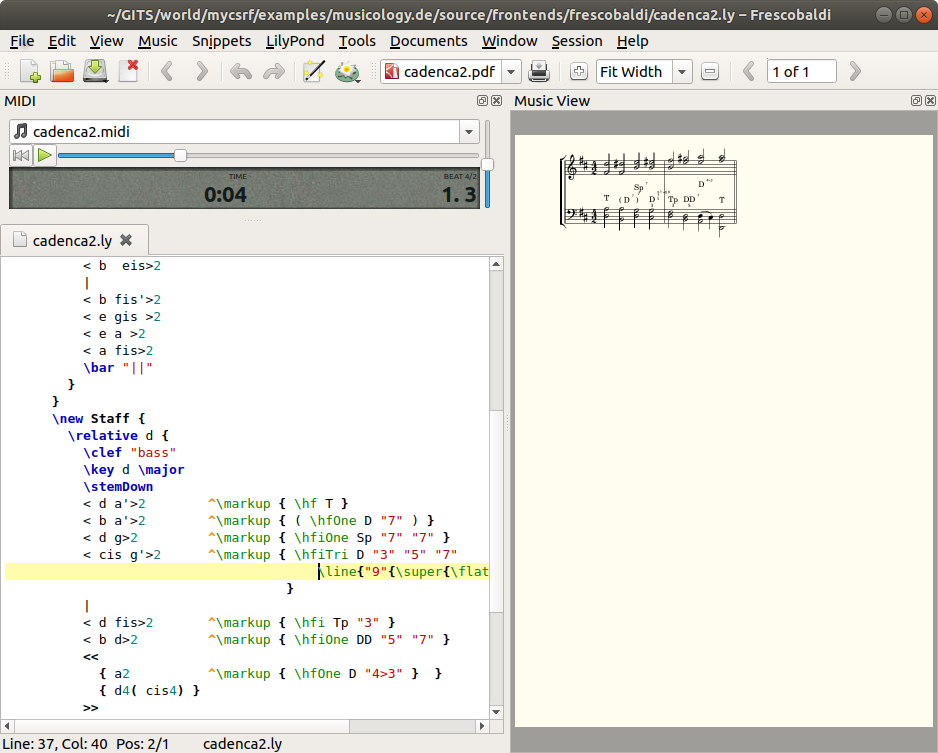
\includegraphics[width=0.9\textwidth]{frontends/frescobaldi/frescobaldi-cadenca2-300dpi.png}
\end{center}

Auf der linken unteren Seite editiert man den \acc{LilyPond}-Text, unterstützt
durch ein gelungenes Syntaxhighlighting und durch Menue-Befehle, die komplexere
Eingaben zusammenfassen. Über diesem Eingabefenster erscheint das Frontend zum
Midi-Player, wenn man diesen über die Rubrik 'Tools' aktiviert hat. Und rechts
daneben wird das generiert PDF angezeigt.

Wenn wir \acc{Elysium} mit vier Sternen ausgezeichnet haben, dann ist es nur
fair, an \acc{Frescobaldi} fünf Sterne zu vergeben: Beide Systeme gehören zur den
semi-graphischen Editoren, beide nutzen dasselbe Backend und dasselbe
Arbeitsprinzip. \acc{Frescobalid} unterstützt seinen Nutzer allerdings ein wenig
eleganter und zielgerichteter.
% this is only inserted to eject fault messages in texlipse
%\bibliography{../bib/literature}
 

% mycsrf 'for beeing included' snippet template
%
% (c) Karsten Reincke, Frankfurt a.M. 2012, ff.
%
% This text is licensed under the Creative Commons Attribution 3.0 Germany
% License (http://creativecommons.org/licenses/by/3.0/de/): Feel free to share
% (to copy, distribute and transmit) or to remix (to adapt) it, if you respect
% how you must attribute the work in the manner specified by the author(s):
% \newline
% In an internet based reuse please link the reused parts to mycsrf.fodina.de
% and mention the original author Karsten Reincke in a suitable manner. In a
% paper-like reuse please insert a short hint to mycsrf.fodina.de and to the
% original author, Karsten Reincke, into your preface. For normal quotations
% please use the scientific standard to cite
%

\subsubsection{Jniz (-)}

\label{Jniz}Ein ganz spezielles Programm ist \acc{Jniz}. Es bezeichnet sich
selbst als \enquote{support tool} für Komponisten, das es erlaube, mehrstimmige
Stücke gemäß der klassischen Regeln (semi-automatisch) zu
harmonisieren.\footcite[vgl.][\nopage wp]{Grandjean2019a} Das zum Download
angebotene Programm kann per \texttt{java -jar jnizpro.jar} gestartet werden.
Die letzte wirklich lauffähige Version stammt aus dem Jahr 2016, die aktuellste
von 2019.\footcite[vgl.][\nopage wp]{Jniz2019b} Dazu gibt es ein
Tutorial.\footcite[vgl.][\nopage wp]{Grandjean2019c}

Das Programm erlaubt keinen Import und lädt nur Dateien im eigenen Format.
Kadenzen können in einfacher Form gebildet, allerdings nur sehr bedingt manuell
gestaltet werden.\footnote{Es ist uns nicht gelungen, die Referenzkadenz II
einzugeben.} Der angebotene Export als \acc{MusicXML-}, \acc{LilyPond-},
\acc{MIDI-} oder \acc{PDF-}Datei ist darum nur bedingt hilfreich.

Speziell ist dieses Programm nicht nur seines Ansatzes wegen, sondern auch ob
seiner Lizensierung. Hier verbietet der Autor, das Programm zu verkaufen. Und
mehr noch, er untersagt auch, seine Quellen weiterzugeben: \enquote{You do not
have the right to sell, distribute Jniz or use its sources under penalty of
law.}\footcite[vgl.][\nopage wp]{Grandjean2019b} Damit unterläuft es seine
'Selbstklassifikation' als freie Software. Dass es dennoch unter Sourceforge
gehostet wird, mutet merkwürdig an.\footnote{Immerhin bezeichnet sich
Sourceforge als \enquote{Open Source community resource dedicated to helping
open source projects} ($rightarrow$ \href{https://sourceforge.net/}
{https://sourceforge.net/}).} Noch bedenklicher aber ist die Tatsache, dass
\acc{Jniz} selbst unter der \acc{GPL} lizensierte \acc{LilyPond}-Bibliotheken
nutzt. Damit wird es zu einem abgeleiteten Werk und müsste -- des
\acc{Copyleft-Effektes} wegen -- ebenfalls unter der GPL veröffentlicht
werden.\footnote{Dies wird in den Reviews auf der Repositorysite diskutiert
(\cite[vgl.][\nopage wp]{Jniz2019a})}

Damit ist dieses Programm in unserem Kontext nicht nur funktional kaum nutzbar,
seine Nutzung ist auch lizenztechnisch bedenklich.



% this is only inserted to eject fault messages in texlipse
%\bibliography{../bib/literature}


% mycsrf 'for beeing included' snippet template
%
% (c) Karsten Reincke, Frankfurt a.M. 2012, ff.
%
% This text is licensed under the Creative Commons Attribution 3.0 Germany
% License (http://creativecommons.org/licenses/by/3.0/de/): Feel free to share
% (to copy, distribute and transmit) or to remix (to adapt) it, if you respect
% how you must attribute the work in the manner specified by the author(s):
% \newline
% In an internet based reuse please link the reused parts to mycsrf.fodina.de
% and mention the original author Karsten Reincke in a suitable manner. In a
% paper-like reuse please insert a short hint to mycsrf.fodina.de and to the
% original author, Karsten Reincke, into your preface. For normal quotations
% please use the scientific standard to cite
%


%% use all entries of the bibliography

\subsubsection{Laborejo}


% this is only inserted to eject fault messages in texlipse
%\bibliography{../bib/literature}
 

% mycsrf 'for beeing included' snippet template
%
% (c) Karsten Reincke, Frankfurt a.M. 2012, ff.
%
% This text is licensed under the Creative Commons Attribution 3.0 Germany
% License (http://creativecommons.org/licenses/by/3.0/de/): Feel free to share
% (to copy, distribute and transmit) or to remix (to adapt) it, if you respect
% how you must attribute the work in the manner specified by the author(s):
% \newline
% In an internet based reuse please link the reused parts to mycsrf.fodina.de
% and mention the original author Karsten Reincke in a suitable manner. In a
% paper-like reuse please insert a short hint to mycsrf.fodina.de and to the
% original author, Karsten Reincke, into your preface. For normal quotations
% please use the scientific standard to cite
%




\subsubsection{MusEdit (-)}

\label{MusEdit}Die neuere Sichtung von Notensatzprogrammen listet \acc{MusEdit}
schon nicht mehr\footcite[vgl.][\nopage wp]{WpedNotensatz2019a}, \acc{MusicXML}
erwähnt sie noch als \enquote{notation editor for Windows}, der schließlich
freie Software geworden sei\footcite[vgl.][\nopage wp]{MusicXML2018b}. Die
ursprüngliche Domain \texttt{http://www.musedit.com/} ist nicht mehr erreichbar.
Die Software wird über eine Ersatzhomepage 'vertrieben'. Dort  bekennt er Autor
unten, dass er die Software seit 2011 nicht mehr pflegen könne. Und oben
'kündigt' er an, dass die Software 'bald' Open-Source-Software
werde\footcite[vgl.][\nopage wp]{Rogers2011a} -- was aber offensichtlich
(bisher) nicht geschehen ist.

Unabhängig davon, wie gut dieses Programm früher einmal mit
\acc{MusicXML}-Dateien umgehen konnte, heute ist es (für Musikwissenschaftler)
keine Alternative mehr -- und schon gar nicht für diejenigen, die Wert auf freie
Software legen. Für den Ehrenstern hat uns das nicht gereicht.

% this is only inserted to eject fault messages in texlipse
%\bibliography{../bib/literature}
 

% mycsrf 'for beeing included' snippet template
%
% (c) Karsten Reincke, Frankfurt a.M. 2012, ff.
%
% This text is licensed under the Creative Commons Attribution 3.0 Germany
% License (http://creativecommons.org/licenses/by/3.0/de/): Feel free to share
% (to copy, distribute and transmit) or to remix (to adapt) it, if you respect
% how you must attribute the work in the manner specified by the author(s):
% \newline
% In an internet based reuse please link the reused parts to mycsrf.fodina.de
% and mention the original author Karsten Reincke in a suitable manner. In a
% paper-like reuse please insert a short hint to mycsrf.fodina.de and to the
% original author, Karsten Reincke, into your preface. For normal quotations
% please use the scientific standard to cite
%


%% use all entries of the bibliography

\subsubsection{Musescore ($\bigstar$)}


% this is only inserted to eject fault messages in texlipse
%\bibliography{../bib/literature}
 

% mycsrf 'for beeing included' snippet template
%
% (c) Karsten Reincke, Frankfurt a.M. 2012, ff.
%
% This text is licensed under the Creative Commons Attribution 3.0 Germany
% License (http://creativecommons.org/licenses/by/3.0/de/): Feel free to share
% (to copy, distribute and transmit) or to remix (to adapt) it, if you respect
% how you must attribute the work in the manner specified by the author(s):
% \newline
% In an internet based reuse please link the reused parts to mycsrf.fodina.de
% and mention the original author Karsten Reincke in a suitable manner. In a
% paper-like reuse please insert a short hint to mycsrf.fodina.de and to the
% original author, Karsten Reincke, into your preface. For normal quotations
% please use the scientific standard to cite
%


%% use all entries of the bibliography

\subsection{MuX2d ($\bigstar$)}

\label{MuX2d}\acc{MuX2d} beschreibt sich als \enquote{WYSIWYM(ean) editor for
MusiXTeX}, will sagen: als \enquote{macro package for typesetting music with
TeX}, das unter der GPL veröffentlicht werde.\footcite[vgl.][\nopage
wp.]{Mux2d2000a} Ein Open-Source-\acc{MusiX\TeX}-Frontend weckt in unserem
Kontext natürlich besonderes Interesse. Die letzte Version ist allerdings schon
vor fast 20 Jahren als Release 0.2.4 erschienen.\footnote{\cite[vgl.][\nopage
wp.]{Mux2d2000b}. Auch die Projekseite gibt an, dass \acc{MuX2d} unter der GPL-2.0
distributiert werde. Es ist also freie Software.} Und sie wurde damals noch als
\enquote{quite early} bezeichnet.\footcite[vgl.][\nopage wp.]{Mux2d2000a} Beides
lässt Schlimmes erahnen.

Und in der Tat liefern gängige Distributionen keine \acc{muX2d}-Pakete mehr. Die
zu Download angeboten Binärversion verweigert mit dem Hinweis den Dienst, es
könne die \acc{libqt.so.2} nicht finden. Und die Sourcecodeversion kann nicht
kompiliert werden, weil dabei eine veraltete Version der \acc{qt}-Bibliothek
gesucht wird.

Damit scheidet für Musikwissenschaftler auch \acc{muX2D} als Editor aus, so gern
wir ihn auch angeboten hätten. Man könnte dieses Programm wohl mit einigem
Aufwand wiederbeleben. Angesichts der frühen Entwicklungsstadiums und des Alters
mag sich das aber als nicht fruchtbringend herausstellen. Einen Stern ist uns
die bloße Möglichkeit jedoch -- wie immer -- wert.
% this is only inserted to eject fault messages in texlipse
%\bibliography{../bib/literature}
 

% mycsrf 'for beeing included' snippet template
%
% (c) Karsten Reincke, Frankfurt a.M. 2012, ff.
%
% This text is licensed under the Creative Commons Attribution 3.0 Germany
% License (http://creativecommons.org/licenses/by/3.0/de/): Feel free to share
% (to copy, distribute and transmit) or to remix (to adapt) it, if you respect
% how you must attribute the work in the manner specified by the author(s):
% \newline
% In an internet based reuse please link the reused parts to mycsrf.fodina.de
% and mention the original author Karsten Reincke in a suitable manner. In a
% paper-like reuse please insert a short hint to mycsrf.fodina.de and to the
% original author, Karsten Reincke, into your preface. For normal quotations
% please use the scientific standard to cite
%


%% use all entries of the bibliography

\subsubsection{NoteEdit ($\bigstar$)}

\parpic(1.4cm,1cm)[r][t]{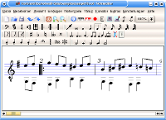
\includegraphics[width=1.4cm]{logos/noteedit-300dpi.png}}
\label{NoteEdit}Wer nach freien Notensatzprogrammen sucht, dem wird sicher auch
\acc{NoteEdit}\footcite[vgl.][\nopage wp]{Andres2002a} vorgeschlagen. Ältere
Sichtungen gehen gern auf das Programm ein\footcite[vgl.][\nopage
wp]{Roitman2007a}; manche mit affirmativem Ton\footcite[vgl.][\nopage
wp]{LinuxSoundNotation2006a}, manche ohne
\footnote{\cite[vgl.][\nopage]{Brendel2005a} - hier
\href{http://www.linux-magazin.de/ausgaben/2005/09/digitale-notenstecher/2/}
{http://www.linux-magazin.de/ausgaben/2005/09/digitale-notenstecher/2/} und
\texttt{\/3\/}}. Neuere Sichtungen bezeichnen es als
\enquote{obsolet}\footcite[vgl.][\nopage wp]{WpedNotensatz2019a}.
Der Quellcode des Programms ist allerdings auch heute noch
erreichbar\footnote{\cite[vgl.][\nopage]{NoteeditRep2014a}. Das Repository sagt,
das Programm stünde unter der GPL-2.0 Lizenz. Damit wäre es freie Software.},
eine ausführbare Version wird in der Regel aber nicht mehr angeboten, weder im
Netz, noch als Distri\-bu\-tions\-paket\footnote{jedenfalls nicht in Ubuntu
18.04.}. Gelegentlich wird erwähnt, dass spätere Entwickler von \acc{Noteedit}
schließlich zu \acc{Canorus} gewechselt seien\footnote{$\rightarrow$
\href{https://wiki.ubuntuusers.de/Canorus/}{https://wiki.ubuntuusers.de/Canorus/}
} und dass \acc{Canorus} nun der \enquote{offizielle Nachfolger} von
\acc{Noteedit} sei\footcite[vgl.][\nopage wp]{WpedCanorus2019a}.
Jedenfalls verlinkt auch sein ursprünglicher Autor \acc{NoteEdit} in seiner Vita
auf eine Homepage, die nicht mehr erreichbar ist\footnote{Offensichtlich ist
Notedit zunächst auf dem deutschen FOSS-Repository \acc{Berlios} gehostet worden
und nach dessen Einstellung nach Sourceforge migriert worden. An der Verlinkung
kann man das noch erkennen. \cite[vgl. dazu][\nopage wp]{Andres2018a}.}.

Dass der Quelltext noch zugänglich
ist\footcite[vgl.][\nopage]{NoteeditRep2014a}, löst das Problem nicht. Zwar
gehören zum Paket auch die Installationsskripte. Aber diese fordern Komponenten an,
die heute ob ihres Alters nicht mehr (so einfach) zur Verfügung stehen. Eine
direkte Installation aus den Quellen heraus misslingt also. So bleibt nur der
Schluss, dass dieses Programm vorerst nicht mehr nutzbar ist\footnote{Gleichwohl
werden die Quellen samt der GNU-make-Files ausgeliefert. Damit steht einer
Aktualisierung prinzipiell nichts im Wege. Es ist 'nur' eine Frage des
Programmier- und Konfigurationsaufwandes, bis \acc{NoteEdit} über die Aufrufe
\texttt{autoconf automake configure --prefix=/dir make make install} wieder zur
Verfügung stünde. Ob sich solch eine 'Wiederbelebung' lohnt, ist letztlich eine
Frage der Lust am Programmieren, nicht der Lust am Musizieren. }. Das ist
insofern bedauerlich, als es eines der wenigen Programme (gewesen) sein soll,
die ihren Inhalt auch als MusiX\TeX-Datei exportieren
konnten\footcite[vgl.][\nopage wp]{Roitman2007a}.

Wir geben \acc{NoteEdit} also doch noch 1 von 5 Sternen. Denn in der
Vergangenheit hat das Programm wesentlich zum Komponieren und Arrangieren mit
freier Software ermuntert.


% this is only inserted to eject fault messages in texlipse
%\bibliography{../bib/literature}
 
 
% mycsrf 'for beeing included' snippet template
%
% (c) Karsten Reincke, Frankfurt a.M. 2012, ff.
%
% This text is licensed under the Creative Commons Attribution 3.0 Germany
% License (http://creativecommons.org/licenses/by/3.0/de/): Feel free to share
% (to copy, distribute and transmit) or to remix (to adapt) it, if you respect
% how you must attribute the work in the manner specified by the author(s):
% \newline
% In an internet based reuse please link the reused parts to mycsrf.fodina.de
% and mention the original author Karsten Reincke in a suitable manner. In a
% paper-like reuse please insert a short hint to mycsrf.fodina.de and to the
% original author, Karsten Reincke, into your preface. For normal quotations
% please use the scientific standard to cite
%


%% use all entries of the bibliography

\subsubsection{NtEd ($\bigstar$$\bigstar$)}
 
\label{NtEd}Gegenwärtig trifft man im Netz unter dem Stichwort
\acc{Notensatzprogramm} auch noch auf \acc{NtEd}. Die aktuellere Übersicht
listet es ebenso\footcite[vgl.][\nopage wp]{WpedNotensatz2019a}, wie die ältere:
dort wird es unter dem Label \enquote{excellent music notation editor}
präsentiert\footcite[vgl.][\nopage wp]{LinuxSoundNotation2006a}. Über
Distributionen ist das Programm noch zugänglich\footnote{Unter Ubuntu 18.04 mit
\texttt{sudo apt-get install nted}.}. Gleichwohl wird schon darauf hingewiesen,
dass Sourcecode, Projektseite und Handbuch \enquote{seit November 2017} nicht
mehr erreichbar seien\footcite[vgl.][\nopage wp]{UbuntuNtEd2016a}.
Dazu passt, dass selbst der Autor \acc{NtEd} auf seiner
'Selbstvorstellungsseite'\footcite[vgl.][\nopage wp]{Andres2018a} auf eine
\acc{NtEd}-Homepage\footcite[vgl.][\nopage wp]{Andres2018b} verlinkt, die nicht
(mehr) aufgerufen werden kann.
 
Unsere \acc{Referenzkadenz II} kann mit \acc{NtEd} durchaus erfasst werden. Das
Handling ist gelegentlich sperrig\footnote{Um den Bassschlüssel zu aktivieren
muss man 'entdecken', dass ein leerer Mini-Button durch die Alternativen
scrollt.} und 'buggy'\footnote{Nach der Einstellung von 4/2 wurden die ersten
Noten solange über die Schlüssel 'gedruckt', bis wir den Schlüssel noch einmal
zu 4/4 und wieder zurück zu 4/2 gewechselt hatten.}. Nicht alles, was man sehen
möchte\footnote{z.B der Vorhalt in Takt 2 mit einer \Halb gegen 2 \Vier.}, ist
darstellbar. Das 'Druckbild' auf Bildschirm und Papier ist -- verglichen mit
\acc{MusiX\TeX} oder \acc{LilyPond} -- eher unschön. Den Noten kann Text in
einem Lyrikmodus und einem Textmodus zugeordnet werden: Der Lyrikmodus vermag
Wörter resp. Zeichen sogar vertikal auf die Noten auszurichten\footnote{Takt 1}.
Beide Modus können in Grenzen dazu benutzt werden, Harmonieanalysesymbole zu
erfassen; tiefer strukturierte Symbole sind aber nicht darstellbar.

\begin{center}
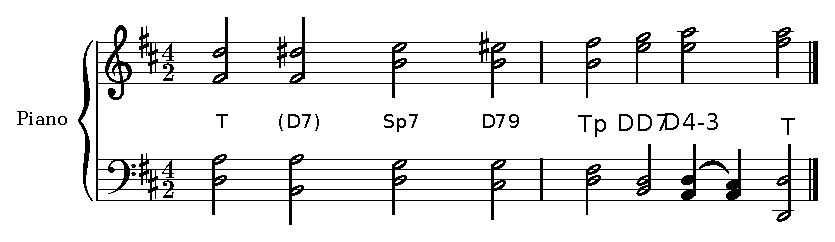
\includegraphics[width=0.8\textwidth]{frontends/nted/candenca2-ntd}
\end{center}

\acc{NtEd} erlaubt den Export im Bild\footnote{PS, PNG, PDF, SVG},
Ton\footnote{Midi}- und \acc{LilyPond}-Format. Der \acc{LilyPond}-Code ist --
sofern man auf textuelle Auszeichnung verzichtet -- klar strukturiert, also zur
Weiterverarbeitung geeignet. Unglücklicherweise scheitert die die
Verifikation\footnote{$\rightarrow$ S.\pageref{ExportVerifikation}} der von NtEd
exportierten \acc{LilyPond}-Datei. Um sie prozessierbar zu machen, sie enthält
mussten wir eine Klammer auskommentieren:

\begin{verbatim}
StaffAVoiceA = \relative c' {
   < fis d' >2  < fis dis' >  < b e >  < b f > | % 2
   < b fis' >  < e g >  < e a >  < fis a > 
  \bar "|."
}

StaffA = \new Staff \relative c' {\clef treble\key d \major \time 4/2
  <<
    \new Voice = "one" { \StaffAVoiceA } 
  >>
}

StaffBVoiceA = \relative c' {
   < d, a' >2  < b a' >  < d g >  < cis g' > | % 2
   < d fis >  < b d >  < a d >4 (   < a cis > )   < d, d' >2 
  \bar "|."
}

StaffB = \new Staff \relative c' {\clef bass\key d \major \time 4/2
  <<
    \new Voice = "one" { \StaffBVoiceA } 
  >>
}

\score {
  <<
    \new PianoStaff 
    <<
      \StaffA
%    >> DIESE KLAMMER IST ZUVIEL
      \StaffB
    >>
  >>
  \layout { }
}
\end{verbatim}

Aufs Ganze gesehen wird \acc{NtEd} allenfalls für den Musikwissenschaftler als
'erleichterndes' \acc{LilyPond}-Frontend in Frage kommt, der bereits mit
\acc{NtEd} arbeitet. Sich sein Handling neu anzueignen, ist wenig sinnvoll;
Aufwand, Ergebnis und Wiederverwendbarkeit stehen angesichts des
Entwicklungsstatus nicht im Einklang. Will man als Musikwissenschaftler
\acc{NtEd} dennoch nutzen, kann man darin die Basisversion seines Notentextes
editieren, diese als acc{LilyPond}-Version exportieren und das Ergebnis
anschließend 'manuell' mit einem Texteditor verbessern.

Wir geben dem Programm 2 von 5 Sternen, weil es historisch gesehen durchaus
Verdienste hat und weil es auch heute noch funktioniert.


% this is only inserted to eject fault messages in texlipse
%\bibliography{../bib/literature}
 

% mycsrf 'for beeing included' snippet template
%
% (c) Karsten Reincke, Frankfurt a.M. 2012, ff.
%
% This text is licensed under the Creative Commons Attribution 3.0 Germany
% License (http://creativecommons.org/licenses/by/3.0/de/): Feel free to share
% (to copy, distribute and transmit) or to remix (to adapt) it, if you respect
% how you must attribute the work in the manner specified by the author(s):
% \newline
% In an internet based reuse please link the reused parts to mycsrf.fodina.de
% and mention the original author Karsten Reincke in a suitable manner. In a
% paper-like reuse please insert a short hint to mycsrf.fodina.de and to the
% original author, Karsten Reincke, into your preface. For normal quotations
% please use the scientific standard to cite
%




\subsubsection{Ptolemaic ($\bigstar$)}

\label{Ptolemaic}\acc{Ptolemaic} wird auf seiner Homepage -- sternenreich -- als
ein Programm zur Visualisierung und Untersuchung tonaler Musik offeriert, die
bei der Analyse \enquote{of all types of Western music} helfen könne und dazu
etablierte analytische Techniken nutze, \enquote{[\ldots] including tonal
functional analysis (Harrison 1994) [\ldots]}.\footcite[vgl.][\nopage
wp]{Ptolemaic2016a} Das Java-Programm wird als Paket zum Download angeboten, das
darin enthaltene \acc{jar}-File kann mit einem simplen \texttt{java -jar
Ptolemaic.jar} gestartet werden.\footnote{\cite[vgl.][\nopage
wp]{Ptolemaic2016b}. Unglücklicherweise ist die Lizensierung unklar.} Es liest
\acc{MusicXML}-Dateien ein und exportiert \acc{seq}-Files.

Unsere Referenzkadenz II vermag \acc{Ptolemaic} in der \acc{MusicXML}-Version
erfolgreich zu laden, die \acc{Canorus} exportiert, nicht ohne allerdings das
angebliche Fehlen einer \enquote{tonicization} anzumahnen. Die
\acc{MusicXML}-Version der Refrenzkadenz II, die wir deshalb aus \acc{MuseScore}
heraus 'ersatzweise' exportiert haben, kann \acc{Ptolemaic} überhaupt nicht mehr
öffnen: es scheint dabei in eine Schleife zu geraten. Nach dem Einlesen der
Referenkadenz II bietet \acc{Ptolemaic} zwei Fenster an. Das eine enthält eine
Visualisierung der Töne in Form von Balken, das andere eine daraus abgeleitete
harmonische Analyse:

\begin{center}
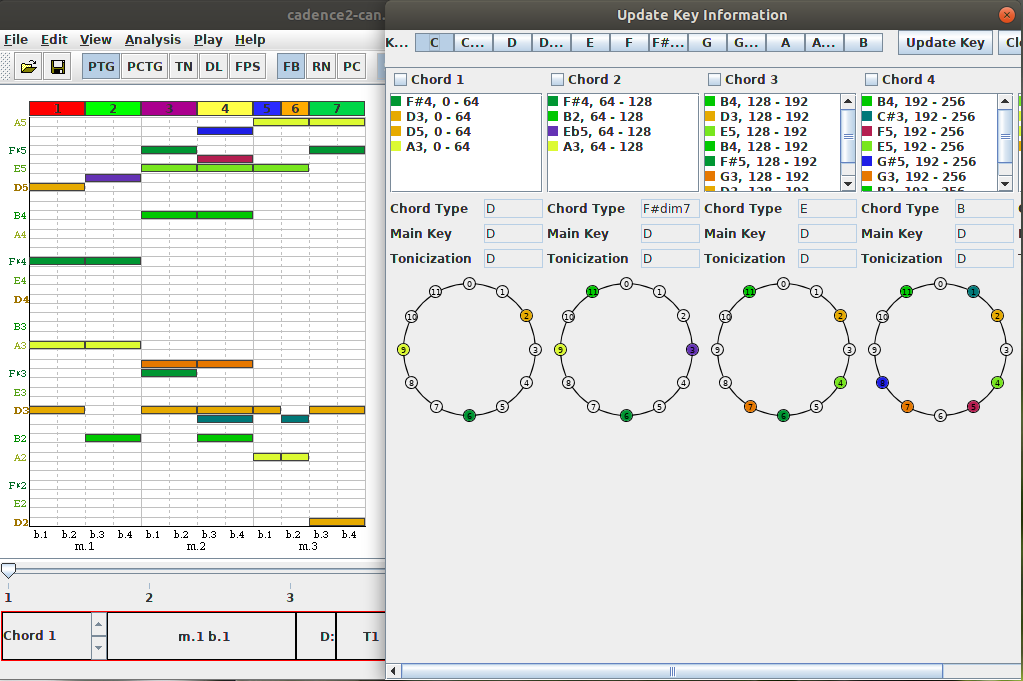
\includegraphics[width=0.9\textwidth]{frontends/ptolemaic/ptolemaic-2-win-300dpi.png}
\end{center}

Auch wenn \acc{Ptolemaic} über das Menue noch andere Analysen anbietet,
generiert es keine 'Noten', die man in einem \LaTeX-Text einbetten könnte, nicht
einmal als Bild. Außerdem erlaubt es vorderhand nicht, seine Analyseergebnisse
textuell zu exportieren. Von daher bietet \acc{Ptolemaic} hier wirklich keine
Unterstützung -- weder so, noch so.\footnote{Dass wir \acc{Ptolemaic} deshalb
nur einen Stern geben, ist in gewisser Hinsicht ungerecht: Man kann diesem
Programm kaum wirklich vorwerfen, unsere Ziele nur mangelhaft umgesetzt zu
haben. Es ist ja nur dadurch in unseren Blick geraten, dass es in der
MusicXML-Softwareseite gelistet wird (\cite[vgl.][\nopage
wp]{MusicXML2018b}). \acc{Ptolemaic} selbst ist gar nicht angetreten, den
Notendsatz zu unterstützen. Und da es das tut, was es wirklich tun will, wären 3
Sterne eigentlich angemessen. Wir belassen es trotzdem bei einem, weil es
gelegentlich abstürzt, Funktionen nicht ausführt und nicht bekennt, ob es nun
Open-Source-Software ist oder nicht.}

% this is only inserted to eject fault messages in texlipse
%\bibliography{../bib/literature}
 

% mycsrf 'for beeing included' snippet template
%
% (c) Karsten Reincke, Frankfurt a.M. 2012, ff.
%
% This text is licensed under the Creative Commons Attribution 3.0 Germany
% License (http://creativecommons.org/licenses/by/3.0/de/): Feel free to share
% (to copy, distribute and transmit) or to remix (to adapt) it, if you respect
% how you must attribute the work in the manner specified by the author(s):
% \newline
% In an internet based reuse please link the reused parts to mycsrf.fodina.de
% and mention the original author Karsten Reincke in a suitable manner. In a
% paper-like reuse please insert a short hint to mycsrf.fodina.de and to the
% original author, Karsten Reincke, into your preface. For normal quotations
% please use the scientific standard to cite

%% use all entries of the bibliography

\subsection{Rosegarden ($\bigstar\bigstar\bigstar$)}

\parpic(1cm,1cm)[r][t]{
\includegraphics[width=1cm]{logos/rosegarden-300dpi.png}}
\label{Rosegarden}\acc{Rosegarden} versteht sich als Kompositionsumgebung, die
um einen 'MIDI Sequencer' herum aufgebaut worden sei und dabei auch als
Notensatz- und digitales Audiosystem fungiere.\footcite[vgl.][\nopage
wp.]{Rosegarden2019a} Als \enquote{MIDI and audio sequencer} und \enquote{musical
notation editor} wolle es \enquote{das Tool der Wahl} für jene sein, die es
vorziehen, mittels Noten zu arbeiten:\footnote{Im Original: \enquote{to serve as
the sequencer of choice for users who prefer to work with music notation}
(\cite[vgl.][\nopage wp.]{Rosegarden2019c})}

\begin{quote}\enquote{\textit{Rosegarden allows you to record, arrange, and compose
music, in the shape of traditional score or MIDI data, or of audio files either
imported or recorded from a microphone, guitar or whatever audio source you care
to specify.}}\footcite[vgl.][\nopage wp.]{Rosegarden2019c} \end{quote}

Man könne mit \acc{Rosegarden} Musik schreiben, editieren oder komponieren,
diese synthetisieren, mit Effekten anreichern oder abmischen, um sie schließlich
auf CD zu brennen. Und nicht zuletzt biete \acc{Rosegarden} eben den
\enquote{[\ldots] well-rounded notation editing support for high quality printed
output via LilyPond}.\footcite[vgl.][\nopage wp.]{Rosegarden2019c}

Stellt man dem die These zur Seite, dass der \enquote{Kern eines Sequenzers
[\ldots] die Speicherung und Über\-mitt\-lung einer Partitur an einen
Tonerzeuger (sei)}, die \enquote{ [\ldots] in einem maschinenlesbaren Format
(vorliege)}, und dass diese Partitur \enquote{[\ldots] Tonhöhe, Tondauer und
ggf. weitere Aspekte der wiederzugebenden Noten einer oder mehrerer Stimmen in
ihrer zeitlichen Reihenfolge an ein Gerät (weitergäbe), das entsprechende Töne
(erzeuge)}\footcite[vgl.][\nopage wp.]{WpedSequencer2018a}, dann gewinnt man
damit eine recht genaue Vorstellung von dem, was \acc{Rosegarden} leisten will:
Es erlaubt den Import von \acc{MIDI}-Aufnahmen, bietet die Möglichkeit, diese zu
korrigieren, zu modifizieren, zu arrangieren und wieder
abzuspielen\footcite[vgl.][\nopage wp.]{Rosegarden2019c}. Ein Seiteneffekt des
Angebots ist, dass diese Modifikationen auch visuell über einen Noteneditor
erfolgen können.\footcite[vgl.][\nopage wp.]{Rosegarden2019d}

Als Open-Source-Software wird der Quelltext von \acc{Rosegarden} öffentlicht
gehostet und weiterentwickelt.\footnote{\cite[vgl.][\nopage
wp.]{Rosegarden2019e}. Die Projektseite gibt an, das Programm werde unter der
GPL-2.0 Lizenz distribuiert. Damit ist \acc{LilyPond} freie Software.} Die
Dokumentation wird als Wiki gepflegt\footcite[vgl.][\nopage wp.]{Rosegarden2019c}
und auch in thematischen Teilenbereichen bereitgestellt\footcite[vgl.][\nopage
wp.]{Rosegarden2019d}. Daneben gibt es noch spezielle
Tutorials\footcite[vgl.][\nopage wp.]{Rosegarden2019b}, die ausgehend von einem
bestimmten Aspekt in die Nutzung von \acc{Rosegarden}
einführen.\footcite[vgl.][\nopage wp.]{McIntyre2008a}

Vom Format her erlaubt es \acc{Rosegarden}, außer dem eigenen Dateityp auch
\acc{MIDI}- und \acc{MusicXML}-Dateien zu öffnen bzw. zu importieren. Beim Export
wird u.a. noch das \acc{LilyPond}-Format angeboten. Startet man einen
\acc{MIDI}-Server -- etwa \acc{timidity}\footnote{über eine Shell per
\texttt{timidity -iA}} --, bevor man \acc{Rosegarden} aufruft, können die
geladenen Noten außerdem erfolgreich abgespielt werden.

Unsere Referenzkadenz II vermag \acc{Rosegarden} problemlos als MusicXML-Datei
zu lesen, sofern diese keinen Text, also keine Harmonierungssymbole enhält.
Selektiert man beide Tracks und ruft über das Menue die Notenvisualierung
auf\footnote{\texttt{Select/Edit With/Open in Notation Editor}}, wird der
Notentext auf dem Bildschirm angezeigt:

\begin{center}
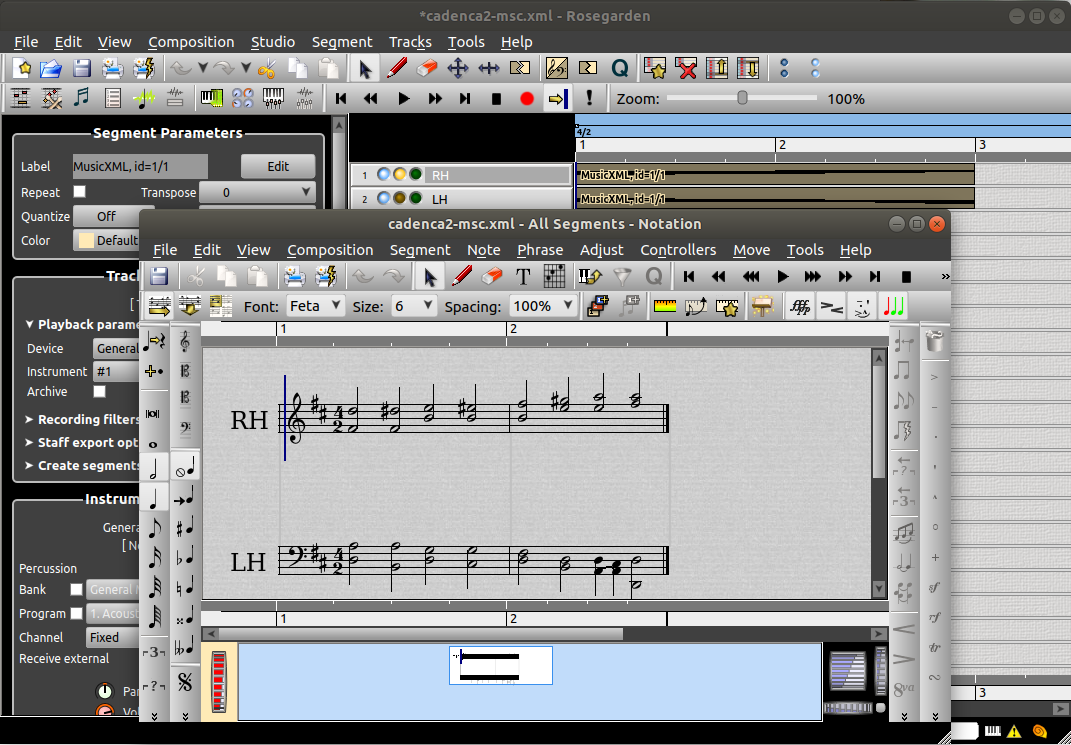
\includegraphics[width=0.9\textwidth]{frontends/rosegarden/rosegarden-cadenca2-300dpi.png}
\end{center}

Das Editieren des Notentextes ist gewöhnungsbedürftig, aber nicht unmöglich.
\acc{LilyPond}-Code kann nicht direkt eingegeben werden. Damit steht unsere
kleine Zusatzbibliothek für die Harmonieanalyse nicht zu Verfügung, allenfalls
die Umfunktionierung die normalen Liedtextfunktionalität. Wenn man unsere
Referenzkadenz als \acc{LilyPond}-Code exportiert, kann man das Ergebnis ohne
Abstriche z.B. in \acc{Frescobaldi} wieder einlesen.

Für die diejenigen, die ihre Musik eher über \acc{MIDI}-Kanäle eingeben wollen,
ist Rosegarden ein hervoragendes Frontend, ist doch seine optische Erscheinung
auf die spurenorientierte Bearbeitung von Musik auslegt. Die Funktion zum
Notensatz wirkt da etwas aufgesetzt. Für einen eher notenorientierten
Musikwissenschaftler wird Rosegarden nicht wirklich das Mittel der Wahl darstellen,
auch wenn es das, was es leisten will, ausgezeichnet tut. Insofern geben wir 
Rosengarden -- nur aus unserem Kontext heraus -- drei Sterne.


% this is only inserted to eject fault messages in texlipse
%\bibliography{../bib/literature}
 

\section{Vom Frontend in den \LaTeX-Text: die Toolkombination}

% mycsrf 'for beeing included' snippet template
%
% (c) Karsten Reincke, Frankfurt a.M. 2012, ff.
%
% This text is licensed under the Creative Commons Attribution 3.0 Germany
% License (http://creativecommons.org/licenses/by/3.0/de/): Feel free to share
% (to copy, distribute and transmit) or to remix (to adapt) it, if you respect
% how you must attribute the work in the manner specified by the author(s):
% \newline
% In an internet based reuse please link the reused parts to mycsrf.fodina.de
% and mention the original author Karsten Reincke in a suitable manner. In a
% paper-like reuse please insert a short hint to mycsrf.fodina.de and to the
% original author, Karsten Reincke, into your preface. For normal quotations
% please use the scientific standard to cite
%

\tikzstyle{nodv} = [font=\small, ellipse, draw, fill=gray!10, 
    text width=2cm, text centered, minimum height=2em]

\tikzstyle{nods} = [font=\footnotesize, rectangle, draw, fill=gray!20, 
    text width=1.2cm, text centered, rounded corners, minimum height=3em]

\tikzstyle{nodb} = [font=\footnotesize, rectangle, draw, fill=gray!20, 
    text width=2.2cm, text centered, rounded corners, minimum height=3em]

\tikzstyle{nodx} = [font=\footnotesize, rectangle, draw, fill=gray!20, 
    text width=2.4cm, text centered, rounded corners, minimum height=3em]
    
\tikzstyle{leaf} = [font=\tiny, rectangle, draw, fill=gray!30, 
    text width=1.2cm, text centered, minimum height=6em]

\tikzstyle{edge} = [draw, -latex']

\begin{tikzpicture}[]

%\node (l61) at ( 2.4, 9.2) {MIT};

%\node[nodb] (l51) at ( 0.0, 7.8) {\textit{recipient:} \\ \textbf{4yourself}};
% \node[nodb] (l52) at ( 4.8, 7.8) {\textit{recipient:} \\ \textbf{2others}};
% 
% \node[nodb] (l41) at ( 2.5, 6.2) {\textit{state:} \\ \textbf{unmodified}};
% \node[nodb] (l42) at ( 7.0, 6.2) {\textit{state:} \\ \textbf{modified}};
% 
% \node[nodb] (l31) at ( 5.0, 4.6) {\textit{type:} \\ \textbf{proapse}};
% \node[nodb] (l32) at ( 9.0, 4.6) {\textit{type:} \\ \textbf{snimoli}};
% 
% \node[nodx] (l21) at ( 7.5, 2.8) {\textit{context:} \\ \textbf{independent}};
% \node[nodx] (l22) at (10.5, 2.8) {\textit{context:} \\ \textbf{embedded}};
% 
% \node[leaf] (l11) at ( 0.0, 0.0) {\textbf{MIT-C1} \textit{using software only for yourself}};
% \node[leaf] (l12) at ( 2.5, 0.0) {\textbf{MIT-C2} \textit{distributing unmodified package}};
% \node[leaf] (l13) at ( 5.0, 0.0) {\textbf{MIT-C3} \textit{distributing modified program}};
% \node[leaf] (l14) at ( 7.5, 0.0) {\textbf{MIT-C4} \textit{distributing modified library as independent package}};



\node[leaf] (l14) at (1.0cm, 1.0cm) {Frescobaldi};

\node[leaf] (l15) at (0.0, 0.0) {MuseScore};


% \path [edge] (l61) -- (l51);
% \path [edge] (l61) -- (l52);
% \path [edge] (l51) -- (l11);
% \path [edge] (l52) -- (l41);
% \path [edge] (l52) -- (l42);
% \path [edge] (l41) -- (l12);
% \path [edge] (l42) -- (l31);
% \path [edge] (l42) -- (l32);
% \path [edge] (l31) -- (l13);
% \path [edge] (l32) -- (l21);
% \path [edge] (l32) -- (l22);
% \path [edge] (l21) -- (l14);
% \path [edge] (l22) -- (l15);

\end{tikzpicture}





% this is only inserted to eject fault messages in texlipse
%\bibliography{../bib/literature}
 

\section{Fazit}

%% mycsrf 'for beeing included' snippet template
%
% (c) Karsten Reincke, Frankfurt a.M. 2012, ff.
%
% This text is licensed under the Creative Commons Attribution 3.0 Germany
% License (http://creativecommons.org/licenses/by/3.0/de/): Feel free to share
% (to copy, distribute and transmit) or to remix (to adapt) it, if you respect
% how you must attribute the work in the manner specified by the author(s):
% \newline
% In an internet based reuse please link the reused parts to mycsrf.fodina.de
% and mention the original author Karsten Reincke in a suitable manner. In a
% paper-like reuse please insert a short hint to mycsrf.fodina.de and to the
% original author, Karsten Reincke, into your preface. For normal quotations
% please use the scientific standard to cite
%


%% use all entries of the bibliography
\section{Apendices}

\section{Sterne-Bewertung}

Wir werden die Tools nach einer einfachen
Systenmatik bewerten:
 
 %\begin{table}
\begin{center}
\begin{tabulary}{15cm}{R||C|C|C|C|C|}
\hline
\multirow{2}{*}{*} & 
  \multirow{2}{*}{Development} & 
  \multirow{2}{*}{Executability} & 
  \multirow{2}{*}{Musicscore} & 
  \multirow{2}{*}{Usability} & 
  Musicology  \\
 & &  &  &  & Support \\
\hline
\hline
$\bigstar$ 
  & outdated & inaccessible & ? & ? & ? \\
\hline 
$\bigstar\bigstar$ 
  & outdated & loadable & acceptable & unwieldy & indirect \\
\hline 
$\bigstar\bigstar\bigstar$ 
  & maintained & loadable & good & acceptable & indirect \\
\hline 
$\bigstar\bigstar\bigstar\bigstar$ 
  & maintained & loadable & nifty & smart & indirect \\
\hline 
$\bigstar\bigstar\bigstar\bigstar\bigstar$ 
  & maintained & loadable & fancy & impressive & direct \\
\hline 
\hline
\end{tabulary}
\end{center}
%\end{table}

% this is only inserted to eject fault messages in texlipse
%\bibliography{../bib/literature}

% insert the nomenclature here

% mycsrf Deutsch Nomenclation Tokens Include Module 
%
% (c) Karsten Reincke, Frankfurt a.M. 2012, ff.
%
% This file is licensed under the Creative Commons Attribution 3.0 Germany
% License (http://creativecommons.org/licenses/by/3.0/de/): 
% For details see teh file LICENSE in the top directory

% specific abbreviations
\abbr[utb]{UTB}{Uni-Taschenbuch}
\abbr[stw]{stw}{suhrkamp taschenbuch wissenschaft}% mycsrf  Deutsch Nomenclation Tokens Include Module 

% general abbreviations
\abbr[vgl]{vgl.}{vergleiche}
\abbr[aaO]{a.a.O.}{am angegebenen Ort}
\abbr[ds]{ds.}{kollektiv für ders., dies., \ldots}
\abbr[ebda]{ebda.}{ebenda}
% \abbr[id]{id.}{idem = latin for 'the same', be it a man, woman or a group\ldots}
% \abbr[ibid]{ibid.}{ibidem = latin for 'at the same place'}
\abbr[ifross]{ifross}{Institut für Rechtsfragen der Freien und Open Source
Software}
% \abbr[lc]{l.c.}{loco citato = latin for 'in the place cited'}
\abbr[wp]{wp.}{webpage = Webdokument ohne innere Seitennummerierung}
%% mycsrf English Nomenclation Tokens Include Module 
%
% (c) Karsten Reincke, Frankfurt a.M. 2012, ff.
%
% This file is licensed under the Creative Commons Attribution 3.0 Germany
% License (http://creativecommons.org/licenses/by/3.0/de/): 
% For details see teh file LICENSE in the top directory
%

\abbr[afda]{AfdA}{Anzeiger für deutsches Altertum}
%\abbr[zfda]{ZfdA}{Zeitschrift für deutsches Altertum und deutsche Literatur [ISSN: 00442518]}
%\abbr[zfaw]{}{Zeitschrift für Allgemeine Wissenschaftstheorie / Journal for General Philosophy of Science [ISSN: 0044-2216]}

\printnomenclature

% insert the bibliographical data here
\bibliography{bib/literature}

\end{document}
